% Licencia y derechos: consulte ../../LICENSE-CC-BY-4.0.
% Las figuras y demás materiales de terceros pueden tener derechos separados y deben identificarse.

\chapter{Respuesta de frecuencia de circuitos electrónicos} %p2lo

\section{Introducción} %p2
Al iniciar el análisis de un circuito electrónico, generalmente se calcula primero el punto de operación, es decir los niveles de tensión y corriente para corriente continua. Después se considera el comportamiento del circuito para pequeñas variaciones de señal, en donde se cortocircuitan los condensadores grandes, y los modelos de los dispositivos desprecian los efectos reactivos. En resumen, se determina el funcionamiento del circuito solamente para 2 valores de frecuencia: corriente continua yu un valor superior pero indeterminado. En este tema, pretendemos ampliar el análisis a un rango mayor de frecuencias. En primer ligar esto exige aplicar conocimientos de análisis frecuencial de circuitos pasivos a circuitos con elementos electrónicos, y además requerirá un modelo de frecuencia de los elementos electrónicos que contemple efectos reactivos, como por ejemplo, pequeñas capacitancias internas.

Empezamos nuestra discusión con un repaso de los conceptos más elementales del análisis de circuitos lineales.

\section{Fundamentos de la respuesta frecuencial} %p2
Una onda senoidal esta caracterizada por su frecuencia, su fase y su amplitud, como se indica en la figura \ref{fig:basic_sine-wave}.

\begin{figure}[h]
	\centering
	\includegraphics[width=0.9\linewidth]{_fig/basic_sine-wave.pdf}
	\caption{Caracterización de señal senoidal}
	\label{fig:basic_sine-wave}
\end{figure}

Si excitamos un sistema lineal, $H(s)$, con una señal senoidal, la salida será de la misma frecuencia, $\omega_0$, pero su amplitud y fase serán modificados por el sistema. En la figura \ref{fig:basic_ls-response} se plantean tres casos:

\begin{enumerate}
	\item se aplica la señal $a cos(\omega_0 t)$ y se obtiene a la salida $A_0 cos(\omega_0 t + \theta_0)$
	\item a otra frecuencia se obtiene otra respuesta de la amplitud y de la fase, se aplica la señal $a cos(\omega_1 t)$ y se obtiene a la salida $A_1 cos(\omega_1 t + \theta_1)$
	\item si se combinan las entradas, las salidas se combinan linealmente: se aplica la señal $a (cos(\omega_0 t + \omega_1 t)$ y se obtiene a la salida $A_0 cos(\omega_0 t + \theta_0) + A_1 cos(\omega_1 t + \theta_1)$
\end{enumerate}

\begin{figure}[h]
	\centering
	\includegraphics[width=0.9\linewidth]{_fig/basic_ls-response.pdf}
	\caption{Respuesta de sistemas lineales}
	\label{fig:basic_ls-response}
\end{figure}

Es decir, la respuesta del sistema a una señal de frecuencia radial $\omega$ es igual si ocurre en forma aislada o como parte de una señal complicada. Esto es muy conveniente que nos permite determinar la respuesta de un sistema a una señal complicada al conocer individualmente la respuesta a cada frecuencia que la compone.

\subsection{Sistemas naturales generadores de señal periódica} %p4
\begin{description}
	\item[Cuerdas de una guitarra:] Vibran, yu por lo tanto resuenan a una frecuencia particular. En general, la música es una combinación complicada de diferentes frecuencias.
	\item[Diapasón:] Resuena a una frecuencia natural, que es función del material, su tamaño y forma.
	\item[Pulso cardíaco:] Una señal con frecuencia de repetición de aproximadamente un ciclo por segundo, pero compuesto por varias frecuencias para darle una forma característica, que se muestra en la figura \ref{fig:sn_pulso-cardiaco}.
\end{description}

\begin{figure}[h]
	\centering
	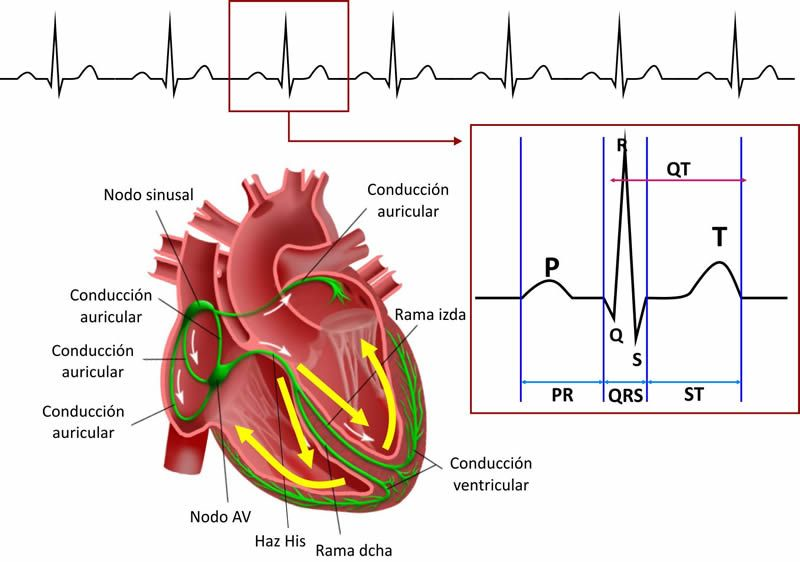
\includegraphics[width=0.9\linewidth]{_fig/sn_pulso-cardiaco.png}
	\caption{Distribución del impulso cardíaco y ondas e intervalos del electrocardiograma}
	\label{fig:sn_pulso-cardiaco}
\end{figure}

\subsection{Ejemplo de respuesta de sistema natural} %p4
En la figura \ref{fig:sn_audicion} se muestra la respuesta del sistema auditivo humano en la forma de la gráfica de sensibilidad de audición.

\begin{figure}[h]
	\centering
	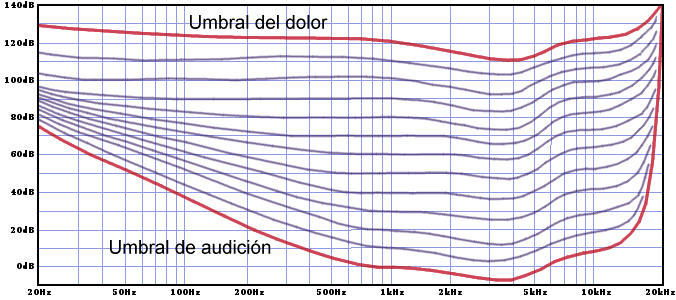
\includegraphics[width=0.9\linewidth]{_fig/sn_audicion.png}
	\caption{Umbral de dolor y umbral de audición}
	\label{fig:sn_audicion}
\end{figure}

Es decir, se requiere menos potencia de la fuente para escuchar un sonido de $3 kHz$ al cual somo más sensibles. Para escuchar un sonido de $100 Hz$ con la misma fuerza, la potencia real del sonido tiene que se mucho más grande. Las diferencias son tan grandes que se acude al uso de una escala logarítmica, con unidades en decibelios.

Si la respuesta para $1 KHz$ es $1$, la respuesta para $100 kHz$ es $0,01$. La respuesta relativa es $0.01/1$; en $dB$ es:

$20 log(0,01/1) = 20 log 10^{-2} = -40 dB$

\begin{figure}[h]
	\centering
	\includegraphics[width=0.6\linewidth]{_fig/respfreq_sch_hp.pdf}
	\caption{Circuito eléctrico}
	\label{fig:respfreq_sch_hp}
\end{figure}

\subsection{Respuesta de un sistema eléctrico} %p5

En la figura \ref{fig:respfreq_sch_hp} se muestra un circuito RC. A frecuencias bajas el condensador bloquea el paso de corriente, y se tiene $V_o = 0$. A frecuencias muy elevadas el condensador tiene una reactancia muy pequeña y $V_o = V_i$.

Para el circuito de la figura \ref{fig:respfreq_sch_hp}, se tiene:

$i = C \partial \frac{V_c}{\partial t} = C \partial \frac{V_i - V_o}{\partial t}$

$V_o = i R = C R \partial \frac{V_i - v_o}{\partial t}$

luego...

$C R \partial \frac{V_i}{\partial t} = V_o + C R \partial \frac{V_o}{dt}$

Podríamos resolver la ecuación diferencial al encontrar la respuesta natural en conjunto con la respuesta forzada de la señal de entrada para determinar $V_o$ dado $V_i$, por ejemplo si $V_i$ es una sinusoidal de frecuencia $\omega$. Analíticamente, un método más cómodo para establecer la relación entre $V_o$ y $V_i$ es por medio del análisis en el dominio $s$. La impedancia viene dada por la relación entre las variables de voltaje y corriente para un elemento:

\begin{tabular}{ccccc}
	$i = C \frac{\partial v}{\partial t}$ & $--->$ & $I = C S V$ & y & $Z = \frac{V}{I} = \frac{1}{C S}$ \\
	$v = L \frac{\partial i}{\partial t}$ & $--->$ & $V = L S I$ & y & $Z = \frac{V}{I} = L S$ \\
	$v = R i$ & $--->$ & $V = R I$ & y & $Z = \frac{V}{I} = R$ \\
\end{tabular}

La excitación del sistema es de la forma $e$.

\begin{figure}[h]
	\centering
	\includegraphics[width=0.6\linewidth]{_fig/respfreq_sch_hp_s.pdf}
	\caption{Circuito eléctrico, dominio S}
	\label{fig:respfreq_sch_hp_s}
\end{figure}

El circuito de la figura \ref{fig:respfreq_sch_hp} queda como se muestra en la figura \ref{fig:respfreq_sch_hp_s}, y nos da:

\begin{equation}\label{eqn:rse_1}
	\frac{V_i}{R + \frac{1}{CS}}=\frac{V_o}{R}
\end{equation}

\begin{equation}\label{eqn:rse_2}
	\frac{V_o}{V_i(S)} = \frac{R}{R + \frac{1}{C S}}
\end{equation}

\begin{equation}\label{eqn:rse_3}
	H(S) = \frac{V_o}{V_i(S)} = \frac{R}{R + \frac{1}{C S}}
\end{equation}

donde $H(S)$ es la función de transferencia del sistema; $H(S)$ nos determina los cambios de amplitud y de fase introducidos por el sistema donde la frecuencia de $V_o(t)$ es igual a la de $V_i(t)$.

"$S$" es un número complejo formado por una parte real y una parte imaginaria: $S = \Re + \Im\omega$

Un polo de $H(S)$, $S_p$, hace la función infinita, $H(S_p) = \infty$; mientras que un cero de $H(S)$, $S_z$, hace que la función cero, $H(S_z) = 0$. Para el caso anterior, el polo del sistema está en $S_p = \frac{-1}{R C}$, mientras que el cero es $S = 0$.

Se puede hallar la respuesta en frecuencia reemplazando $S$ por $\Im\omega$, es decir $e^{S t} = e^{\Im \omega t} = cos(\omega t) + \Im sin(\omega t)$, y variando $\omega$.

Entonces,

\begin{equation}\label{eqn:rse_4}
	\frac{V_o}{V_i}(\omega) = \frac{R}{R - \frac{\Im}{C \omega}}
\end{equation}

Un número complejo puede ser representado alternativamente por un módulo y una fase.

\begin{equation}\label{eqn:rse_5}
	H(\Im \omega) = |H(\Im \omega)| \angle H(\Im \omega)
\end{equation}

donde...

\begin{equation}\label{eqn:rse_6}
	|H(\Im \omega)| = \sqrt{\Re^2(H(\Im \omega)) + \Im^2(H(\Im \omega))}
\end{equation}

\begin{equation}\label{eqn:rse_7}
	\angle H(\Im \omega) = \tan^{-1}\frac{\Im(H(j\omega))}{\Re(H(j\omega))}
\end{equation}

Alternativamente, se puede trabajar el denominador por separado. Por ejemplo si tenemos: $\frac{1}{a+bj}$

entonces $|\frac{1}{(a+bj)}| = \frac{1}{\sqrt{a^2+b^2}}$

y $\angle (\frac{1}{(a+bj)}) = \tan^{-1} \frac{b}{a}$

De la ecuación \eqref{eqn:rse_4}:

$|\frac{V_O}{V_I} (\omega)| = \frac{R}{\sqrt{R^2+{\frac{1}{C\omega}}^2}}$

y

$\angle \frac{V_0}{V_I} (\omega) = \tan^{-1} (\frac{1}{\omega CR})$

éstas ecuaciones se grafican en la figura \ref{fig:respfreq_hp}, cambio de variable de $\omega = 2 \pi f$ para trabajar en términos de frecuencia, considere que para las figuras siguientes se ha definido $Vi=1V$, $R=10k\Omega$ y $C=1nF$:

\begin{figure}[h]
	\centering
	\subfloat[Amplitud]
	{
		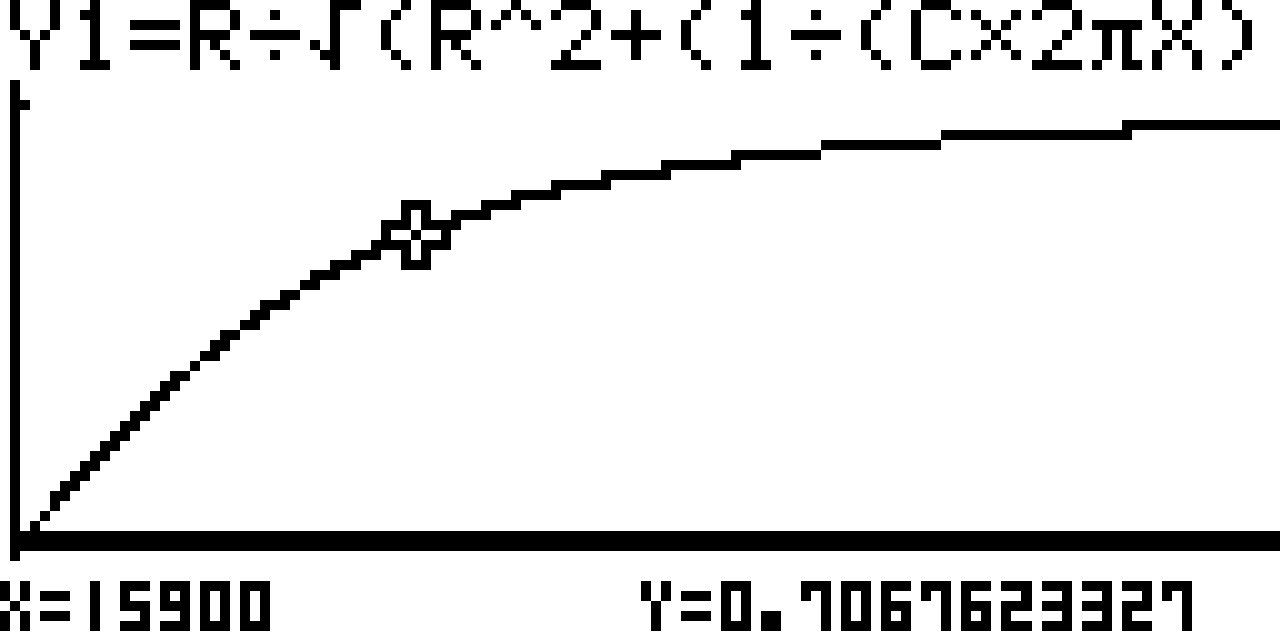
\includegraphics[width=0.4\linewidth]{_fig/respfreq_hp_abs.png}
		\label{fig:respfreq_hp_abs}
	}
	\subfloat[Angulo]
	{
		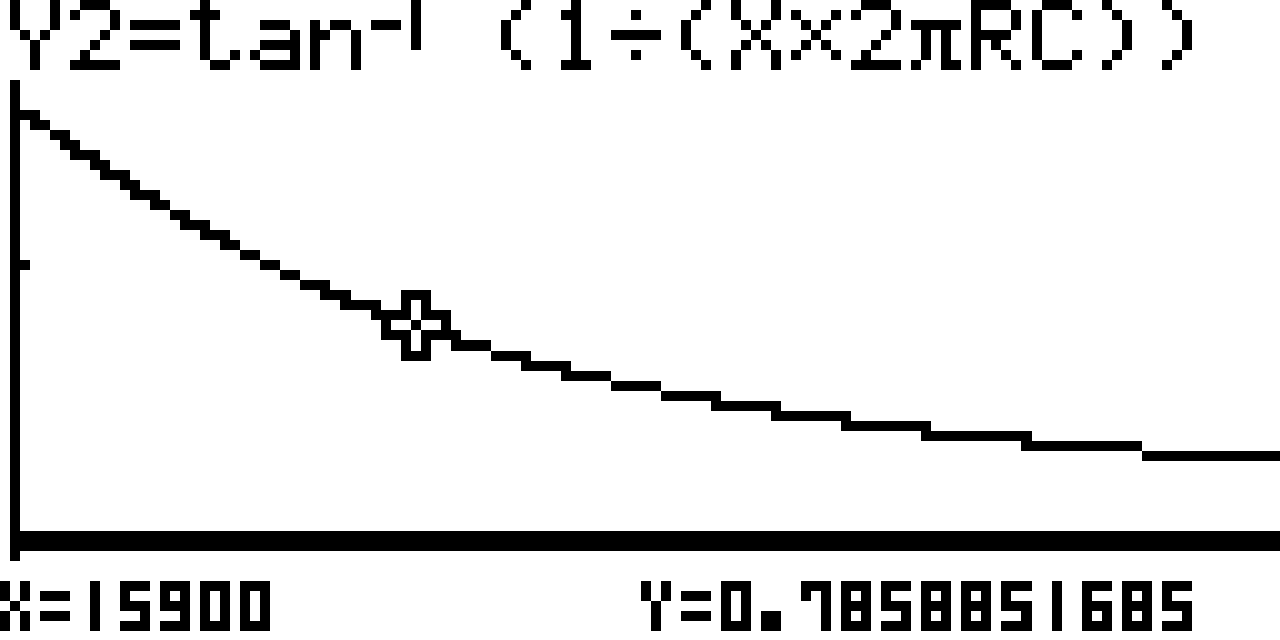
\includegraphics[width=0.4\linewidth]{_fig/respfreq_hp_ang.png}
		\label{fig:respfreq_hp_ang}
	}
	\caption{Respuesta en frecuencia, paso alto}
	\label{fig:respfreq_hp}
\end{figure}

Estas gráficas muestran la relación entre $V_O$ y $V_I$ a cualquier frecuencia. Por ejemplo, a la frecuencia $\omega=\frac{1}{2 \pi RC}$, $V_O$ tiene la $\frac{1}{\sqrt{2}}$ de amplitud de $V_I$(ver figura \ref{fig:respfreq_hp_abs}) y está desfasado $45^{\circ}$ o $\pi/4$ (ver figura \ref{fig:respfreq_hp_ang}).

\begin{figure}[h]
	\centering
	\subfloat[Gráfica $V_I$ y $V_O$]
	{
		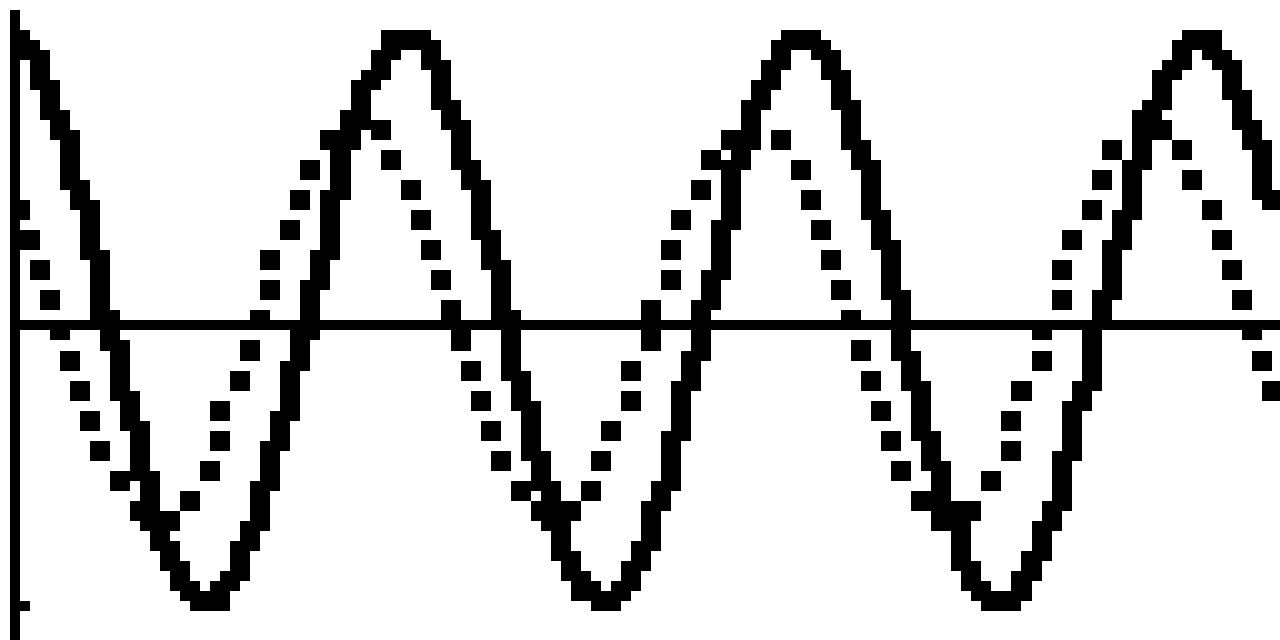
\includegraphics[width=0.4\linewidth]{_fig/respfreq_hp_vivo_plot.png}
		\label{fig:respfreq_hp_vivo_plot}
	}
	\subfloat[Ecuaciones]
	{
		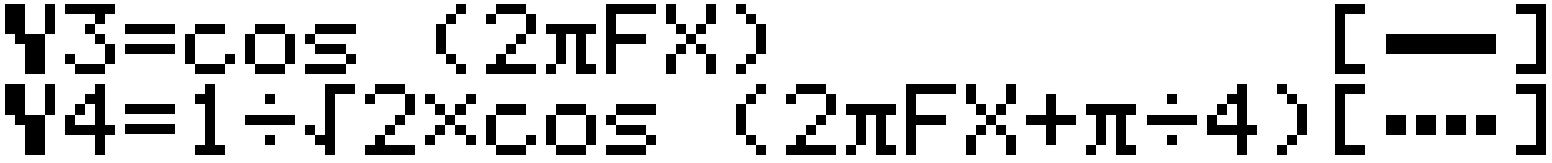
\includegraphics[width=0.4\linewidth]{_fig/respfreq_hp_vivo_eq.png}
		\label{fig:respfreq_hp_vivo_eq}
	}
	\caption{Relación entre $V_O$ y $V_I$ de la figura \ref{fig:respfreq_sch_hp} para $\omega=\frac{1}{2 \pi RC}$}
	\label{fig:respfreq_hp_vivo}
\end{figure}

La figura \ref{fig:respfreq_hp} representa un filtro paso alto: atenúa la señal de baja frecuencia, deja pasar la señal de alta frecuencia. En la figuras \ref{fig:respfreq_sch_lp} y \ref{fig:respfreq_lp} se muestra un filtro paso bajo.

\begin{figure}[h]
	\centering
	\includegraphics[width=0.6\linewidth]{_fig/respfreq_sch_hp.pdf}
	\caption{Circuito eléctrico, paso bajo}
	\label{fig:respfreq_sch_lp}
\end{figure}			

\begin{figure}[h]
	\centering
	\subfloat[Amplitud]
	{
		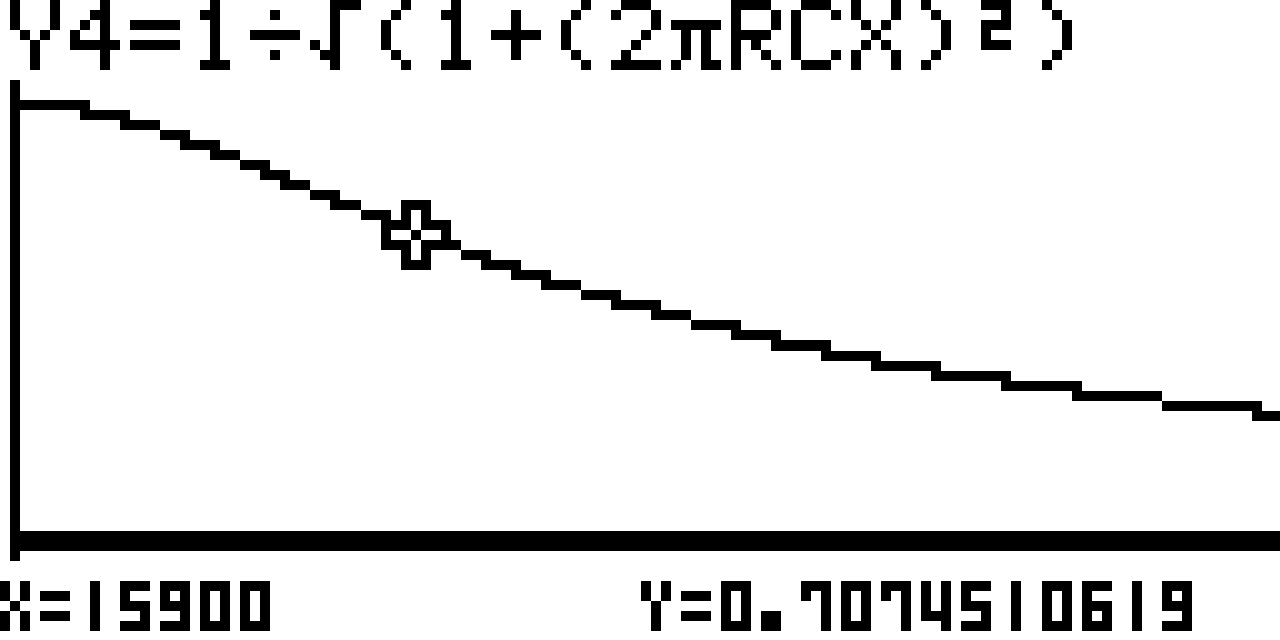
\includegraphics[width=0.4\linewidth]{_fig/respfreq_lp_abs.png}
		\label{fig:respfreq_lp_abs}
	}
	\subfloat[Angulo]
	{
		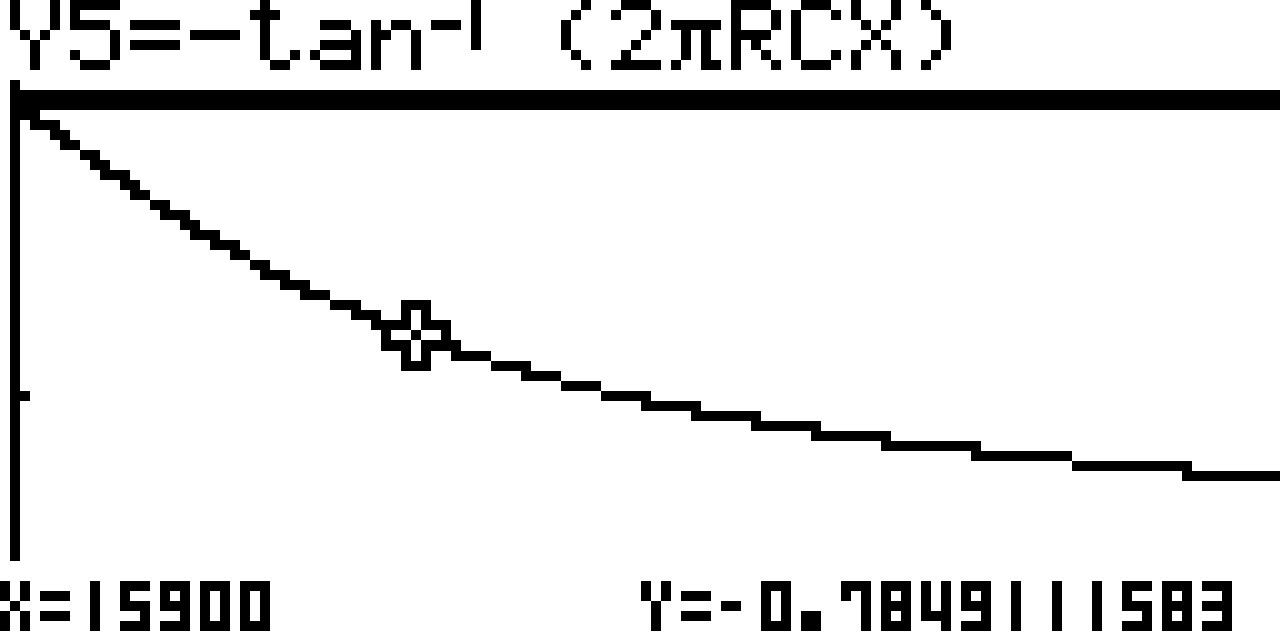
\includegraphics[width=0.4\linewidth]{_fig/respfreq_lp_ang.png}
		\label{fig:respfreq_lp_ang}
	}
	\caption{Respuesta en frecuencia, paso bajo}
	\label{fig:respfreq_lp}
\end{figure}

Bien se pueden resumir las respuestas de los filtros pasa alta y pasa baja de primer orden como se observan en las figuras \ref{fig:respfreq_summary_hp} y \ref{fig:respfreq_summary_lp}.

\begin{figure}[h]
	\centering
	\subfloat[Filtro paso alto]
	{
		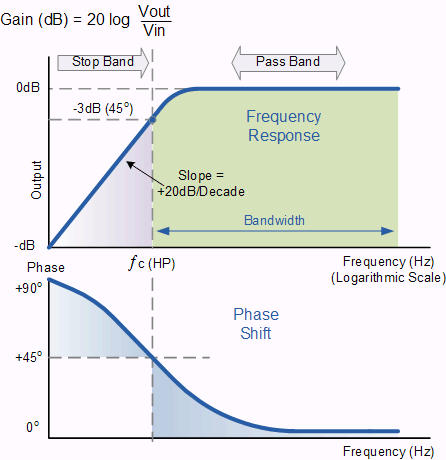
\includegraphics[width=0.4\linewidth]{_fig/respfreq_summary_hp.png}
		\label{fig:respfreq_summary_hp}
	}
	\subfloat[Filtro paso bajo]
	{
		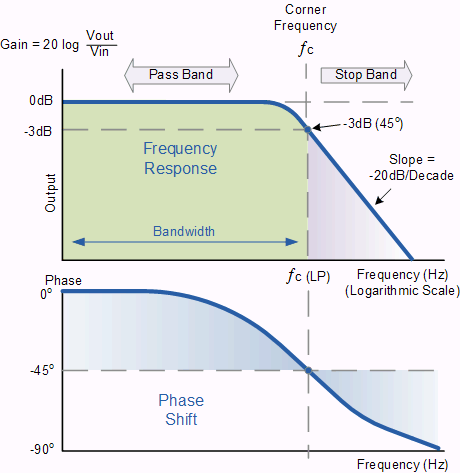
\includegraphics[width=0.4\linewidth]{_fig/respfreq_summary_lp.png}
		\label{fig:respfreq_summary_lp}
	}
	\caption{Respuesta en frecuencia, filtros de primer orden}
	\label{fig:respfreq_summary_hplp}
\end{figure}

\section{El diagrama de Bode} %p9

Los diagramas de Bode fueron ideados originalmente por el Dr. Henrik Wayne Bode mientras trabajaba para los Laboratorios Bell en la década de 1930. Se utilizan sobre todo para analizar la estabilidad de los sistemas de control, por ejemplo, al diseñar y analizar bucles de retroalimentación de la fuente de alimentación. La ventaja de utilizar el diagrama de Bode es que proporciona una forma sencilla y común de describir la respuesta de frecuencia de un sistema lineal invariante en el tiempo. Bode propuso graficar la respuesta de frecuencia en una escala logarítmica ya que de esta gráfica se podría distinguir información no fácilmente apreciable en la escala lineal.

Su motivación puede apreciarse de las gráficas de las funciones $H_1(S)$ y $H_2(S)$ en la figura \ref{fig:respfreq_bode} donde:

$H_1(S) = \frac{10}{1+\frac{S}{10}}$ y $H_2(S) = \frac{10}{(1+\frac{S}{15.625})^2}$

Las dos gráficas lucen idénticas; en particular no dejan distinguir dos diferencias importantes entre las funciones de transferencia:

\begin{enumerate}
	\item un sistema es de primer orden mientras que el otro es de segundo orden y...
	\item el valor de los polos en los dos sistemas difieren en un 50\%
\end{enumerate}

\begin{figure}[h]
	\centering
	\subfloat[$H_1(S)$]
	{
		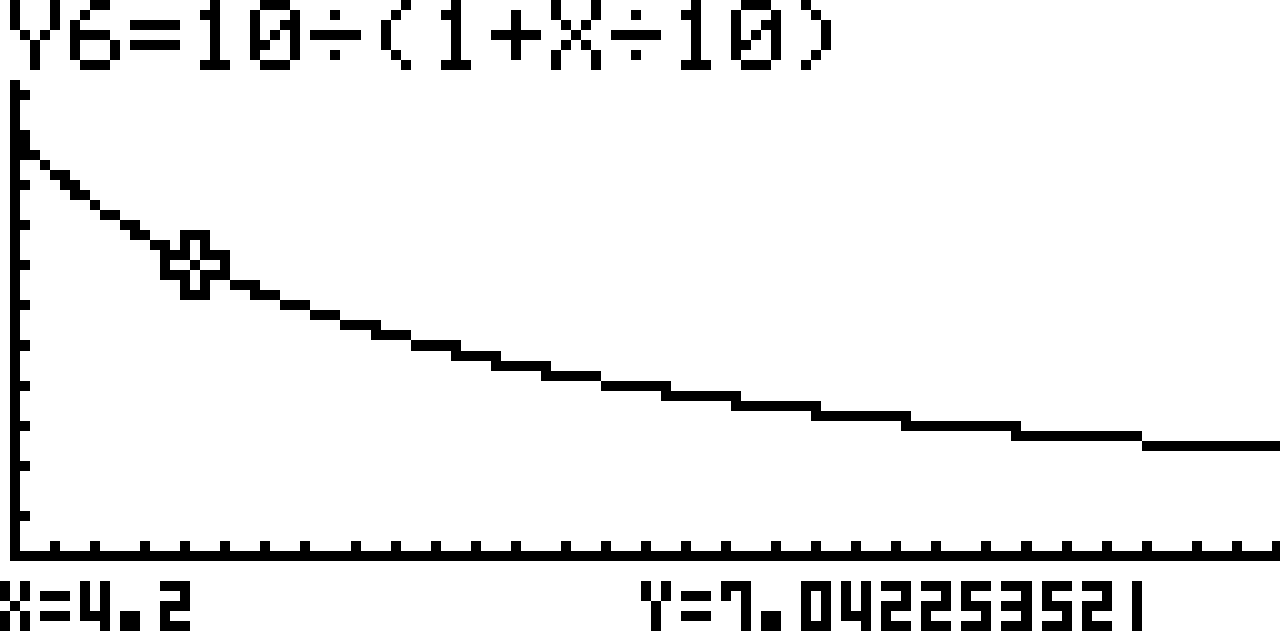
\includegraphics[width=0.4\linewidth]{_fig/respfreq_bode_h1.png}
		\label{fig:respfreq_bode_h1}
	}
	\subfloat[$H_2(S)$]
	{
		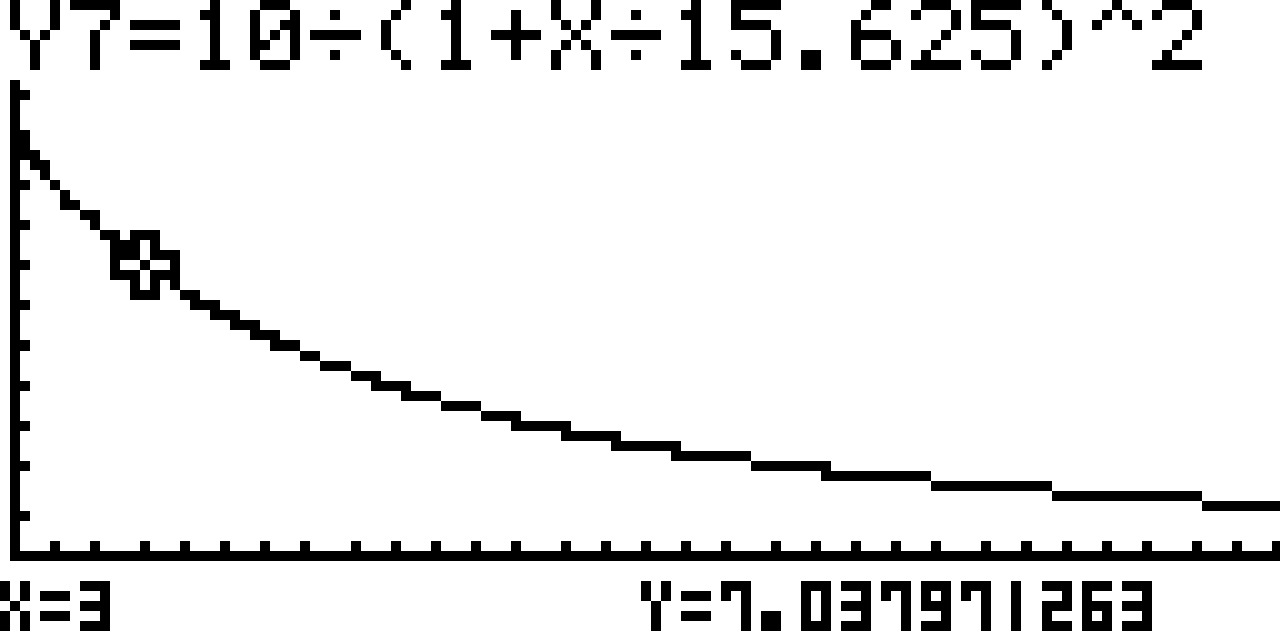
\includegraphics[width=0.4\linewidth]{_fig/respfreq_bode_h2.png}
		\label{fig:respfreq_bode_h2}
	}
	\caption{Respuestas $H_1(S)$ y $H_2(S)$}
	\label{fig:respfreq_bode}
\end{figure}

El diagrama de Bode es sencillamente la respuesta de frecuencia con la frecuencia en escala logarítmica, la magnitud en escala logarítmica, y la fase en escala lineal. Una aproximación a la curva se puede trazar a mano alzada sin necesidad de cálculos, sino en base a rectas y cambios de pendiente a las frecuencias de los polos y los ceros de la función de transferencia.

Dado una función generalizada de la forma:

\begin{equation}\label{eqn:rse_8}
	H(S) = \frac{a_mS^m + a_{m-1}S^{m-1} + ... + a_1S + q_0}{b_nS^n + b_{n-1}S^{n-1} + ... + n_1S + b_0}
\end{equation}

podemos expresarla para distinguir los ceros, los polos y una constantes:

\begin{equation}\label{eqn:rse_9}
	H(S) = a \frac{(S-Z_1)(S-Z_2) ... (S-Z_m)}{(S-p_1)(S-p_2) ... (S-p_n)}
\end{equation}

el módulo de $H(S)$ viene dado por:

\begin{equation}\label{eqn:rse_10}
	|H(S)| = a \frac{|S-Z_1||S-Z_2| ... |S-Z_m|}{|S-p_1||S-p_2| ... |S-p_n|}
\end{equation}

si ahora tomamos el logaritmo de ésta función y lo multiplicamos por $20$ se convierte en la forma apropiada para el Diagrama de Bode del módulo:

\begin{equation}\begin{split}\label{eqn:rse_11}
		20log|H(S)| = 20log|a| + 20log|S-Z_1| + 20log|S-Z_2| ... + 20log|S-Z_m| \\
		- 20log|S-P_1| - 20log|S-P_2| ... - 20log|S-P_n|
\end{split}\end{equation}

se hace notar como el producto de funciones se ha convertido en la suma de funciones para dar el total.

La fase de $H(S)$ se encuentra en la siguiente expresión:

\begin{equation}\begin{split}\label{eqn:rse_12}
		\angle|H(S)| = \angle a + \angle(S-Z_1) + \angle(S-Z_2) ... + \angle(S-Z_m) \\
		- \angle(S-P_1) - \angle(S-P_2) ... - \angle(S-P_n)
\end{split}\end{equation}

nuevamente la contribución de cada raíz y la constante se suma para obtener la total.

En la figura \ref{fig:respfreq_db_cero} se traza el Diagrama de Bode del módulo y la fase que contribuye un cero. Para el cero expresado de la forma $(1+\frac{S}{\omega})$, el módulo arranca a un nivel de $0 dB$ a frecuencias bajas, sube a $3 dB$ a la frecuencia del cero y eventualmente aumenta en forma proporcional a $\omega$, que en la escala logarítmica-logarítmica del Bode se representa con una pendiente de $20 dB$ por década (factor de diez) de frecuencia. La fase del cero arranca en $0^{\circ}$ a frecuencias bajas, sube a $5,17^{\circ}$ a una frecuencia 10 veces por debajo del cero, para por $45^{\circ}$ a la frecuencia del cero, llega a $84.83^{\circ}$ a una frecuencia 10 veces mayor que el cero hasta eventualmente llegar a un valor final de $+90^{\circ}$. Adicionalmente se dibuja asíntotas a las curvas reales. Hay varias formas de aproximar ésta curva real con rectas. La que se muestra aproxima la función $0^{\circ}$ hasta que la frecuencia $\frac{\omega_Z}{10}$, de allí subo con una recta de $\frac{45^{\circ}}{decada}$ en la escala lineal-logarítmica, para por $45^{\circ}$ a la frecuencia $\omega_Z$ hasta llegar a un valor final de $90^{\circ}$ a $10 \omega_Z$.

\begin{figure}[h]
	\centering
	\subfloat[Módulo]
	{
		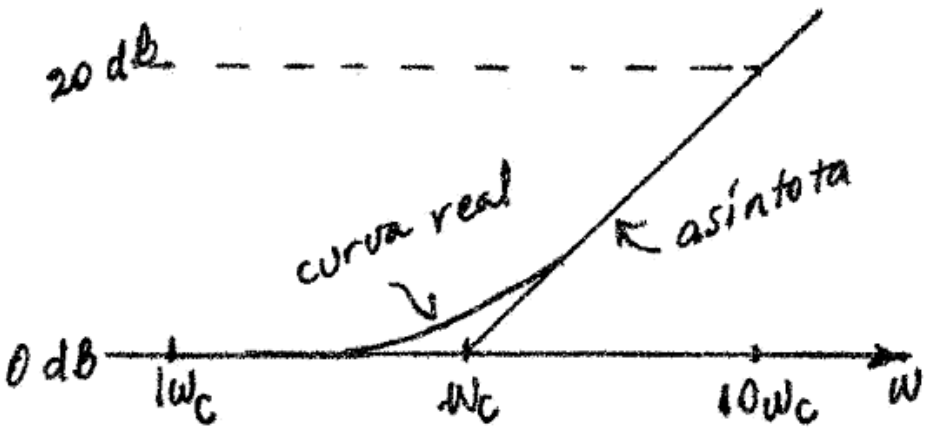
\includegraphics[width=0.4\linewidth]{_fig/respfreq_db_cero_modulo.png}
		\label{fig:respfreq_db_cero_modulo}
	}
	\subfloat[Fase]
	{
		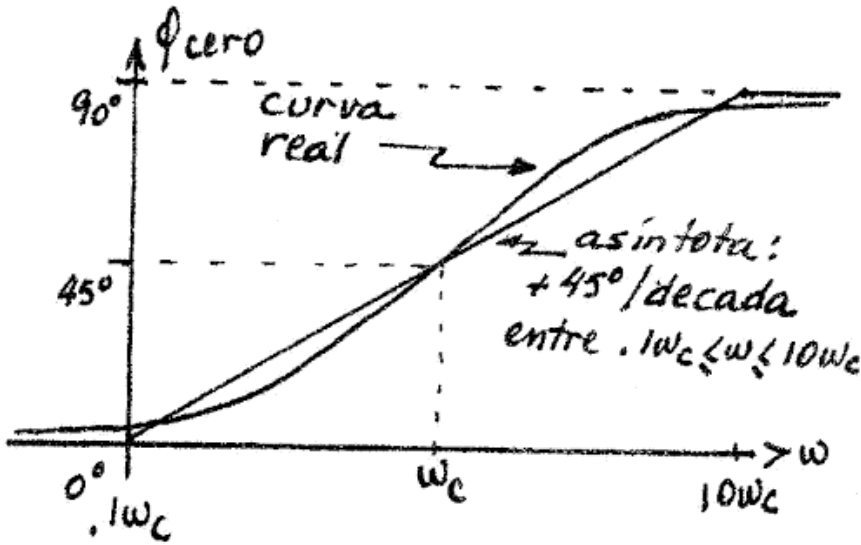
\includegraphics[width=0.4\linewidth]{_fig/respfreq_db_cero_fase.png}
		\label{fig:respfreq_db_cero_fase}
	}
	\caption{Diagrama de Bode de un Cero}
	\label{fig:respfreq_db_cero}
\end{figure}

En la figura \ref{fig:respfreq_db_polo} se traza el Diagrama de Bode del módulo y la fase que contribuye un polo. Se hace notar idénticas a las curvas del cero pero en sentido negativo. Para el polo expresado de la forma $1+\frac{S}{\omega}$, el módulo arranca a un nivel de $0 dB$ a frecuencias bajas, baja a $3 dB$ a la frecuencia del polo y eventualmente disminuye en forma proporcional a $\omega$, que en la escala logarítmica-logarítmica del Bode se representa con una pendiente de $-20 dB$ por década (factor de diez) de frecuencia. La fase del polo arranca en $0^{\circ}$ a frecuencias bajas. Baja a $-5,17^{\circ}$ a una frecuencia 10 veces por debajo del polo, pasa por $-45^{\circ}$ a la frecuencia del polo, llega a $84,83^{\circ}$ a una frecuencia 10 veces mayor que el polo hasta eventualmente llegar a un valor final de $-90^{\circ}$. Nuevamente se dibuja asíntotas a las curvas reales. La aproximación a esta curva real con rectas consta de un valor de $0$ hasta la frecuencia $\omega_P/10$, de allí baja con una recta de $\frac{-45^{\circ}}{decada}$ en la escala lineal-logarítmica, pasa por $-45^{\circ}$ a la frecuencia $\omega_P$ hasta llegar a un valor final de $-90^{\circ}$ a $10 \omega_P$.

\begin{figure}[h]
	\centering
	\subfloat[Módulo]
	{
		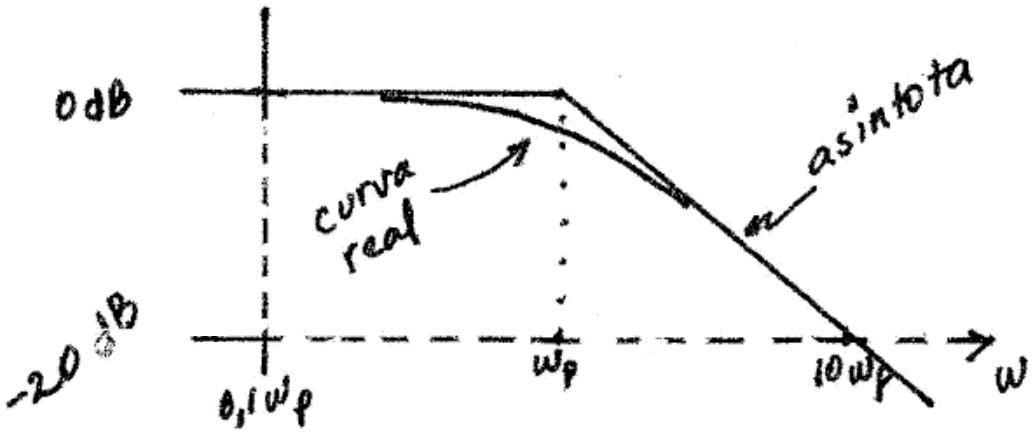
\includegraphics[width=0.4\linewidth]{_fig/respfreq_db_polo_modulo.png}
		\label{fig:respfreq_db_polo_modulo}
	}
	\subfloat[Fase]
	{
		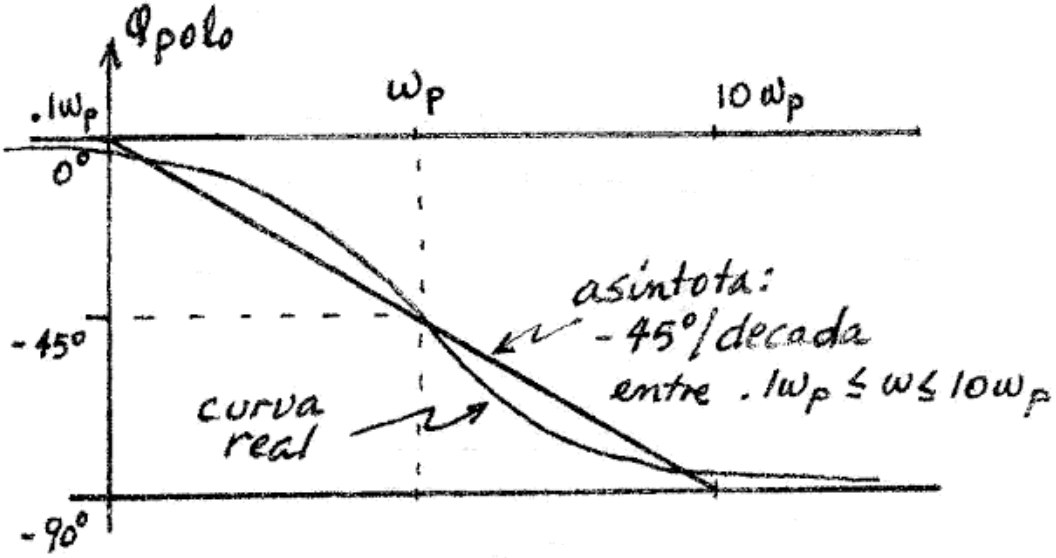
\includegraphics[width=0.4\linewidth]{_fig/respfreq_db_polo_fase.png}
		\label{fig:respfreq_db_polo_fase}
	}
	\caption{Diagrama de Bode de un Polo}
	\label{fig:respfreq_db_polo}
\end{figure}

Finalmente la constante contribuirá con un nivel de $20 log k$ al módulo, es decir, será constante, y su contribución a la fase será $0^{\circ}$ en caso de tratarse de un valor real y positivo, ó de $-180^{\circ}$ en caso de una constante real y negativa.

Por ejemplo, en la figura \ref{fig:respfreq_bode_h12_resp} se trazan los Diagramas de Bode de las funciones de transferencia con las cuales iniciamos esta sección:

$H_1(S) = \frac{10}{1+\frac{S}{10}}$ y $H_2(S) = \frac{10}{(1+\frac{S}{15.625})^2}$

Se comparan con la figura \ref{fig:respfreq_bode} y se puede apreciar mayor cantidad de información del sistema que puede obtenerse con la gráficas. Además las rectas que aproximan la curva real se trazan directamente sin necesidad de cálculos. El Diagrama de Bode es la forma preferida para el trazo de la respuesta en frecuencia de sistemas. Es particularmente útil para reflejar la atenuación exacta en la banda de atenuación.

\begin{figure}[h]
	\centering
	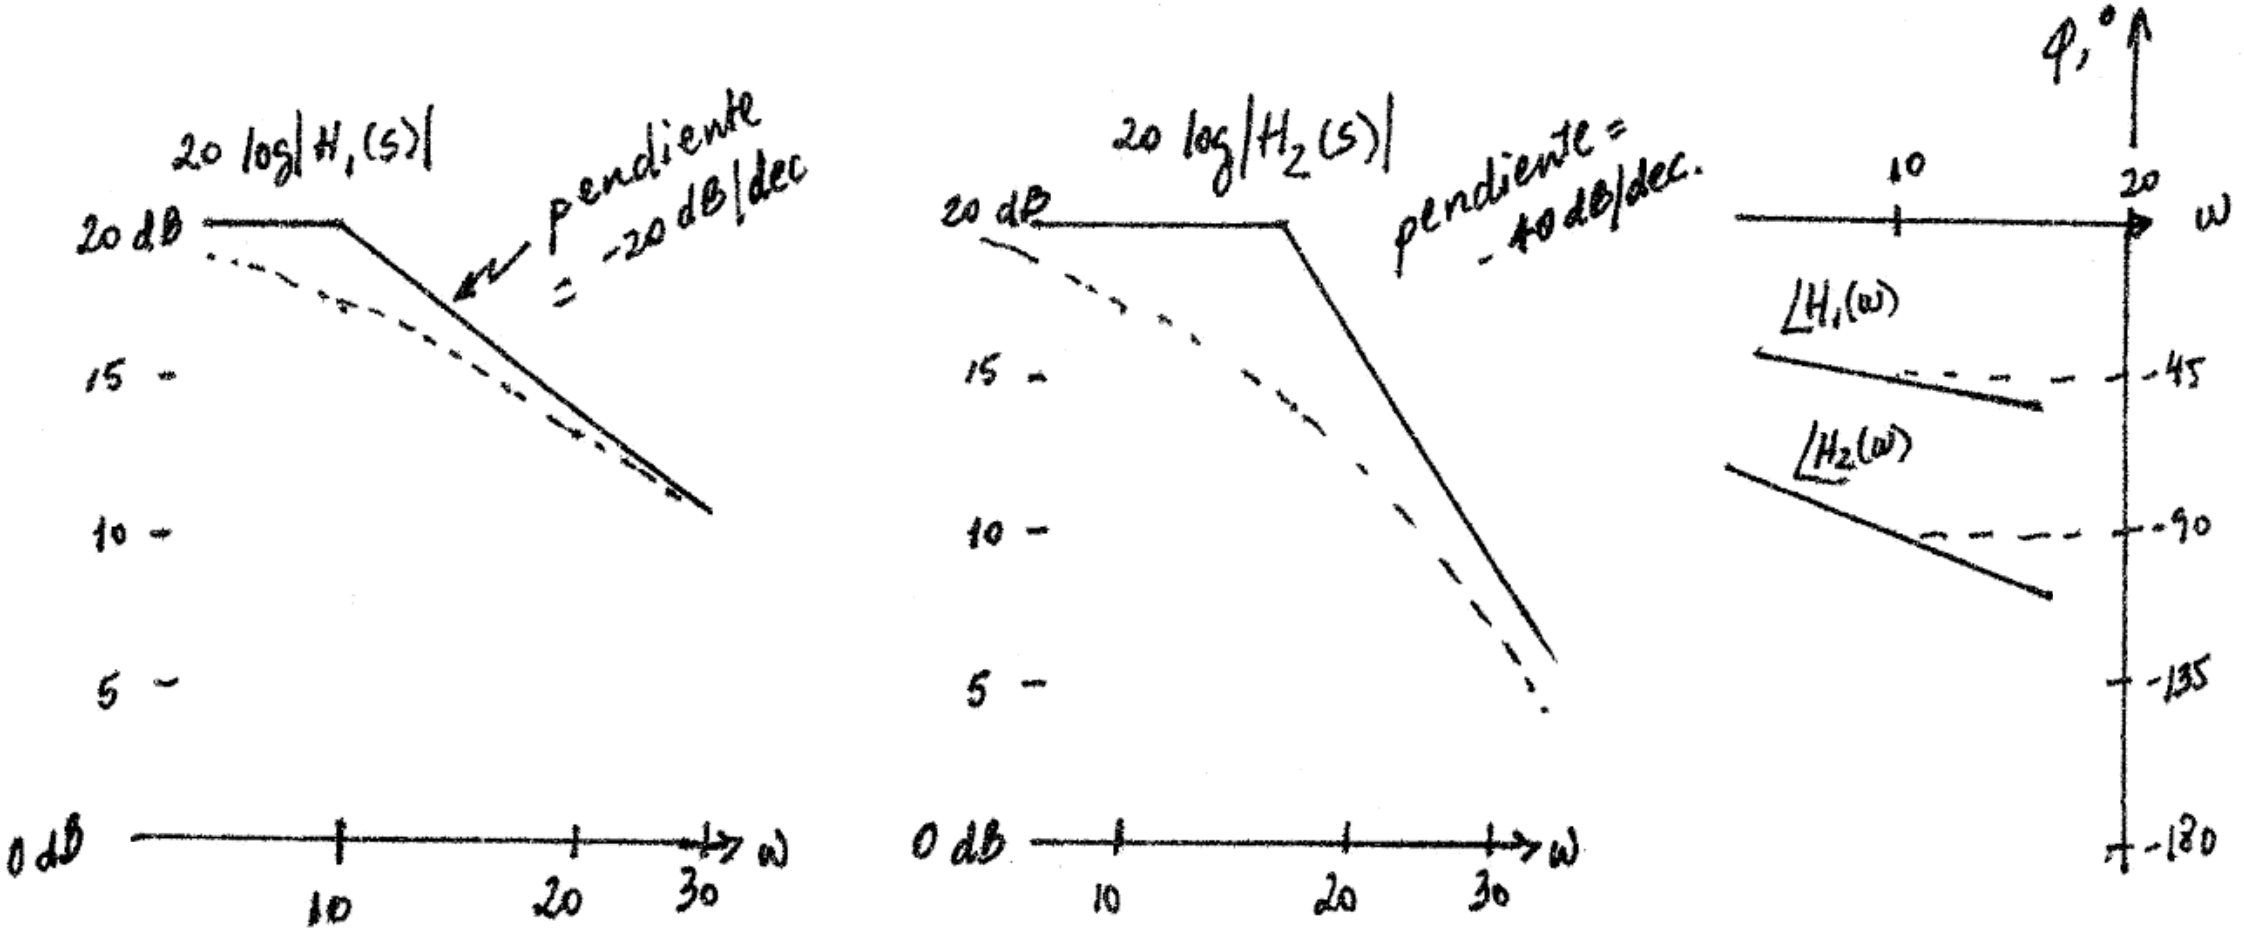
\includegraphics[width=0.9\linewidth]{_fig/respfreq_bode_h12_resp.png}
	\caption{Respuestas en Diagrama de Bode de $H_1(S)$ y $H_2(S)$}
	\label{fig:respfreq_bode_h12_resp}
\end{figure}

\section{Respuesta de los amplificadores} %p13

Existe una clase general de circuitos conocidos como amplificadores de banda ancha que se caracterizan por tener una ganancia constante en un rango relativamente ancho de frecuencias. Dentro de esta clase existen dos tipos: el amplificador de $DC$ y el amplificador acoplado capacitivamente.

En el amplificador DC, la señal es acoplada directamente entre etapas; la respuesta de frecuencia es como la que aparece en la Figura \ref{fig:respfreq_amp-dc}. 
El amplificador tiene una ganancia constante para un rango relativamente amplio de frecuencias, a partir de DC.

\begin{figure}[h]
	\centering
	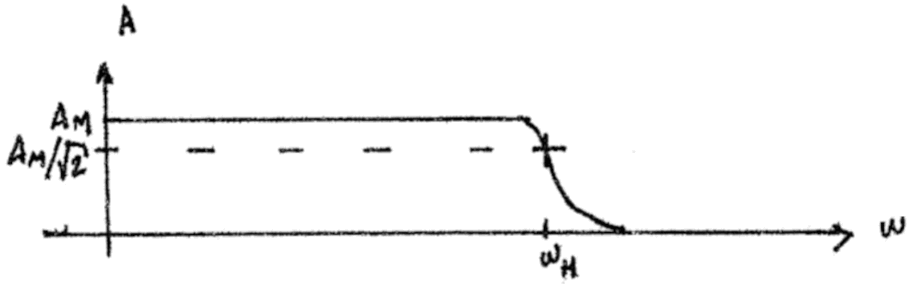
\includegraphics[width=0.9\linewidth]{_fig/respfreq_amp-dc.png}
	\caption{Respuesta de frecuencia del amplificador DC}
	\label{fig:respfreq_amp-dc}
\end{figure}

La respuesta del amplificador de banda ancha acoplado capacitivamente se muestra en la Figura \ref{fig:respfreq_amp-dc_acomple-c}. Nuevamente hay un rango relativamente amplio de frecuencias en que la ganancia es constante con la diferencia de que no amplifica corriente continua.

\begin{figure}[h]
	\centering
	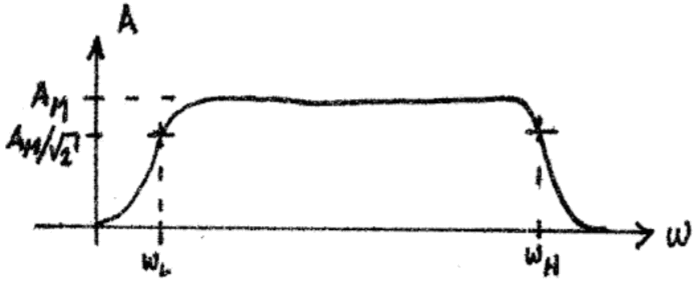
\includegraphics[width=0.9\linewidth]{_fig/respfreq_amp-dc_acomple-c.png}
	\caption{Respuesta de frecuencia del amplificador acoplado capacitivamente}
	\label{fig:respfreq_amp-dc_acomple-c}
\end{figure}

Para la clase de circuito amplificador de banda ancha, una caracterización se distingue por su ganancia a frecuencias medias, $A_m$, y las dos frecuencias esquinas: la frecuencia de corte baja, $f_L$, y la frecuencia de corte alta, $f_H$. Las frecuencias de corte se definen como las frecuencias a las cuales el módulo de la ganancia ha bajado a $1/\sqrt{2}$ de su valor máximo. Alternativamente, se conocen como las frecuencias de media potencia.

Es conveniente considerar la función de transferencia compuesta de la siguiente forma:

\begin{equation}
	A(s) = A_M F_L(s) F_H(s)
\end{equation}

tal como se muestra en la Figura \ref{fig:fig3}. \( A_M \) es la ganancia constante a frecuencias medias; se calcula con los condensadores de acoplamiento y de puente cortocircuitados y sin considerar las limitaciones de frecuencia de los dispositivos. \( F_L(s) \) es la función de \( s \) que encierra todas las dependencias de frecuencia del amplificador a frecuencias bajas y que se caracteriza por un filtro paso alto, es decir:

\[ 
F_L (\omega) \cong 1 \text{ para } \omega \gg \omega_L, \quad F_L(f_L) = 1/\sqrt{2} 
\]

\begin{equation}
	A(s) \cong A_M F_H (s) \text{ para } \omega \gg \omega_L \quad (1.14) 
\end{equation}

\( F_H (s) \) es la función de \( s \) que incluye todos los efectos que afectan la respuesta de frecuencia del amplificador a frecuencias altas y que se caracteriza por un filtro paso bajo, es decir:

\[ 
F_H (\omega) \cong 1 \text{ para } \omega \ll \omega_H, \quad F_H(f_H) = 1/\sqrt{2} 
\]

y

\begin{equation}
	A(s) \cong A_M F_L (s) \text{ para } \omega \ll \omega_H \quad (1.15) 
\end{equation}

\( F_L (s) \) es de la siguiente forma:

\begin{figure}[h]
	\centering
	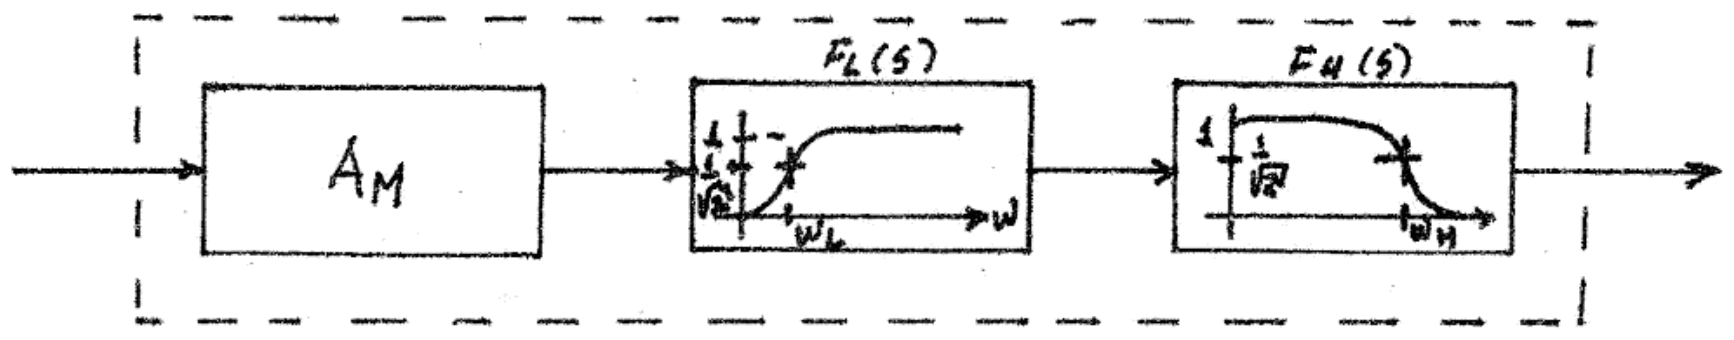
\includegraphics[width=0.9\linewidth]{_fig/respfreq_forma-fl.png}
	\caption{Forma de \( F_L (s) \)}
	\label{fig:respfreq_forma-fl}
\end{figure}

\begin{equation} \label{respfreq_fl}
	F_L(s) = \frac{(s + w_{z1})(s + w_{z2}) \cdots (s + w_{zpn})}{(s + w_{p1})(s + w_{p2}) \cdots (s + w_{pm})}
\end{equation}

donde los \( w_{z1} < w_{p1} \), es decir existen parejas de cero con polo donde la frecuencia del polo es mayor que la frecuencia del cero (filtro paso alto). Además para la relación de la ecuación \ref{respfreq_fl}, cuando \( s \gg w_L \), entonces \( F_L(s) \leq 1 \).

Mientras que \( F_H(s) \) es de la forma:

\begin{equation}
	F_H(s) = \frac{(sT_{z1} + 1)(sT_{z2} + 1)}{(sT_{p1} + 1)(sT_{p2} + 1)} \cdots \frac{(sT_{pn} + 1)}{(sT_{pn} + 1)}
\end{equation}

donde \( T_{p1} > T_{z1} \), es decir la frecuencia del polo es menor que la frecuencia del cero (filtro paso bajo) y generalmente \( T_{z2} = 0 \), y cuando \( s \ll w_H \), \( F_H(s) \leq 1 \).

\section{Análisis de un circuito con FET} %p16

En la Figura \ref{fig:respfreq_amp-fet} se muestra un amplificador FET fuente común con su circuito de polarización, su condensador de acoplamiento a la entrada, \( C_C \), y el condensador de puenteo de la resistencia de la fuente (\( C_S \)).

\begin{figure}[h]
	\centering
	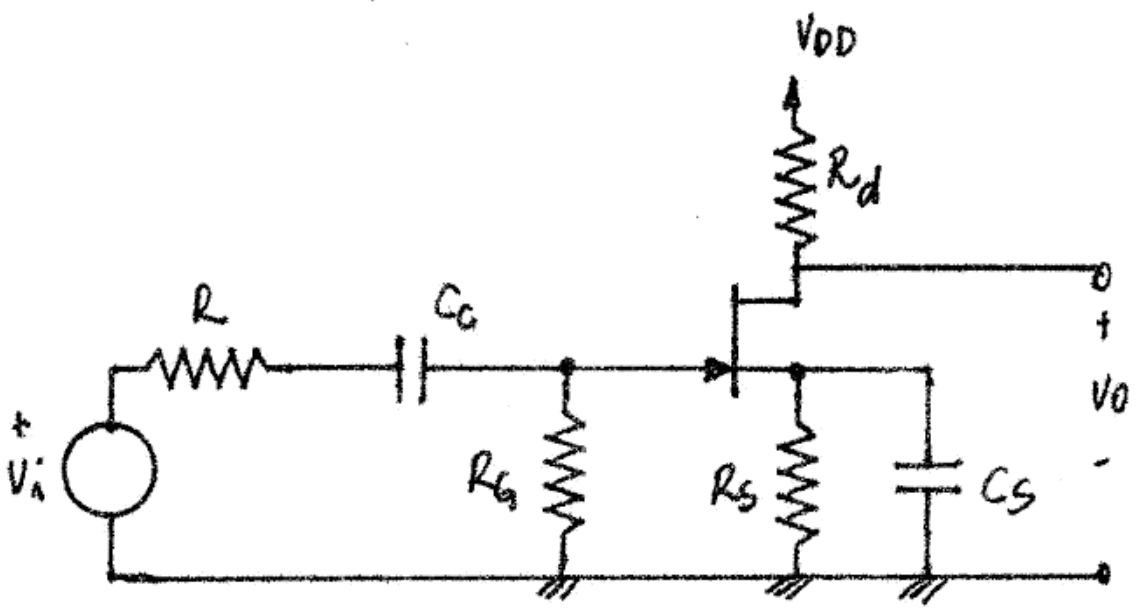
\includegraphics[width=0.9\linewidth]{_fig/respfreq_amp-fet.png}
	\caption{Amplificador FET}
	\label{fig:respfreq_amp-fet}
\end{figure}

El modelo apropiado del FET para realizar nuestro análisis frecuencial se muestra en la Figura \ref{fig:respfreq_modelo-fet}. Además de la fuente de Corriente controlada, \( g_m \psi_{gs} \), y la resistencia de salida, \( r_d \), se incluye capacitancias entre los bornes externos del dispositivo. Para transistores de pequeña señal, estas capacitancias son del orden de los $pF$.

\begin{figure}[h]
	\centering
	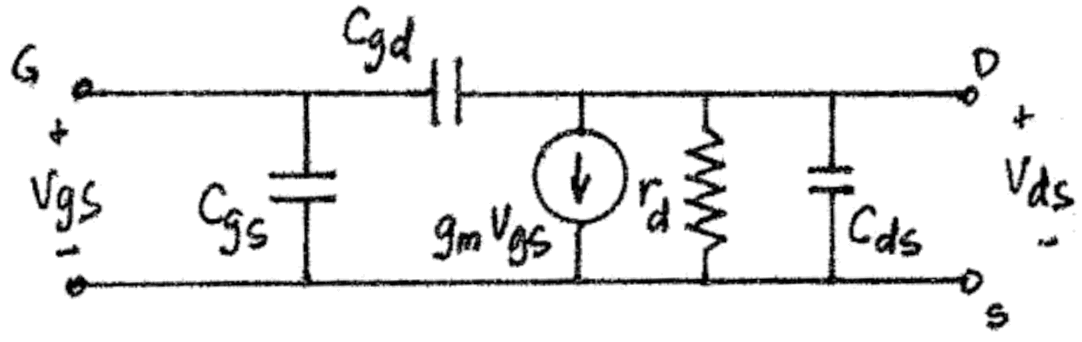
\includegraphics[width=0.9\linewidth]{_fig/respfreq_modelo-fet.png}
	\caption{Modelo del FET}
	\label{fig:respfreq_modelo-fet}
\end{figure}

La forma rutinaria de realizar el análisis frecuencial de este circuito reemplazaría el FET de la Figura \ref{fig:respfreq_amp-fet} con el modelo del FET de la Figura \ref{fig:respfreq_modelo-fet}, resultando así un circuito con 5 condensadores. Es decir, la función de transferencia sería aparentemente una función en $s$ de quinto orden! Y eso que apenas estamos considerando un circuito de un solo transistor. Para circuitos más grandes, cada transistor implica adicionar 3 capacitancias más, sin incluir los condensadores correspondientes de acoplamiento y de puenteo. En fin nos queda por delante un análisis complicado dado lo pequeño que es el circuito.

Como una primera simplificación del análisis, vamos a limitarnos a rangos determinados de frecuencia. Esto ya se hizo cuando se calculó la ganancia \( A_M \) del circuito a frecuencias medias. Haremos un análisis de baja frecuencia en donde no tomaremos en cuenta las capacitancias internas del FET ya que no afectan apreciablemente la respuesta a frecuencias bajas y medias. Y haremos un análisis de alta frecuencia donde no tomaremos en cuenta los condensadores que solo afectan la respuesta a bajas frecuencias.

Antes que nada se debe determinar el punto de operación en continua del circuito, con las ecuaciones:

\begin{equation}
	V_{GS} = V_G - I_D R_S
\end{equation}

\begin{equation}
	I_D = I_{DSS} \left(1 - \frac{V_{GS}}{V_P}\right)^2
\end{equation}

De esta forma podremos calcular el parámetro

\[
g_m = \frac{\partial I_D}{\partial V_{GS}}
\]

Entonces para baja frecuencia se analiza el circuito que se muestra en la Figura \ref{fig:respfreq_modelo-fet-lf}; \( r_d \) no se toma en cuenta por ahora para simplificar el análisis y considerando que su efecto es despreciable. Para mayor precisión se tomaría en cuenta.

\begin{figure}[h]
	\centering
	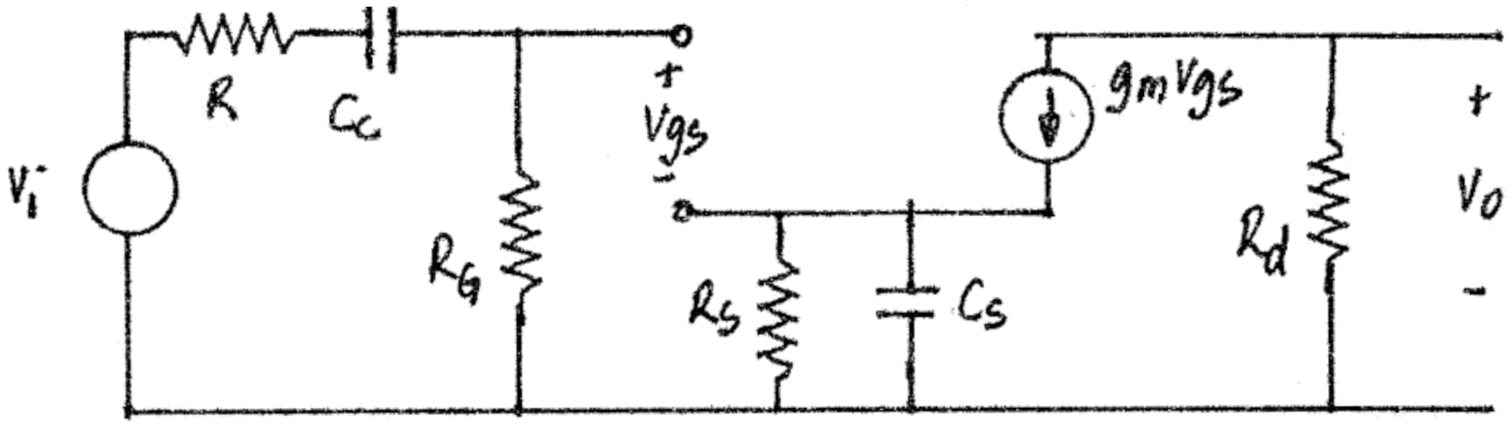
\includegraphics[width=0.9\linewidth]{_fig/respfreq_modelo-fet-lf.png}
	\caption{Modelo del FET para baja frecuencia}
	\label{fig:respfreq_modelo-fet-lf}
\end{figure}

Hallaremos \( \frac{v_o}{v_i'} \) por partes:

\begin{equation}
	\frac{v_o}{v_i'} = \left(\frac{v_o}{v_g}\right) \left(\frac{v_g}{v_i'}\right)
\end{equation}

De la malla de entrada se halla \( \frac{v_g}{v_i'} \):

\[
\frac{v_g}{v_i} = \frac{R_g}{R_g + \frac{1}{sC_C} + R}
\]

\begin{equation} \label{respfreq_vg-vi}
	\frac{v_g}{v_i} = \left(\frac{R_g}{R_g + R}\right) \frac{s}{s + \frac{1}{C_C(R + R_g)}}
\end{equation}

es decir introduce un cero en el origen y un polo a la frecuencia \( -\frac{1}{C_C(R + R_g)} \). Para hallar \( \frac{v_o}{v_g} \), tenemos las siguientes ecuaciones:

\begin{equation}
	v_o = -g_m v_{gs} R_d
\end{equation}

\begin{equation}
	v_{gs} = v_g - v_d
\end{equation}

\begin{equation}
	v_o = -g_m V_{gs} \left( R_s \parallel \frac{1}{C_s s} \right)
\end{equation}

Luego,

\begin{equation} \label{respfreq_vo-vg}
	\frac{v_o}{v_g} = \frac{-g_m R_d \left( s + \frac{1}{R_s C_s} \right)}{s + \frac{1 + 9m R_s}{C_s R_s}}
\end{equation}

Esta parte del circuito nos contribuye un cero en $-1/R_s C_s$, y un polo en $-\frac{1 + 9m R_s}{C_s R_s}$. La relación global es el producto de la ecuación \ref{respfreq_vg-vi} por la ecuación \ref{respfreq_vo-vg}:

\begin{equation}
	\frac{v_o}{v_i} = -\frac{g_m R_d R_q}{R_d + R} \left( \frac{s \left( s + \frac{1}{R_s C_s} \right)}{\left( s + \frac{1}{C_s (R + R_q)} \right) \left( s + \frac{1}{4cm R_s} \right)} \right)
\end{equation}

Esta función tiene la forma $A_M F_L(s)$, donde:

\begin{equation} \label{respfreq_exp_a_m}
	A_M = -\frac{g_m R_d R_q}{R_G + R}
\end{equation}

es la ganancia a frecuencias medias, y

\begin{equation} \label{respfreq_fl-gain-mf}
	F_L(s) = \frac{s \cdot \left( s + \frac{1}{R_s C_s} \right)}{\left( s + \frac{1}{C_s (R + R_q)} \right) \left( s + \frac{1}{4cm R_s} \right)}
\end{equation}

incluye todas las variaciones de frecuencia de la función global para frecuencias bajas. Afortunadamente en este circuito los condensadores se encuentran en mallas independientes de modo que nos resulta expresiones sencillas para las raíces.

Ahora hallaremos la relación $\frac{v_o}{v_i}$ para alta frecuencia. Se cortocircuitan los condensadores de baja frecuencia y nos queda por analizar el circuito que se muestra en la Figura \ref{fig:respfreq_relacion-vo-vi}.

\begin{figure}[h]
	\centering
	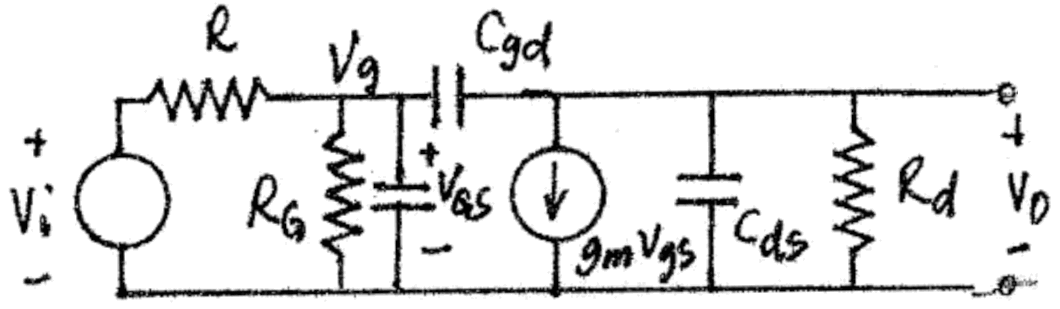
\includegraphics[width=0.9\linewidth]{_fig/respfreq_relacion-vo-vi.png}
	\caption{Modelo del FET para baja frecuencia}
	\label{fig:respfreq_relacion-vo-vi}
\end{figure}

Tenemos las siguientes ecuaciones de nodo:

\begin{equation}
	v_g \left( \frac{1}{R} + \frac{1}{R_q} + s C_{\mathrm{gs}} + s C_{\mathrm{gd}} \right) - v_o s C_{\mathrm{gd}} = \frac{V_i}{R}
\end{equation}

\begin{equation}
	v_g (g_m - sC_{gd}) + v_0(sC_{gd} + sC_{dS} + \frac{1}{R_d}) = 0
\end{equation}

de donde se obtiene:

%\[
%\frac{v_o}{v_i} = \frac{\left(-g_m - sC_{gd}\right)/{r}}{s^2\left( C_{ds} \left( C_{gs} + C_{gd} \right) + C_{gd}C_{gs} \right) + s \left( \left( \frac{1}{R} + \frac{1}{R_g} \right) \left( C_{ds} + C_{gd} + C_{gd}g_m \right) \right)} + \frac{1}{R_d} \left( \frac{1}{R} + \frac{1}{R_g} \right)
%\]

\begin{equation} \label{respfreq_vo-vi-gain-mf}
	\frac{v_o}{v_i} = \frac{\frac{-g_m R_d R_G}{R+R_G} \left(1-\frac{C_{gd}}{g_m} \right) }{ s^2 \left[ \frac{C_{ds}\left(C_{gs}+C_{gd}\right)+C_{gd}C_{gs}}{\frac{1}{R_d}\left(\frac{1}{R}+\frac{1}{R_g} \right)}\right]+s\left[R_d\left(C_{ds}+C_{gd}\right)+\frac{C_{gd}g_{m}R_d}{\frac{1}{R}+\frac{1}{R_g}} \right] + 1}
\end{equation}

Esta expresión está de la forma \(p_{ij}(s)\), donde:

\[
A_{M} = -\frac{g_m R_d R_G}{R + R_G}
\]

tiene la misma expresión de la ecuación \ref{respfreq_exp_a_m}, y

\begin{equation} \label{respfreq_funcion-transferencia}
	F_H(s) = \frac{1 - \frac{sC_{gd}}{g_M}}{s^2 \left[ \frac{C_{ds}\left(C_{gs}+C_{gd}\right)+C_{gd}C_{gs}}{\frac{1}{R_d}\left(\frac{1}{R}+\frac{1}{R_G}\right)} \right] + s\left[ R_d\left(C_{ds}+C_{gd}\right)+\frac{C_{gd}g_{m}R_{d}}{\frac{1}{R}+\frac{1}{R_{G}}} \right] + 1}
\end{equation}

La ganancia a frecuencias medias es lo que queda de la ecuación \ref{respfreq_vo-vi-gain-mf} para \(s\) relativamente pequeña. La ecuación \ref{respfreq_vo-vi-gain-mf} es una función de segundo orden cuyos polos pueden resolverse utilizando la solución cuadrática. No queda una función de tercer orden pues las tres capacitancias forman un lazo. Lo que sí puede apreciarse es que los polos no son funciones simples de condensadores individuales, ya que estos interactúan.

Ahora podemos unir los resultados de las ecuaciones \ref{respfreq_fl-gain-mf} y \ref{respfreq_vo-vi-gain-mf} para plantear a continuación la función de transferencia total del circuito de la Figura \ref{fig:respfreq_amp-fet}:

\begin{equation}
	\frac{v_o}{v_i}= \frac{-g_m R_d R_G}{R_G + R} F_{L}(S) F_{H} (S)
\end{equation}

\subsubsection{Ejemplo 1} \label{respfreq_ejm1}

Para el circuito de la Figura \ref{fig:respfreq_amp-fet} se tiene los siguientes valores: \(R_G = 1M\Omega \), \(R = 100k\Omega \), \(R_d = 2.2k\Omega\), \(R_s = 1k\Omega\), \(V_{DD} = 10V\), \(C_c = 0.1\mu F\), \(C_s = 10\mu F \). Para el FET se tiene \(I_{DSS} = 4mA\), \( V_p = -2V \), \( C_{gd} = 2pF \), \( C_ds = 3pF \), \( C_{gs} = 1pF \).

\textbf{a)} Hallar la función de transferencia del circuito, que corresponde a la ecuación \ref{respfreq_funcion-transferencia}.

\textbf{b)} Trazas el Diagrama de Bode correspondiente.

\textbf{Solución:}

\textbf{a)} Punto de operación: \( V_{gs} = -1V \), \( I_D = 1mA \), \( g_m = 2 mmho \)

\[
A_M = -4
\]

\[
F_L(s) = \frac{s(s + 100)}{(s + 9.09)(s + 300)}
\]

\[
F_H(s) = \frac{(1 - 10^{-9}s)}{(7.34 \times 10^{-7}s + 1)(2.72 \times 10^{-9}s + 1)}
\]

Con lo que la función global queda:
\[
\frac{v_o}{v_i} = \frac{-4s(s + 100)(1 - 10^{-9}s)}{(s + 9.09)(s + 300)(7.34 \times 10^{-7}s + 1)(2.72 \times 10^{-9}s + 1)}
\]

\textbf{b)} Trazar el Diagrama de Bode correspondiente:

Ver figura \ref{fig:respfreq_graph-ejemplo}

\begin{figure}[h]
	\centering
	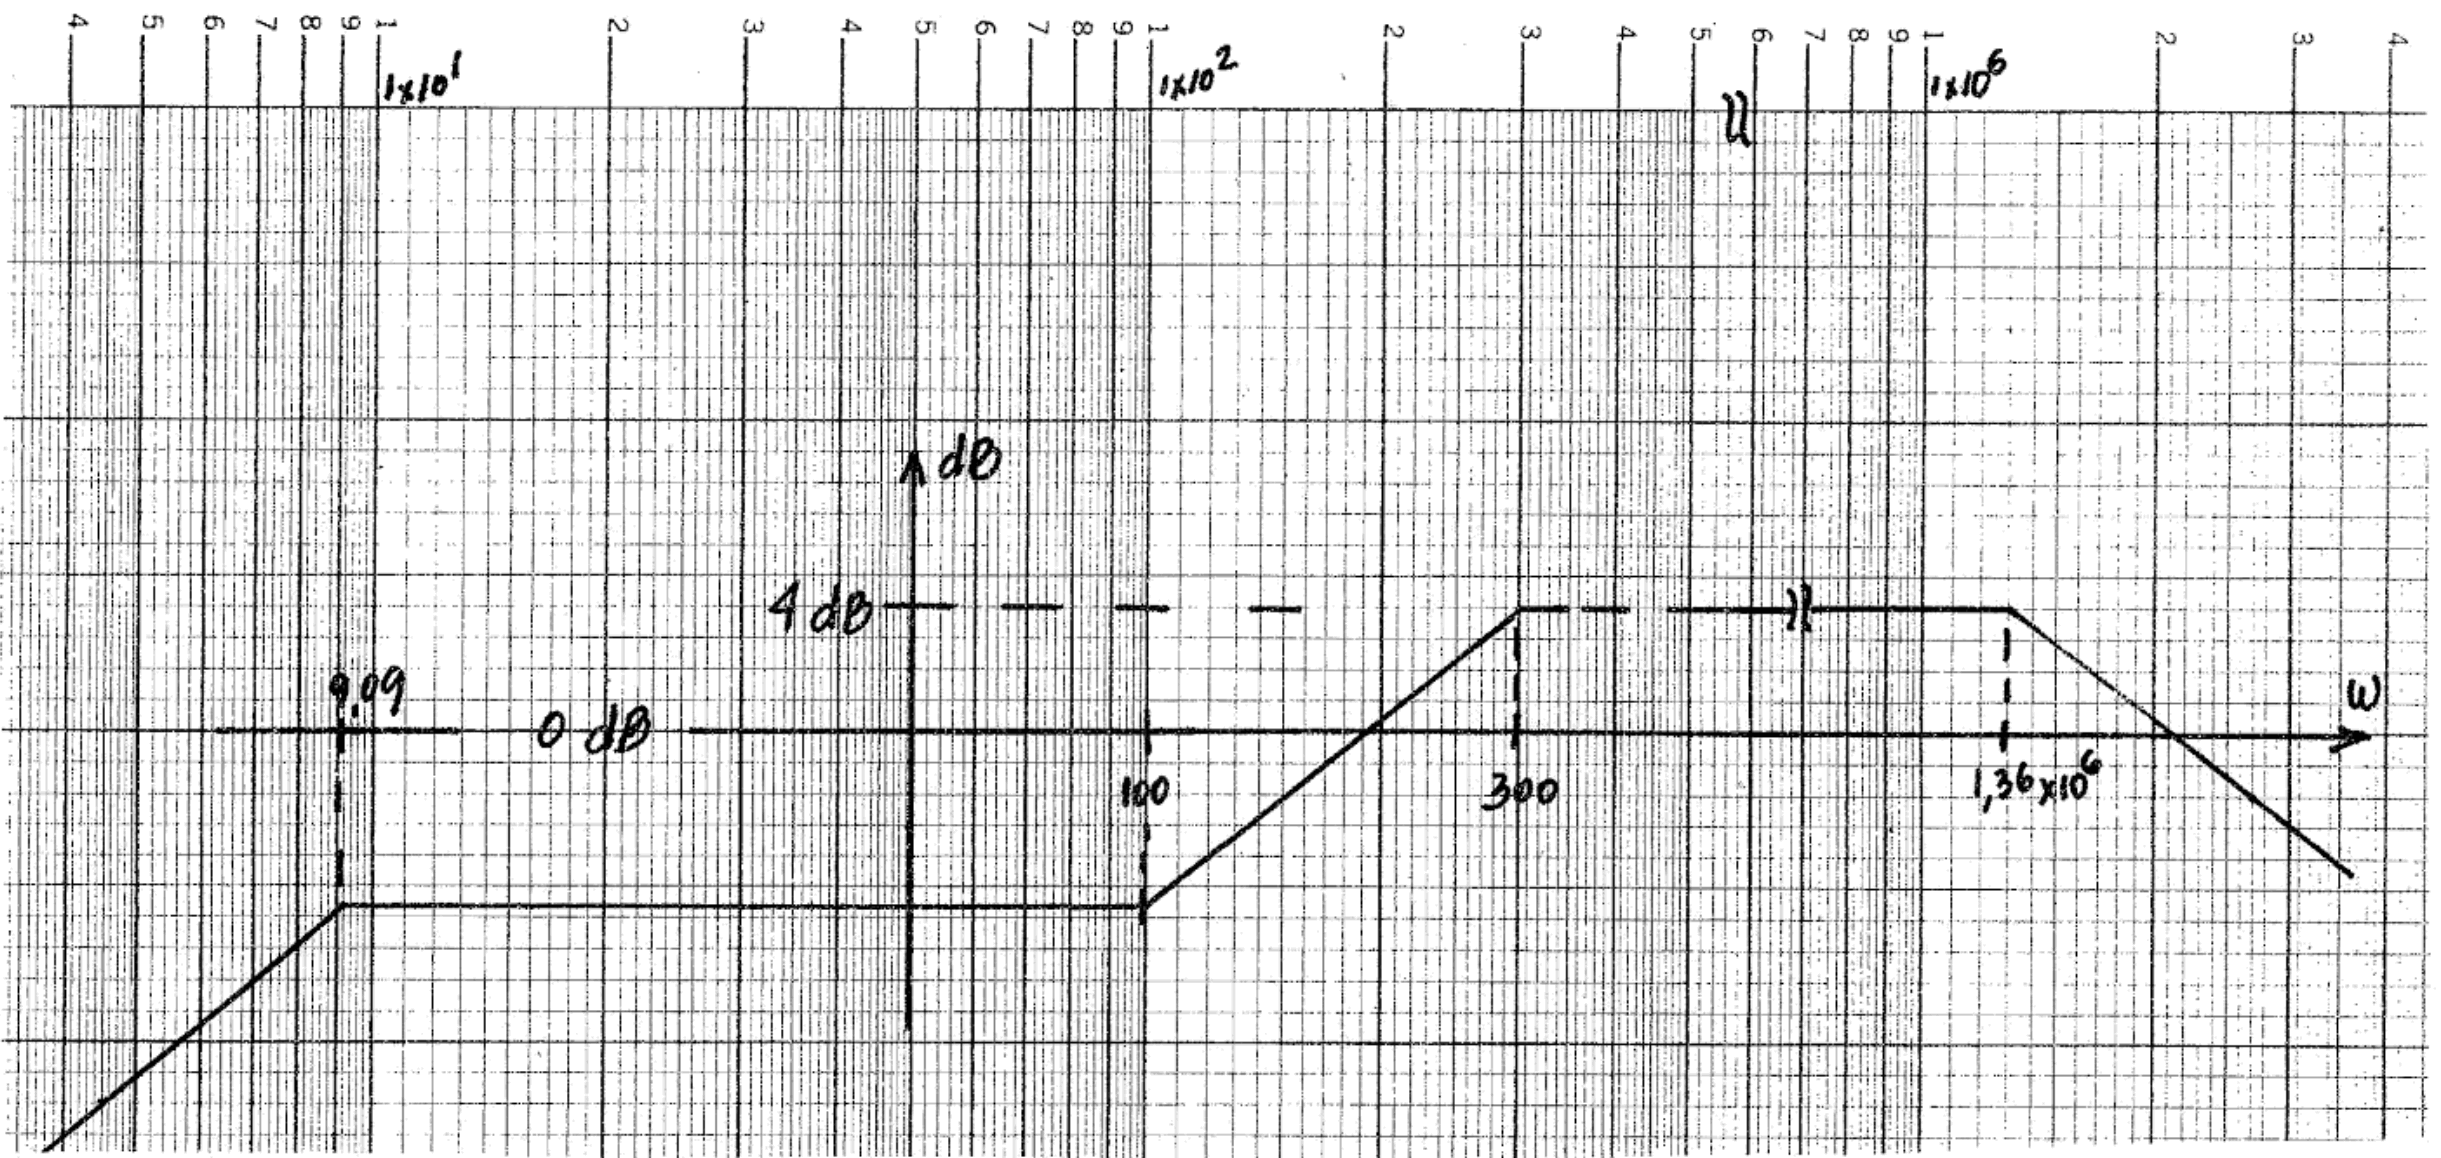
\includegraphics[width=0.9\linewidth]{_fig/respfreq_graph-ejemplo.png}
	\caption{Diagrama de Bode resultante (ejemplo)}
	\label{fig:respfreq_graph-ejemplo}
\end{figure}


\section{Método de Superposición} %p21
En la sección anterior se planteó un amplificador sencillo con FET que resultó tener una función de transferencia de cuarto orden. Se pudo simplificar el análisis en parte al despreciar el efecto de ciertos componentes según el rango de frecuencia. De ésta forma quedaban circuitos más sencillos para resolver. Sin embargo, incluso con esta simplificación, determinar la función de transferencia resultó engorroso, un problema que se agrava en circuitos más grandes. Esto representa un desafío en sistemas electrónicos complejos, compuestos frecuentemente por múltiples etapas. Programas como \textit{SPICE}, \textit{ECAP} y \textit{MICROCAP} pueden analizar redes de hasta 50 nodos, pero su enfoque numérico no identifica los componentes críticos en la función de transferencia.

Para efectos de diseño y de un análisis crudo de un circuito, lo que hace falta es un método sencillo que permita estimar las frecuencias de corte o de esquina y saber que componentes influyen en cada frecuencia de esquina. Vamos a aprovechar que conocemos la respuesta típica de un amplificador, como las que aparecen en las figuras \ref{fig:respfreq_amp-dc} y \ref{fig:respfreq_amp-dc_acomple-c}, para caracterizar simplemente con su valor de ganancia a frecuencias medias, una frecuencia de corte alta y una frecuencia de corte baja. Así se puede plantear la función de transferencia, aunque sea en forma aproximada. Por lo tanto presentamos el Método de Superposición. Con él vamos a encontrar una expresión de las raíces correspondientes a cada elemento reactivo en forma independiente. Después su efecto quedará reflejado en la frecuencia de corte baja o la frecuencia de corte alta.

El método consiste en los siguientes pasos. En primer lugar, clasificar los elementos reactivos (capacitancias e inductancias) según formen parte de \( F_L(s) \) o \( F_H(s) \):

\begin{itemize}
	\item Si el elemento actúa como filtro paso alto, pertenece a \( F_L(s) \) (elemento de \textit{baja frecuencia}).
	\item Si actúa como filtro paso bajo, pertenece a \( F_H(s) \) (elemento de \textit{alta frecuencia}).
\end{itemize}

Por ejemplo, los condensadores de acople y puenteo son de baja frecuencia, mientras las capacitancias internas del dispositivo son de alta frecuencia.

\subsection{Procedimiento para frecuencias bajas}

Se trabaja con el circuito de frecuencias bajas (condensadores de alta frecuencia como circuitos abiertos) para hallar la frecuencia de corte baja global:

\begin{enumerate}
	\item[\textbf{a)}] Cortocircuitar todos los condensadores excepto uno, \( C_K \). Calcular:
	\begin{itemize}
		\item Polo asociado:
		\begin{equation}
			\omega_{PK} = \frac{1}{R_R C_K}
		\end{equation}
		donde \( R_R \) es la resistencia de Thevenin vista desde \( C_K \).
		\item Cero asociado:
		\begin{equation}
			\omega_{ZK} = \frac{1}{R_R C_K}
		\end{equation}
		donde \( R_R \) es la resistencia en paralelo con \( C_K \).
	\end{itemize}
	
	\item[\textbf{b)}] Repetir el paso (a) para los demás condensadores de baja frecuencia.
	
	\item[\textbf{c)}] La función \( F_L(s) \) aproximada es:
	\begin{equation}
		F_L(s) = \frac{(s + \omega_{Z1})(s + \omega_{Z2}) \cdots (s + \omega_{Zm})}{(s + \omega_{P1})(s + \omega_{P2}) \cdots (s + \omega_{Pm})}
	\end{equation}
	y la frecuencia de corte baja global (\( \omega_L \)) se obtiene como:
	\[
	\omega_L = \sum_{k=1}^{m} \omega_{Pk}
	\]
\end{enumerate}

\subsection{Procedimiento para frecuencias altas}

Se analiza el circuito de frecuencias altas (condensadores de baja frecuencia como cortocircuitos):

\begin{enumerate}
	\item[\textbf{a)}] Dejar abiertos todos los condensadores excepto uno, \( C_k \). Calcular su polo asociado:
	\begin{equation}
		\omega_{Pk} = \frac{1}{R_k C_k}
	\end{equation}
	donde \( R_k \) es la resistencia de Thévenin vista desde \( C_k \). El cero se supone en \( \omega \to \infty \).
	
	\item[\textbf{b)}] Repetir el paso (a) para los demás condensadores de alta frecuencia.
	
	\item[\textbf{c)}] La función \( F_H(s) \) aproximada es:
	\begin{equation}
		F_H(s) = \frac{1}{\left(1 + \sum_{i=1}^n \frac{s}{\omega_{Pi}}\right)\left(1 + \sum_{j=1}^n \frac{s}{\omega_{Pj}}\right)\left(1 + \sum_{k=1}^n \frac{s}{\omega_{Pk}}\right)}
	\end{equation}
	\textit{Nota: La formulación original contiene sumatorias sin términos, posible error tipográfico.}
	
	La frecuencia de corte alta global es:
	\begin{equation}
		\omega_H = \frac{1}{\sum_{i=1}^n \frac{1}{\omega_{Pi}}}
	\end{equation}
\end{enumerate}

\subsection{Procedimiento para frecuencias medias}

Se calcula con condensadores de baja en corto y alta en abierto:

\begin{equation}
	A(s) = A_M \frac{1}{\left(1 + \frac{\omega_L}{s}\right)} \frac{1}{\left(1 + \frac{s}{\omega_H}\right)}
\end{equation}

\subsubsection{Ejemplo 2} \label{respfreq_ejm2}
Repita el ejemplo 1.1 utilizando este procedimiento.

\textbf{Solución:}

\textbf{Análisis de Baja Frecuencia:}

Utilice el circuito de la Figura \ref{fig:respfreq_modelo-fet-lf}

\begin{itemize}
	\item Para \( C_c \), \(R_p = \infty \):
	\[
	R_{Th} = 100k \Omega + 1M \Omega = 1.1M \Omega
	\]
	y la contribución a la función de transferencia:
	\[
	\frac{s}{s + \frac{1}{(0.1 \times 10^{-7}) \cdot 1.1 \times 10^6}} = \frac{s}{s + 9.09}
	\]
	
	\item Para \( C_s \), \( R_p = R_s \) :
	Se encuentra \( R_{Th} \) apoyado en la Figura \ref{fig:respfreq_sch-ejemplo2}.
	\begin{figure}[h]
		\centering
		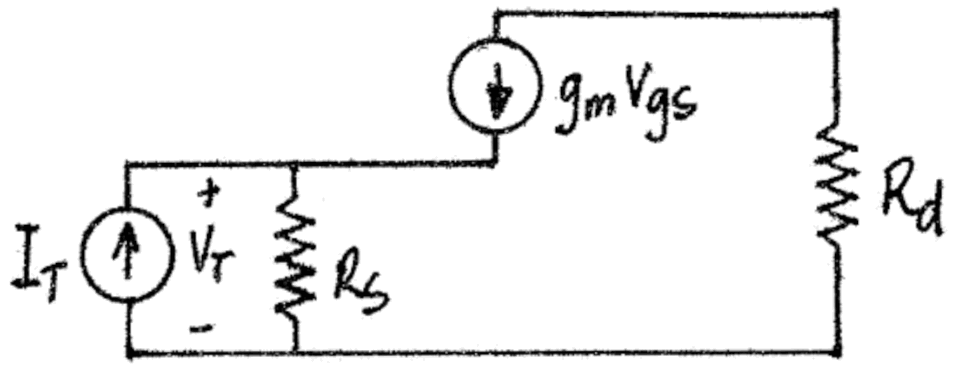
\includegraphics[width=0.9\linewidth]{_fig/respfreq_sch-ejemplo2.png}
		\caption{Circuito equivalente}
		\label{fig:respfreq_sch-ejemplo2}
	\end{figure}
	Se tiene:					
	\[
	I_T = \frac{V_T}{R_s} - g_m v_{gs}
	\]
	pero
	\[
	v_{gs} = -V_g - V_s ; V_g=0 ; V_s = V_t
	\]
	entonces
	\[
	v_{gs} = -V_T
	\]
	de donde
	\[
	I_T = V_T \left( g_m + \frac{1}{R_s} \right)
	\]
	y
	\[
	R_{Th} = \frac{V_T}{I_T} = \frac{1}{g_m + \frac{1}{R_s}} = \frac{R_s}{1 + g_m R_s}
	\]
	y su contribución a la función de transferencia:
	\[
	\frac{s + \frac{1}{C_s R_s}}{s + \frac{1 + g_m R_s}{C_s R_s}} = \frac{s + 100}{s + 300}
	\]
	y la función de transferencia de baja frecuencia queda:
	\[
	F_L(s) = \frac{s(s + 100)}{(s + 9.09)(s + 300)}
	\]
	aquí \(F_L(s)\) coincide con el resultado de \(F_L(s) \) del ejemplo 1.1. Esto no siempre se cumple y se da en éste caso por el hecho de que \( C_c \) y \( C_s \) se encuentran en mallas independientes.
\end{itemize}

\textbf{Análisis de Alta Frecuencia:}

Utilizando el circuito de la Figura \ref{fig:respfreq_relacion-vo-vi}

Para \( C_{gs} \): \( R_{Th} = 1M\Omega \parallel 100k\Omega = 90.9k\Omega \) y \( w_{cgs} = \frac{1}{90.9k \times 10^{-12}} = 1.1 \times 10^7 \)

Para \( C_{gs} \): \( R_{Th} = R_d = 2.2k \Omega \) ; la fuente \( g_m v_{gs} \) desaparece ya que la malla de entrada no llega señal, todas las tensiones en esa malla son cero, particularmente la que controla la fuente de corriente; por lo tanto la fuente de corriente es cero y se convierte en un circuito abierto.

Para \( C_{gd} \), se encuentra \( R_{Th} \) apoyado en la Figura \ref{fig:respfreq_sch-ejemplo2_c_gd}:

\begin{figure}[h]
	\centering
	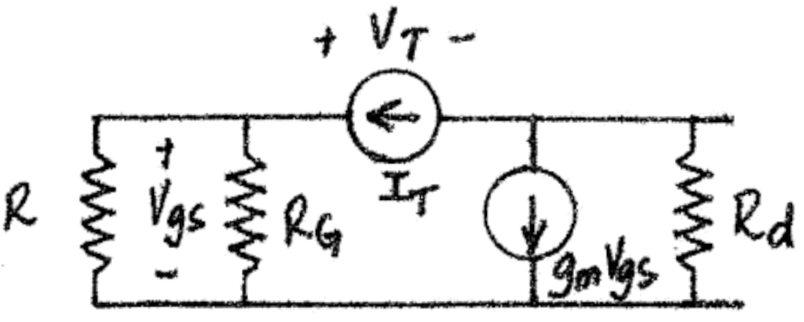
\includegraphics[width=0.9\linewidth]{_fig/respfreq_sch-ejemplo2_c_gd.png}
	\caption{ Circuito equivalente para \( C_{gd} \)}
	\label{fig:respfreq_sch-ejemplo2_c_gd}
\end{figure}

Se tiene:
\[
V_T = v_{gs} + I R_d
\]
donde \( I = g_m v_{gs} + I_T \), ademas
\[
v_{gs} = I_T (R \parallel R_G)
\]
entonces
\[
V_T = I_T \left( R \parallel R_G + g_m (R \parallel {R_g R_d}) + R_d \right)
\]
y
\[
R_h = R \parallel R_g + g_m (R \parallel { R_g R_d })  + R_d = 493k\Omega
\]
y
\[
\omega_{gd} = \frac{1}{493k\Omega 2pF} = 1.01 \times 10^6 rad/s
\]
luego
\[
\omega_H = \frac{1}{\frac{1}{1.01 \times 10^6} + \frac{1}{1.1 \times 10^7} + \frac{1}{1.52 \times 10^8}} = 923 krad/s
\]


\section{Comparación entre el método de superposición y el método exacto} %p26

Implícito en el Método de Superposición hay dos aproximaciones:

\begin{enumerate}
	\item la primera admite determinar por separado la contribución de cada elemento reactivo a la respuesta de frecuencia, cuando en realidad habrá una interacción si comparten una malla o nodo.
	\item el cálculo de las frecuencias de corte baja y alta, tal como aparecen en las ecuaciones (1.36) y (1.39).
\end{enumerate}

Generalmente el efecto de colocar en cascada a varias etapas es el de aumentar la frecuencia de corte inferior del conjunto y disminuir la frecuencia de corte superior. En la Figura 1.22 se muestra una cascada de $N$ filtros paso altos, cada uno con frecuencia de corte.

\begin{figure}[h]
	\centering
	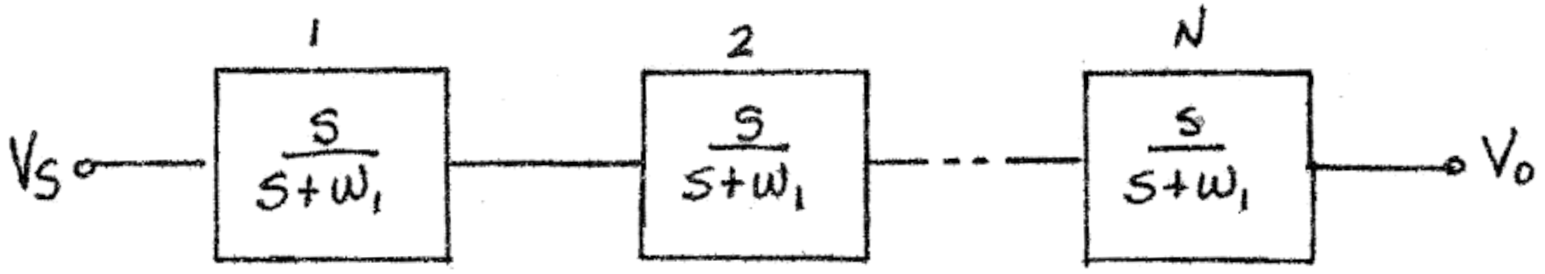
\includegraphics[width=0.9\linewidth]{_fig/respfreq_cascada-n-hp-filters.png}
	\caption{Cascada de $N$ filtros paso alto}
	\label{fig:respfreq_cascada-n-hp-filters}
\end{figure}

La función de transferencia viene dada por:

\begin{equation}
	\frac{V_o}{V_s}(s) = \frac{s^N}{(s+\omega_1)^N}
\end{equation}

Esta función tiene un valor de uno para $s$ elevada; por lo tanto, la frecuencia de media potencia, \( \omega_L \), viene dada por:

\begin{equation}
	\left| \frac{(j\omega_L)^N}{(j\omega_L + \omega_1)^N} \right| = \frac{1}{\sqrt{2}}
\end{equation}

Luego,

\[
\left[1 + \left(\frac{\omega_1}{\omega_L}\right)^2 \right]^{N/2} = 2^{1/2}
\]

\begin{equation} \label{respfreq_hp-fmp}
	\omega_L = \omega_1 \sqrt{2^{1/N} -1}
\end{equation}

Se hace notar que la raíz $N$ de $2$ da como resultado un número entre $1$ y $2$, por lo que $\omega_L$ es siempre mayor que $\omega_1$.

En forma semejante, para una cascada de $N$ filtros paso bajo con función $1/(sT_A + 1)$, la frecuencia de corte alta para la función total, $\frac{V_o}{V_s} = 1/(sT_A +1)^N$, viene dada por:

\begin{equation} \label{respfreq_hp-fc-ft}
	\omega_H = \omega_A \sqrt{2^{1/N}-1}, \quad \omega_A = \frac{1}{T_A}
\end{equation}

Es decir, la cascada de filtros de este tipo tiene el efecto de disminuir la frecuencia de corte alta. Se puede extender este análisis a un sistema filtro paso banda de banda ancha,

\[
\left(\frac{s}{s+\omega_1} \right) \left(\frac{1}{sT_A+1} \right)
\]

que se grafica en la Figura \ref{fig:respfreq_analisis-pasa-banda}.

\begin{figure}[h]
	\centering
	\subfloat[Filtro Paso Banda]
	{
		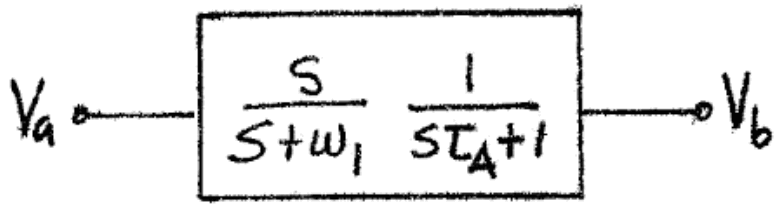
\includegraphics[width=0.4\linewidth]{_fig/respfreq_analisis-pasa-banda-filtro.png}
		\label{fig:respfreq_analisis-pasa-banda-filtro}
	}
	\subfloat[Respuesta del Módulo]
	{
		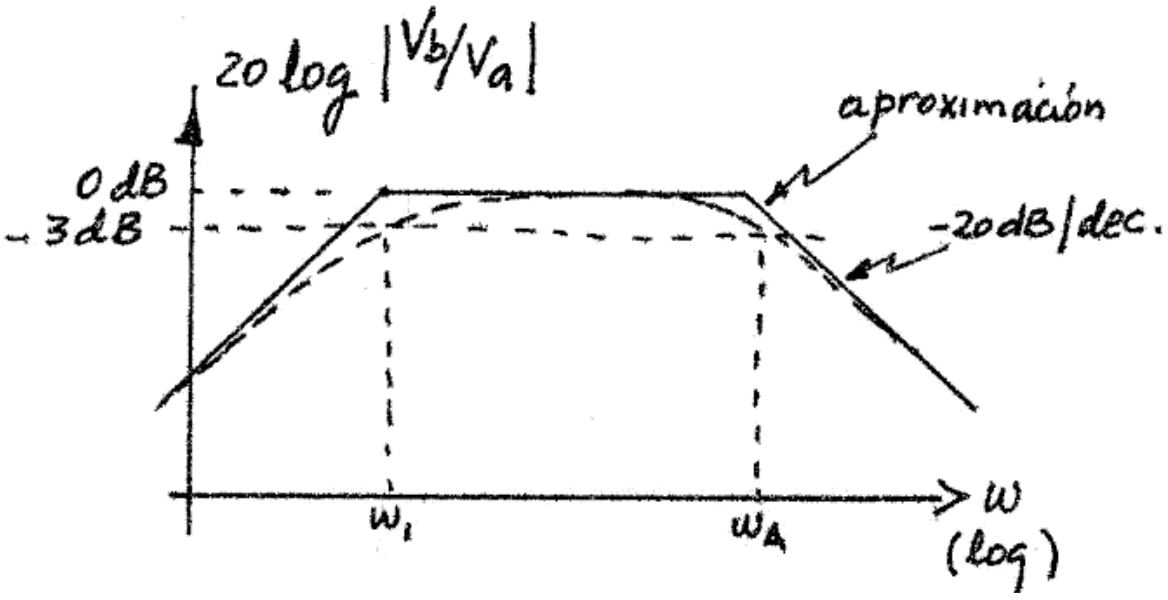
\includegraphics[width=0.4\linewidth]{_fig/respfreq_analisis-pasa-banda-resp.png}
		\label{fig:respfreq_analisis-pasa-banda-resp}
	}
	\caption{Modelo de un Amplificador Operacional con su Respuesta de Frecuencia}
	\label{fig:respfreq_analisis-pasa-banda}
\end{figure}

Al colocar dos bloques de este tipo en cascada, se consigue la función de transferencia del sistema:

\begin{equation}
	\frac{V_o}{V_s}(s) = \left[ \frac{s}{s+\omega_1} \cdot \frac{1}{sT_A+1} \right]^2
\end{equation}

La gráfica de esta función se puede trazar a partir de la Figura \ref{fig:respfreq_analisis-pasa-banda-resp}. Cada bloque tendrá esta respuesta, y el efecto de los dos es equivalente a la suma de dos de estas gráficas: el resultado se observa en la Figura \ref{fig:respfreq_analisis-pasa-banda-resp2}.

\begin{figure}[h]
	\centering
	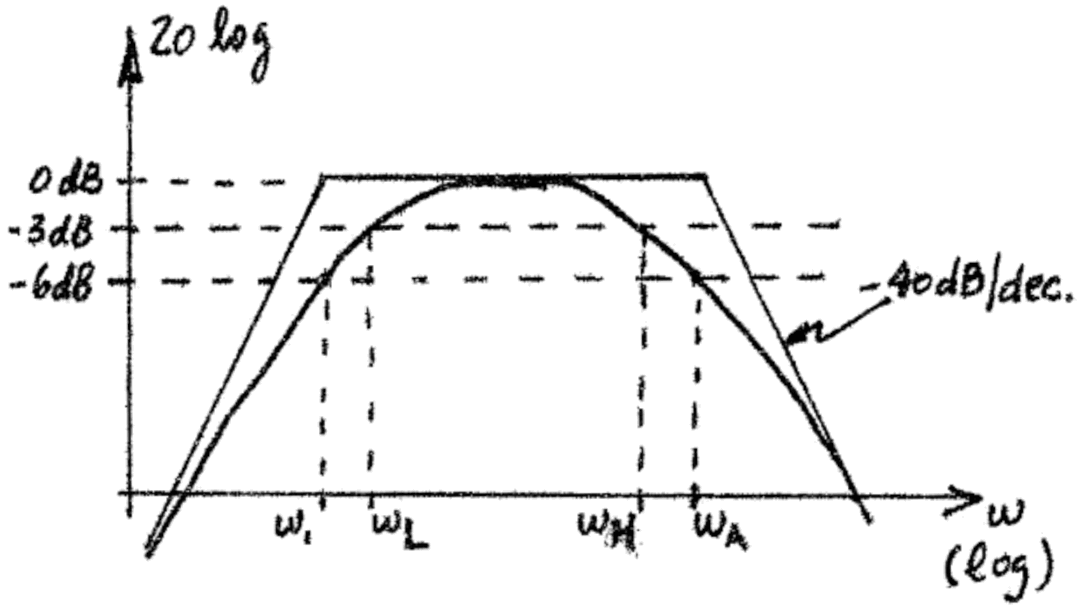
\includegraphics[width=0.8\linewidth]{_fig/respfreq_analisis-pasa-banda-resp2.png}
	\caption{Respuesta equivalente}
	\label{fig:respfreq_analisis-pasa-banda-resp2}
\end{figure}

Las asíntotas tienen valores de $+40$ dB/década por el lado de abajo debido al efecto del doble cero en el origen, y de $-40$ dB/década por el lado de arriba debido al doble polo a la frecuencia de $\omega_A$.

A las frecuencias de $\omega_1$ y $\omega_A$, la ganancia es $-6$ dB. De la curva real se puede observar que las frecuencias de media potencia, cuando la ganancia ha bajado $3$ dB, se han corrido. La frecuencia de corte baja, $\omega_L$, es mayor que la frecuencia de una etapa, $\omega_1$, y la frecuencia de corte alta, $\omega_H$, es menor que la de una etapa. El ancho de banda total es menor que el ancho de banda de una etapa.

Si los polos de alta y baja frecuencia son muy distantes, aún se cumplen las ecuaciones \ref{respfreq_hp-fmp} y \ref{respfreq_hp-fc-ft}:

\begin{itemize}
	\item Para $n=2$:
	\[
	\omega_L = \omega_1 / \sqrt{2^{1/2}-1} = 1.55\omega_1
	\]
	\[
	\omega_H = \omega_A \sqrt{2^{1/2}-1} = 0.644\omega_A
	\]
	\item Para $n=3$:
	\[
	\omega_L = \omega_1 / \sqrt{2^{1/3}-1} = 1.96\omega_1
	\]
	\[
	\omega_H = \omega_A \sqrt{2^{1/3}-1} = 0.51\omega_A
	\]
\end{itemize}

¿Qué ocurre en los casos donde las etapas no tienen las mismas frecuencias de corte? Condición que se indica en las figuras \ref{fig:respfreq_comp-metodo_ejm1-diagrama}, \ref{fig:respfreq_comp-metodo_ejm1-resp-1b2b} y \ref{fig:respfreq_comp-metodo_ejm1-resp-total}.

\begin{figure}[h]
	\centering
	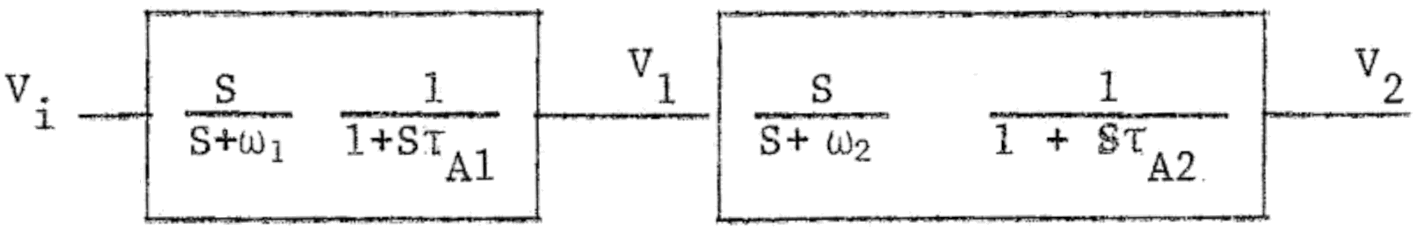
\includegraphics[width=0.9\linewidth]{_fig/respfreq_comp-metodo_ejm1-diagrama.png}
	\caption{Ejemplo: Diagrama de bloque}
	\label{fig:respfreq_comp-metodo_ejm1-diagrama}
\end{figure}

\begin{figure}[h]
	\centering
	\subfloat[Respuesta primer bloque]
	{
		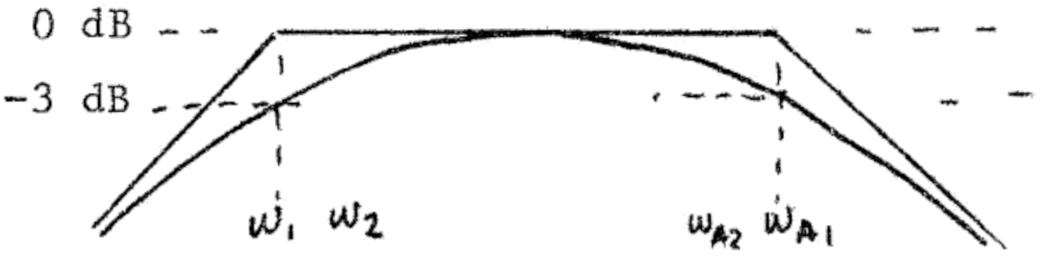
\includegraphics[width=0.4\linewidth]{_fig/respfreq_comp-metodo_ejm1-resp-1b.png}
		\label{fig:respfreq_comp-metodo_ejm1-resp-1b}
	}
	\subfloat[Respuesta segundo bloque]
	{
		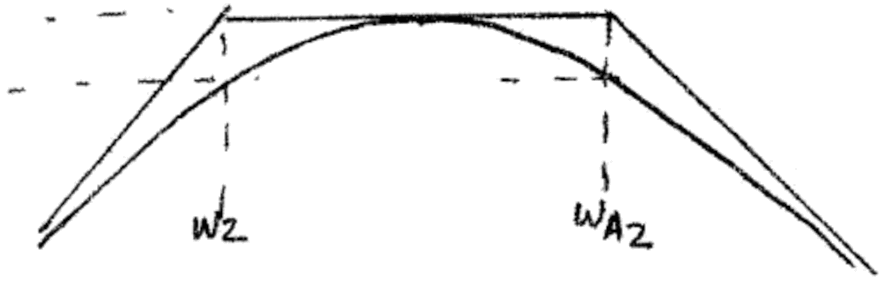
\includegraphics[width=0.4\linewidth]{_fig/respfreq_comp-metodo_ejm1-resp-2b.png}
		\label{fig:respfreq_comp-metodo_ejm1-resp-2b}
	}
	\caption{Ejemplo: Respuestas primer y segundo bloque}
	\label{fig:respfreq_comp-metodo_ejm1-resp-1b2b}
\end{figure}

\begin{figure}[h]
	\centering
	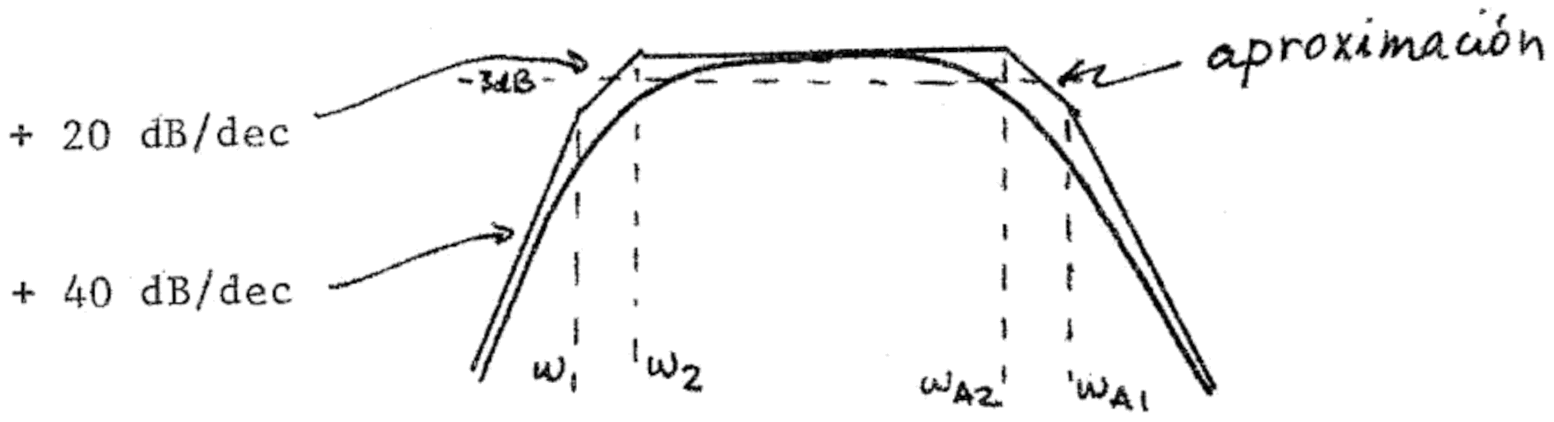
\includegraphics[width=0.9\linewidth]{_fig/respfreq_comp-metodo_ejm1-resp-total.png}
	\caption{Ejemplo: Respuesta total}
	\label{fig:respfreq_comp-metodo_ejm1-resp-total}
\end{figure}

La frecuencia de $-3$ dB tiene que ser:

\begin{description}
	\item[a.] por el lado bajo mayor que \( \omega_2 \)
	\item[b.] por el lado alto menor que \( \omega_A2 \)
\end{description}

Para los casos en que \( \omega_2 \gg \omega_1 \), entonces la frecuencia de corte inferior: \( \omega_L \approx \omega_2 \), y si \( \omega_{A2} \ll \omega_{A1} \) entonces la frecuencia de corte superior: \( \omega_H \approx \omega_{A2} \). Estos son los casos de \textbf{polo dominante}. Cuando las etapas no tienen frecuencias de corte iguales, la etapa con la frecuencia de corte más hacia el centro de la banda de paso es la que predomina en la determinación de la frecuencia de corte del conjunto.

A continuación se encuentra la expresión exacta de la frecuencia de corte superior para el caso de:

\[
G(s) = \frac{1}{(1+s/\omega_1)(1+s/\omega_2)}
\]

Por definición:

\[
G(\omega_H) = \frac{1}{\sqrt{2}} = \left| \frac{1}{1 + j\frac{\omega_H}{\left(\frac{\omega_1 + \omega_2}{2}\right)} + \frac{(j\omega_H)^2}{\omega_1\omega_2}} \right|
\]

de donde:

\begin{equation} \label{respfreq_equ-dificil}
	\omega_H^2 = -\frac{(\omega_1^2 + \omega_2^2)}{2} \pm \sqrt{\frac{(\omega_1^2 + \omega_2^2)^2}{4} + (\omega_1\omega_2)^2}
\end{equation}

\subsubsection{Ejemplo 3} \label{respfreq_ejm3}

\textbf{a)} Para \( \omega_1 = 10^6 \), \( \omega_2 = 10^6 \), se obtiene \( \omega_H = 643K \), resultado que se espera de acuerdo con la ecuación (1.44).

\textbf{b)} Para \( \omega_1 = 10^6 \), \( \omega_2 = 10^6 \), se obtiene \( \omega_H = 990K \), se hace notar la cercanía de \( \omega_H \) a \( \omega_2 \) para \( \omega_1 \gg \omega_2 \).

Es relativamente laborioso llegar a la expresión de la ecuación \ref{respfreq_equ-dificil}. Se puede imaginar lo complicado que sería determinar la expresión general de \( \omega_H \) para el caso de tres polos. Siempre se puede acudir a un computador para conseguir la solución. Sin embargo, conviene el Método de Superposición.

\section{Un enfoque distinto para graficar el diagrama de Bode del módulo} %p31

Generalmente, la función de transferencia de un amplificador se expresa como se hizo en la ecuación (1.13), que repetimos a continuación:

\[
G(s) = A_M F_L(s) F_H(s)
\]

Uno puede trazar el Diagrama de Bode del módulo sin necesidad de trazar las contribuciones individuales de las raíces. Partimos de la ganancia \( A_M \), que se convierte en nuestro punto de referencia y de allí se traza el resto del diagrama.

Por ejemplo, si 

\[
G(s) = A_M \frac{(s + \omega_1) \omega_3}{(s + \omega_2)(s + \omega_3)}
\]

\begin{equation} \label{respfreq_bodealt-eq}
	G(s) = A_M \frac{(s + \omega_1)}{(s + \omega_2)(sT_3 + 1)}
\end{equation}

donde: \( T_3 = \frac{1}{\omega_3} \); entonces \( F_L(s) = \frac{s + \omega_1}{s + \omega_2}\), \( F_H(s) = \frac{1}{sT_3 + 1}	\) y \( \omega_3 \gg \omega_2 > \omega_1 \), en la Figura \ref{fig:respfreq_bodealt} se trazan los efectos de cada una de estas componentes progresivamente hasta llegar al resultado final, la Figura \ref{fig:respfreq_bodealt-d}.

\begin{figure}[h]
	\centering
	\subfloat[A]
	{
		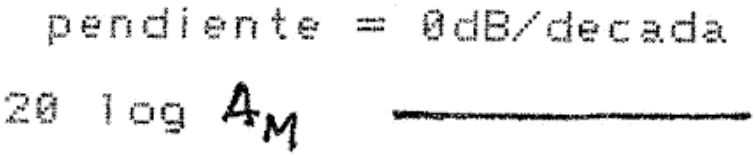
\includegraphics[width=0.2\linewidth]{_fig/respfreq_bodealt-a.png}
		\label{fig:respfreq_bodealt-a}
	}
	\subfloat[B]
	{
		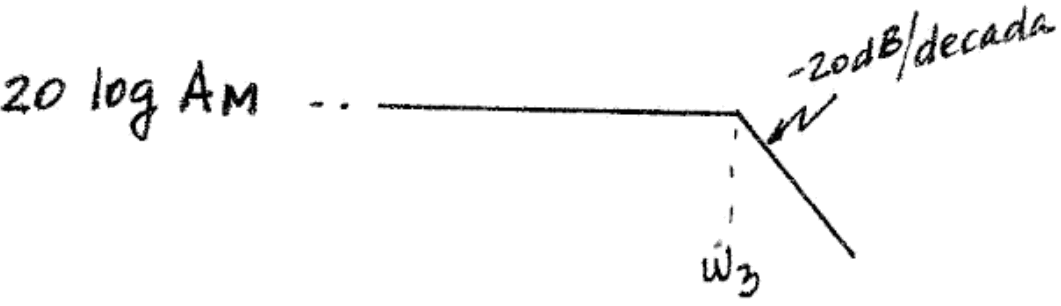
\includegraphics[width=0.32\linewidth]{_fig/respfreq_bodealt-b.png}
		\label{fig:respfreq_bodealt-b}
	}
	\subfloat[C]
	{
		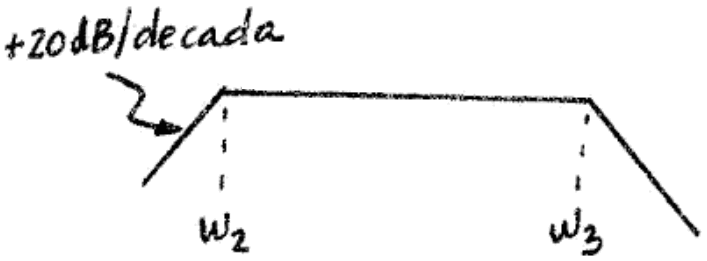
\includegraphics[width=0.2\linewidth]{_fig/respfreq_bodealt-c.png}
		\label{fig:respfreq_bodealt-c}
	}
	\subfloat[D]
	{
		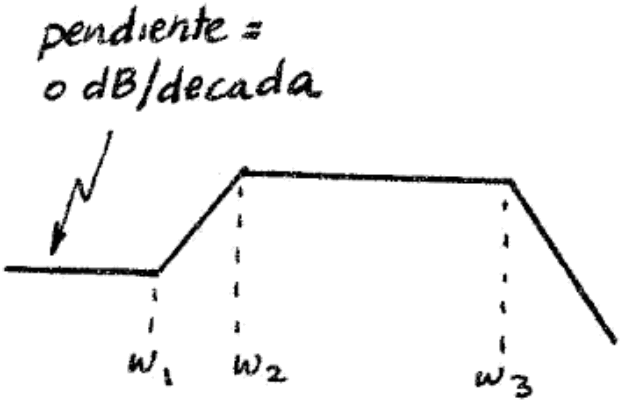
\includegraphics[width=0.2\linewidth]{_fig/respfreq_bodealt-d.png}
		\label{fig:respfreq_bodealt-d}
	}
	\caption{Ejemplo: Traza de ejemplo, Diagrama de Bode}
	\label{fig:respfreq_bodealt}
\end{figure}

Un recorrido detallado de como se analiza la Figura \ref{fig:respfreq_bodealt} es como sigue:
\begin{itemize}
	\item La ganancia a frecuencias medias es \( 20 \log A_M \), ver Figura \ref{fig:respfreq_bodealt-a}.
	\item A partir de \( \omega_3 \) comienza una pendiente de \( -20 dB/decada \) (efecto de un polo de alta frecuencia), ver Figura \ref{fig:respfreq_bodealt-b}.
	\item Desplazándonos hacia la izquierda, el polo en \( \omega_2 \) deja de contribuir su pendiente de \(-20 dB/decada \) en \( \omega_2 \), lo que resulta en una pendiente de \( +20 dB/decada \), ver Figura \ref{fig:respfreq_bodealt-c}.
	\item Desplazándonos aún más a la izquierda alcanzamos el \textbf{cero} en \( \omega_1 \); este deja de contribuir su pendiente de \( +20 dB/decada \) en \( \omega_1 \), ¡y la pendiente cambia por un valor de \( -20 dB/decada \), es decir, cambia a una pendiente de \( 0 dB/decada \), ver Figura \ref{fig:respfreq_bodealt-d}.
\end{itemize}






Funciones más complicadas se trazan utilizando el mismo enfoque.

\section{La respuesta de frecuencia de circuitos con transistores BJT} %p32

\begin{figure}[h]
	\centering
	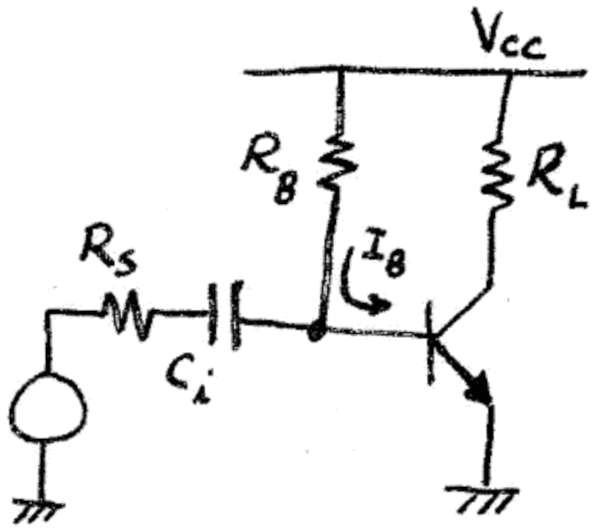
\includegraphics[width=0.35\linewidth]{_fig/respfreq_bjt-base.png}
	\caption{Amplificador emisor común}
	\label{fig:respfreq_bjt-base}
\end{figure}

Analizamos el amplificador emisor común de la Figura \ref{fig:respfreq_bjt-base}.

La resistencia \( R_B \) suministra el camino para la corriente de base de polarización. Hace falta un capacitor de acoplo \( C_i \) para desacoplar en corriente continua (c.c.) la señal de entrada de la base del transistor, evitando que se perturbe el punto de operación y permitiendo el acoplamiento en corriente alterna (c.a.).

Para corriente continua, el circuito equivalente se muestra en la Figura \ref{fig:respfreq_bjt-analisis-cc}. Este circuito se usa para determinar el punto de reposo del transistor y verificar si se encuentra en la región activa. 

Para corriente alterna, el análisis se basa en la Figura \ref{fig:respfreq_bjt-analisis-ca}, donde las fuentes de continua desaparecen: las fuentes de tensión se representan como cortocircuito y las fuentes de corriente como circuito abierto.


Y reemplazando el transistor por un modelo de la región activa, el resultado se muestra en la Figura \ref{fig:respfreq_bjt-analisis-modelo}, se presenta el modelo del transistor, el cual incluye los parámetros \( h_{fe} \) y la transconductancia \( g_m V_i \), permitiendo analizar el comportamiento del circuito en señales pequeñas.

\begin{figure}[h]
	\centering
	\subfloat[A]
	{
		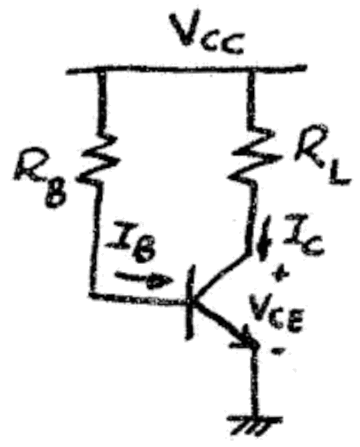
\includegraphics[width=0.15\linewidth]{_fig/respfreq_bjt-analisis-cc.png}
		\label{fig:respfreq_bjt-analisis-cc}
	}
	\subfloat[B]
	{
		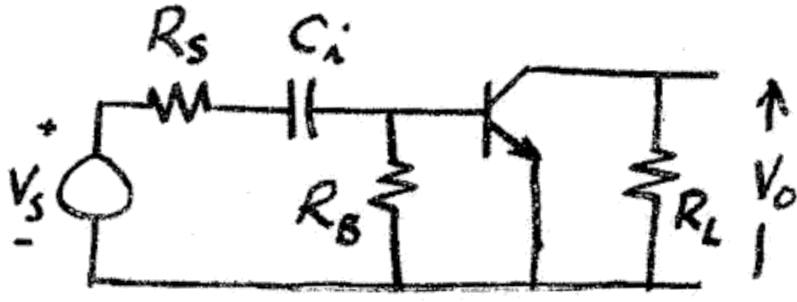
\includegraphics[width=0.25\linewidth]{_fig/respfreq_bjt-analisis-ca.png}
		\label{fig:respfreq_bjt-analisis-ca}
	}
	\subfloat[C]
	{
		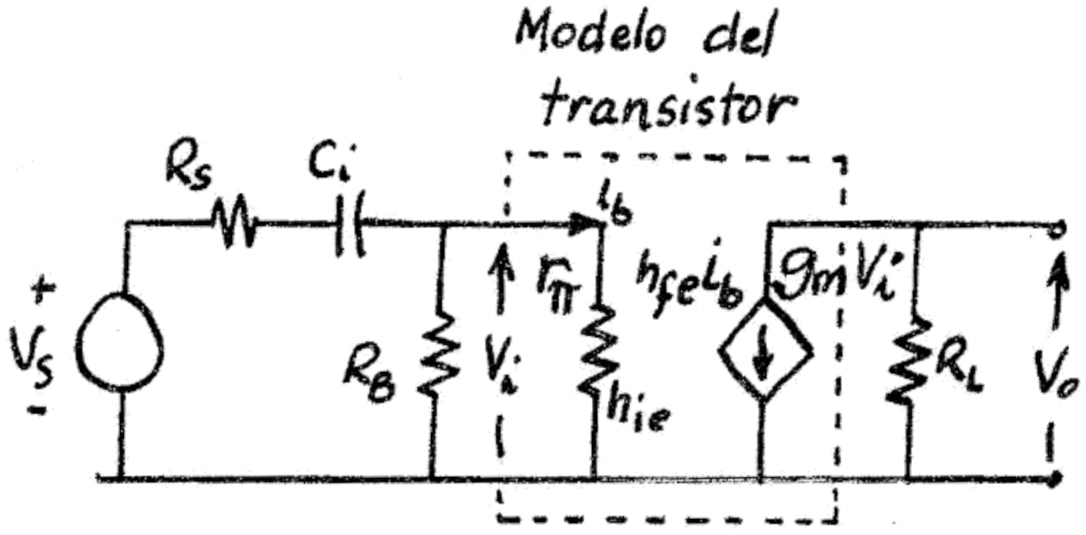
\includegraphics[width=0.5\linewidth]{_fig/respfreq_bjt-analisis-modelo.png}
		\label{fig:respfreq_bjt-analisis-modelo}
	}
	\caption{Analizando amplificador emisor común}
	\label{fig:respfreq_bjt-analisis}
\end{figure}

A frecuencias medias, la reactancia del condensador se hace despreciable y el circuito queda como se muestra en la Figura \ref{fig:respfreq_bjt-frecuencias-medias}.

\begin{figure}[h]
	\centering
	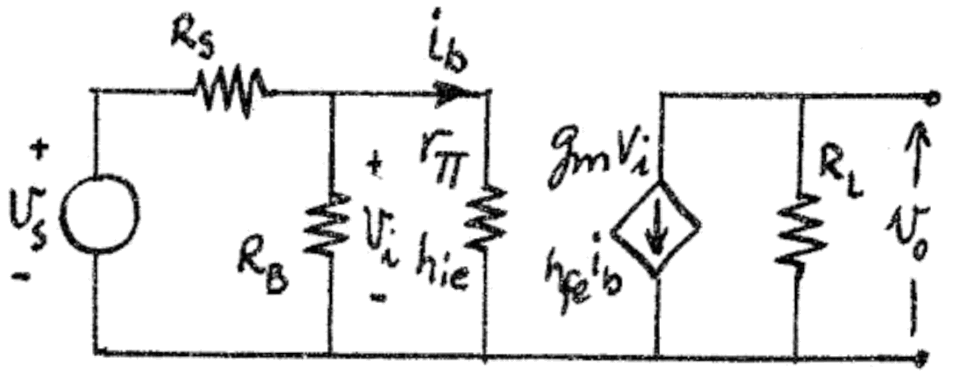
\includegraphics[width=0.6\linewidth]{_fig/respfreq_bjt-frecuencias-medias.png}
	\caption{Modelo del transistor a frecuencias medias}
	\label{fig:respfreq_bjt-frecuencias-medias}
\end{figure}

Con este circuito se obtienen los valores a frecuencias medias de la ganancia de voltaje \( A_V \), de corriente \( A_I \), la resistencia de entrada \( R_i \) y de salida \( R_o \):

\[
V_o = - g_m V_i R_L
\]

\[
V_i = \frac{R_B \parallel r_{\pi}}{R_B \parallel r_{\pi} + R_S} V_S
\]

Por lo que la ganancia de voltaje es:

\begin{equation}
	\frac{V_o}{V_S} = \frac{- g_m R_L (R_B \parallel r_{\pi})}{R_B \parallel r_{\pi} + R_S}
\end{equation}

Para conseguir la función de transferencia \( \frac{V_o}{V_S}(s) \), volvemos a la Figura \ref{fig:respfreq_bjt-analisis-modelo} consideramos que:

\begin{equation}
	\frac{V_i}{V_S} = \frac{R_B \parallel r_{\pi}}{R_B \parallel r_{\pi} + \frac{1}{C_i s} + R_S} = \frac{R_B \parallel r_{\pi}}{R_B \parallel r_{\pi} R_S} \frac{s}{s + \frac{1}{C_i (R_S + R_B \parallel r_{\pi})}}
\end{equation}

Luego:

\begin{equation} \label{respfreq_bjt-ft}
	\frac{V_o}{V_S} = \frac{- g_m R_L (R_B \parallel r_{\pi})}{R_B \parallel r_{\pi} + R_S} \frac{s}{s + \frac{1}{C_i (R_S + R_B \parallel r_{\pi})}}
\end{equation}

Esto muestra la presencia de un cero y un polo en la función de transferencia, afectando la respuesta en frecuencia del circuito.

La función está expresada en la forma de la Ecuación \ref{respfreq_bodealt-eq}. Se grafica la respuesta de frecuencia en la Figura \ref{fig:respfreq_bjt-respfreq}. Se hace notar que el: \( polo = -\frac{1}{C_i (R_S + R_B \parallel r_{\pi})} = -\frac{1}{C_i R_T}	\) donde \( R_T \) es la resistencia de Thevenin vista desde los bornes de \( C_i \).

\begin{figure}[h]
	\centering
	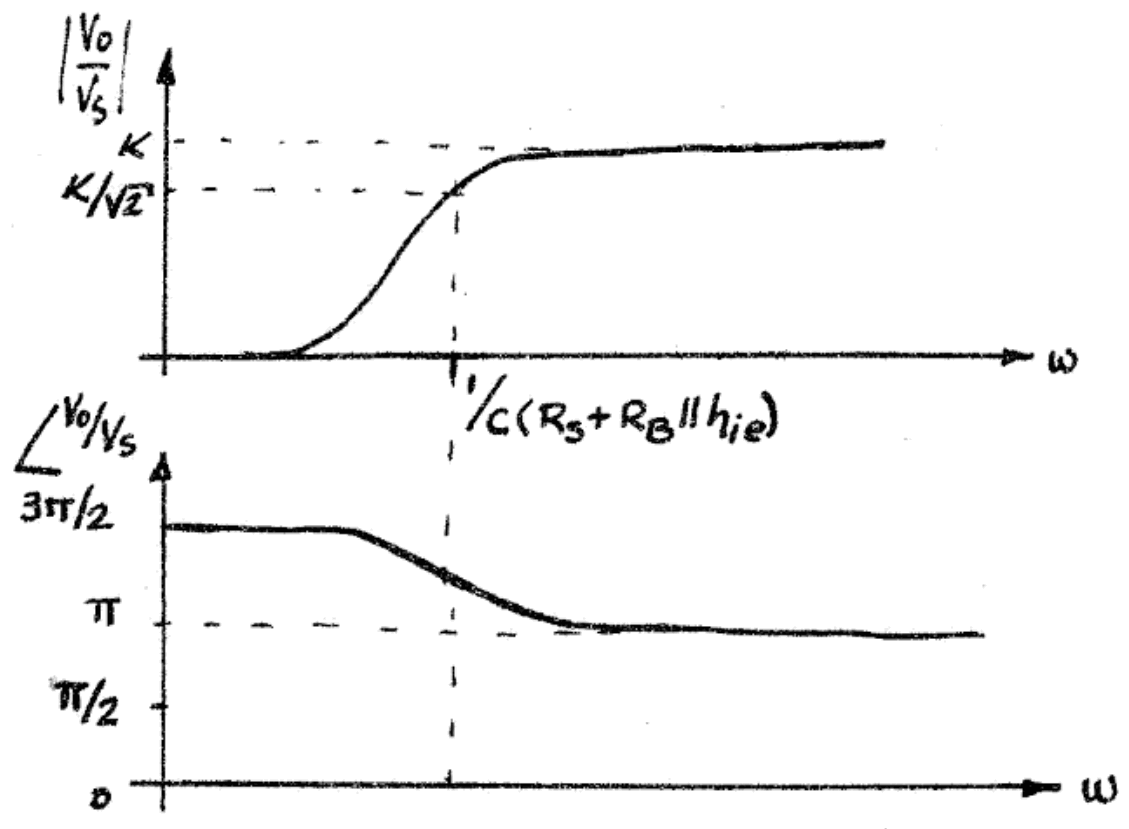
\includegraphics[width=0.6\linewidth]{_fig/respfreq_bjt-respfreq.png}
	\caption{Respuesta de frecuencia del circuito de la Figura \ref{fig:respfreq_bjt-base}}
	\label{fig:respfreq_bjt-respfreq}
\end{figure}

Dado el circuito de la Figura 1.27, los valores de \( r_{\pi} \) y \( \beta \) se encuentran en función del punto de operación sobre las características de entrada y salida del transistor, como se muestra en la Figura \ref{fig:respfreq_bjt-inout}.

\begin{figure}[h]
	\centering
	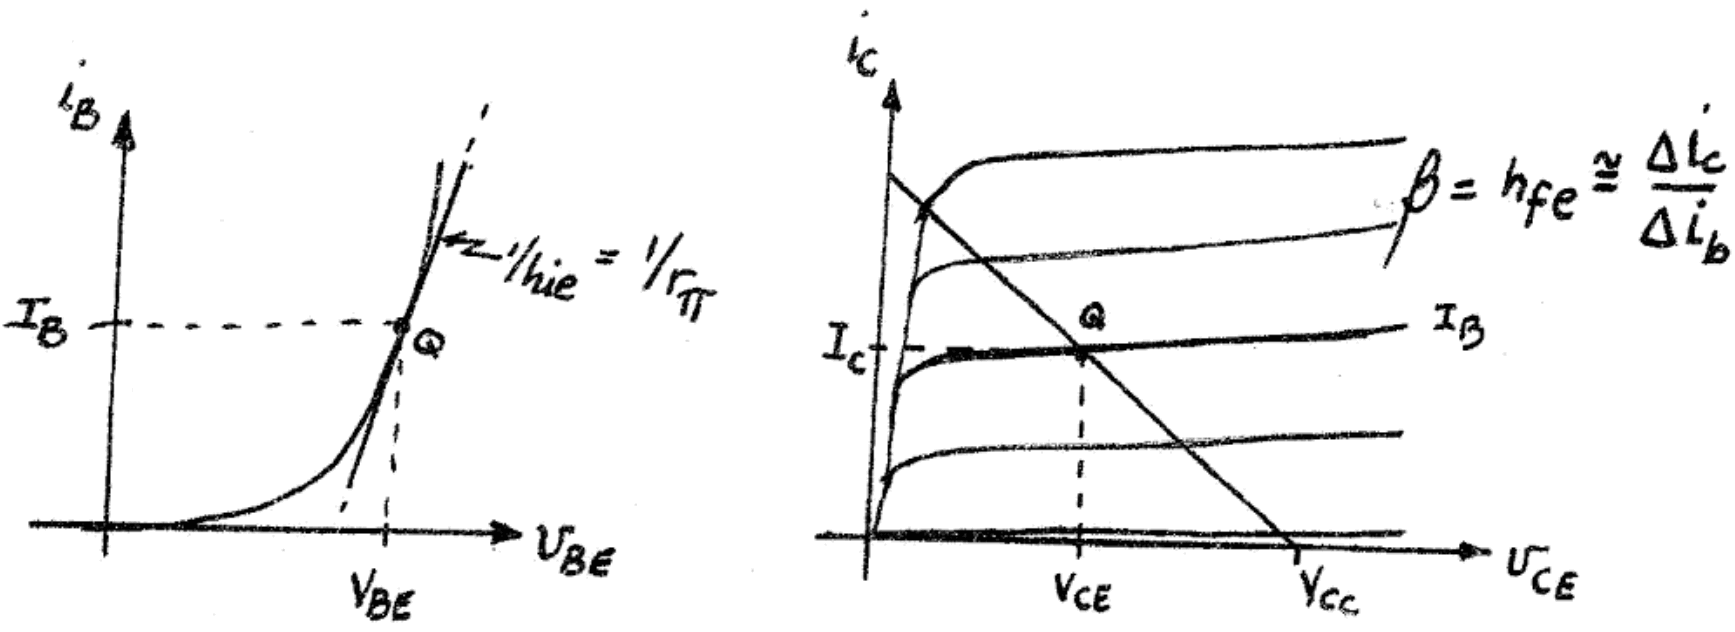
\includegraphics[width=0.6\linewidth]{_fig/respfreq_bjt-inout.png}
	\caption{Características de entrada y salida del transistor}
	\label{fig:respfreq_bjt-inout}
\end{figure}

En el circuito de la Figura \ref{fig:respfreq_bjt-con-cap-a}, se acopla una carga \( R_C \) capacitivamente al colector del transistor del circuito de la Figura \ref{fig:respfreq_bjt-base}. El cambio de la recta de carga se muestra en la Figura \ref{fig:respfreq_bjt-rectas-de-carga}.

\begin{figure}[h]
	\centering
	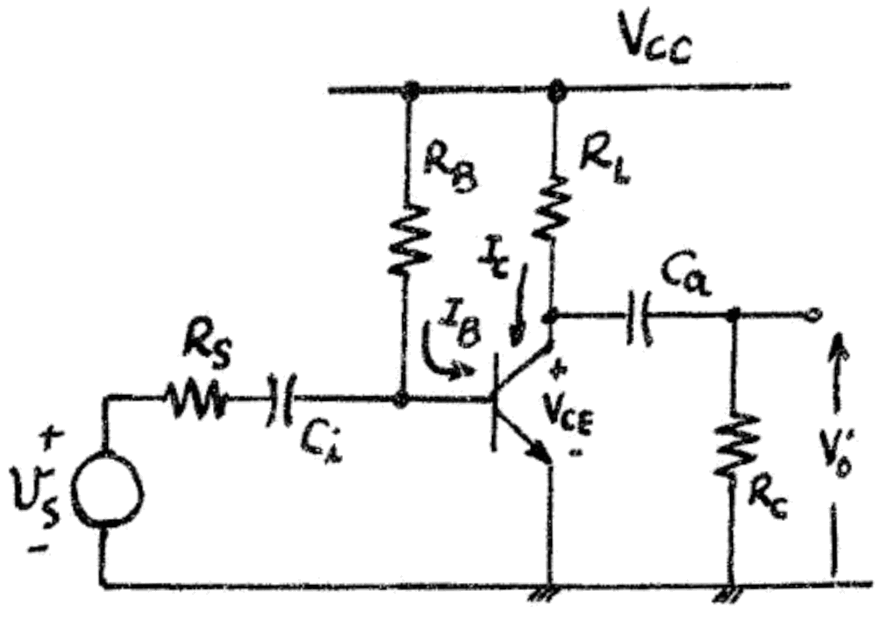
\includegraphics[width=0.5\linewidth]{_fig/respfreq_bjt-con-cap-a.png}
	\caption{Circuito con capacitancia \( C_a \)}
	\label{fig:respfreq_bjt-con-cap-a}
\end{figure}

\begin{figure}[h]
	\centering
	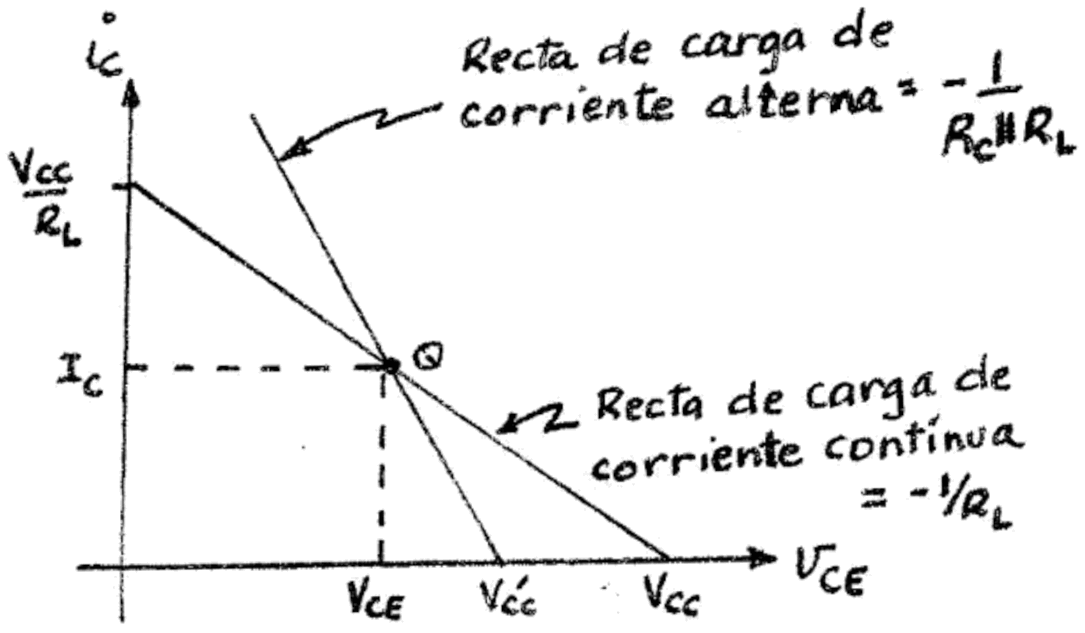
\includegraphics[width=0.6\linewidth]{_fig/respfreq_bjt-rectas-de-carga.png}
	\caption{Rectas de carga de c.a. y c.a. del circuito de la Figura \ref{fig:respfreq_modelo-fet-lf}}
	\label{fig:respfreq_bjt-rectas-de-carga}
\end{figure}

Para hallar la relación de \( \frac{V_o}{V_s} \), apenas hace falta hallar la relación \( \frac{V_o}{V_i}(s) \), pues ya encontramos la relación \( \frac{V_i}{V_s} \).

\subsection{Red de Salida para Corriente Alterna}

El circuito correspondiente se plantea en la Figura \ref{fig:respfreq_bjt-red-salida-ca}.

\begin{figure}[h]
	\centering
	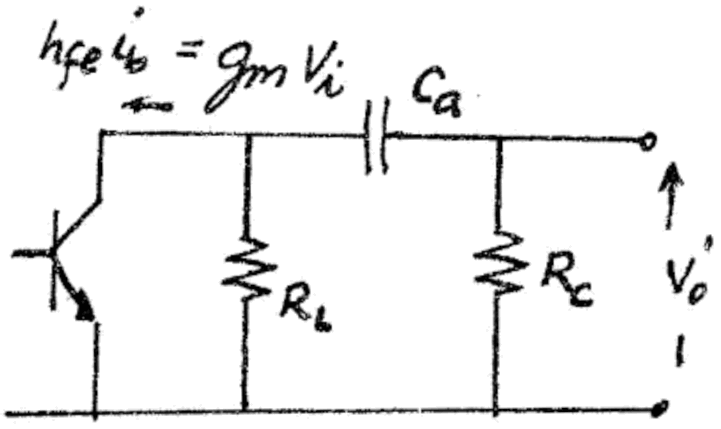
\includegraphics[width=0.5\linewidth]{_fig/respfreq_bjt-red-salida-ca.png}
	\caption{Red de salida para corriente alterna}
	\label{fig:respfreq_bjt-red-salida-ca}
\end{figure}

Reemplazando el transistor por su modelo y transformando la combinación de la fuente de corriente y \( R_L \) en su equivalente de Thevenin, nos queda la Figura \ref{fig:respfreq_bjt-eq-thevenin}.

\begin{figure}[h]
	\centering
	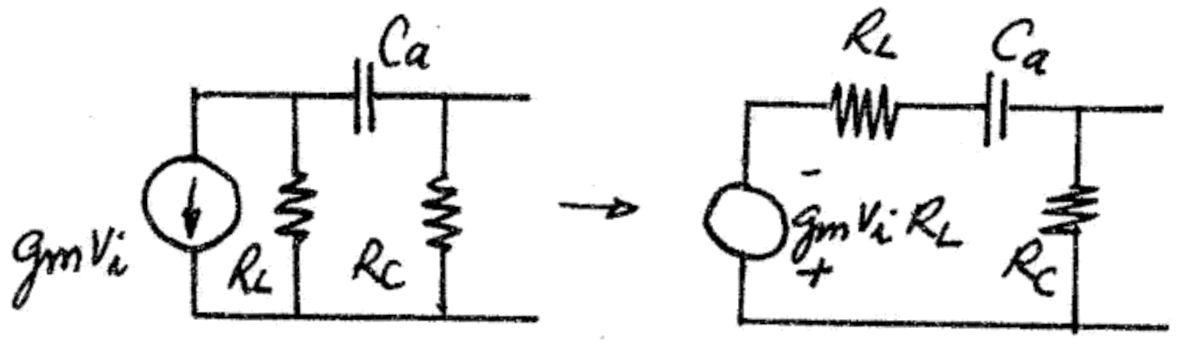
\includegraphics[width=0.6\linewidth]{_fig/respfreq_bjt-eq-thevenin.png}
	\caption{Equivalente de Thevenin}
	\label{fig:respfreq_bjt-eq-thevenin}
\end{figure}

De la Figura \ref{fig:respfreq_bjt-eq-thevenin} tenemos:

\[
V_o' = \left(\frac{-g_m V_i R_L}{R_L + R_C + \frac{1}{sC_a}}\right) R_C
\]

ó

\[
\frac{V_o'}{V_i} = -g_m R_C \parallel R_L \frac{s}{s + \frac{1}{C_a (R_C + R_L)}}
\]

Por lo tanto, dada la relación de \(V_i/V_s\) ya encontrada, tenemos:

\begin{equation} \label{respfreq_bjt-ft-analisis}
	\frac{V_o'}{V_s} = \left(-g_m R_L \parallel R_C \right) \frac{R_B \parallel r_{\pi}}{R_B \parallel r_{\pi} + R_S} \frac{s}{\left(s + \frac{1}{C_i(R_S + R_B \parallel r_{\pi})}\right)\left(s + \frac{1}{C_a(R_C + R_L)}\right)}
\end{equation}

En una comparación entre las funciones dadas en las ecuaciones \ref{respfreq_bjt-ft-analisis} y \ref{respfreq_bjt-ft}, se puede observar que la ganancia a frecuencias medias ha disminuido por el factor: \( \frac{R_L \parallel R_C}{R_L} \) debido al efecto de carga de \(R_C\).

\subsection{Caso del Condensador \( C_a \)}

El condensador \(C_a\) ha creado una pareja de cero y polo; el cero se ubica en el origen, es decir, también impide el paso de corriente continua a la salida. El polo viene dado por:

\[
-\frac{1}{C_a (R_C + R_L)} = -\frac{1}{C_a R_T}
\]

donde \(R_T\) es la resistencia de Thevenin vista desde los bornes de \(C_a\).

En la Figura \ref{fig:respfreq_bjt-bode}, se traza el Diagrama de Bode aproximado de la Ecuación \ref{respfreq_bjt-ft-analisis}, la cual tiene la forma de la Ecuación \ref{respfreq_bodealt-eq}, en donde:

\[
A_M = \frac{\left(-g_m R_L \parallel R_C \right) R_B \parallel r_{\pi}}{R_B \parallel r_{\pi} + R_S}
\]

y 

\[
F_L(s) = s / \left(s + P_{c_i} \right) \left(s + P_{c_a} \right)
\]

donde:

\[
P_{c_i} = \frac{1}{C_i(R_S + R_B \parallel r_{\pi})}
\]

\[
P_{c_a} = \frac{1}{C_a (R_C + R_L)}
\]

Al trazar la curva exacta del módulo de la función de la Ecuación \ref{respfreq_bjt-ft-analisis}, se encontrará que la frecuencia de media potencia es mayor que \( w_{B1} \).

\begin{figure}[h]
	\centering
	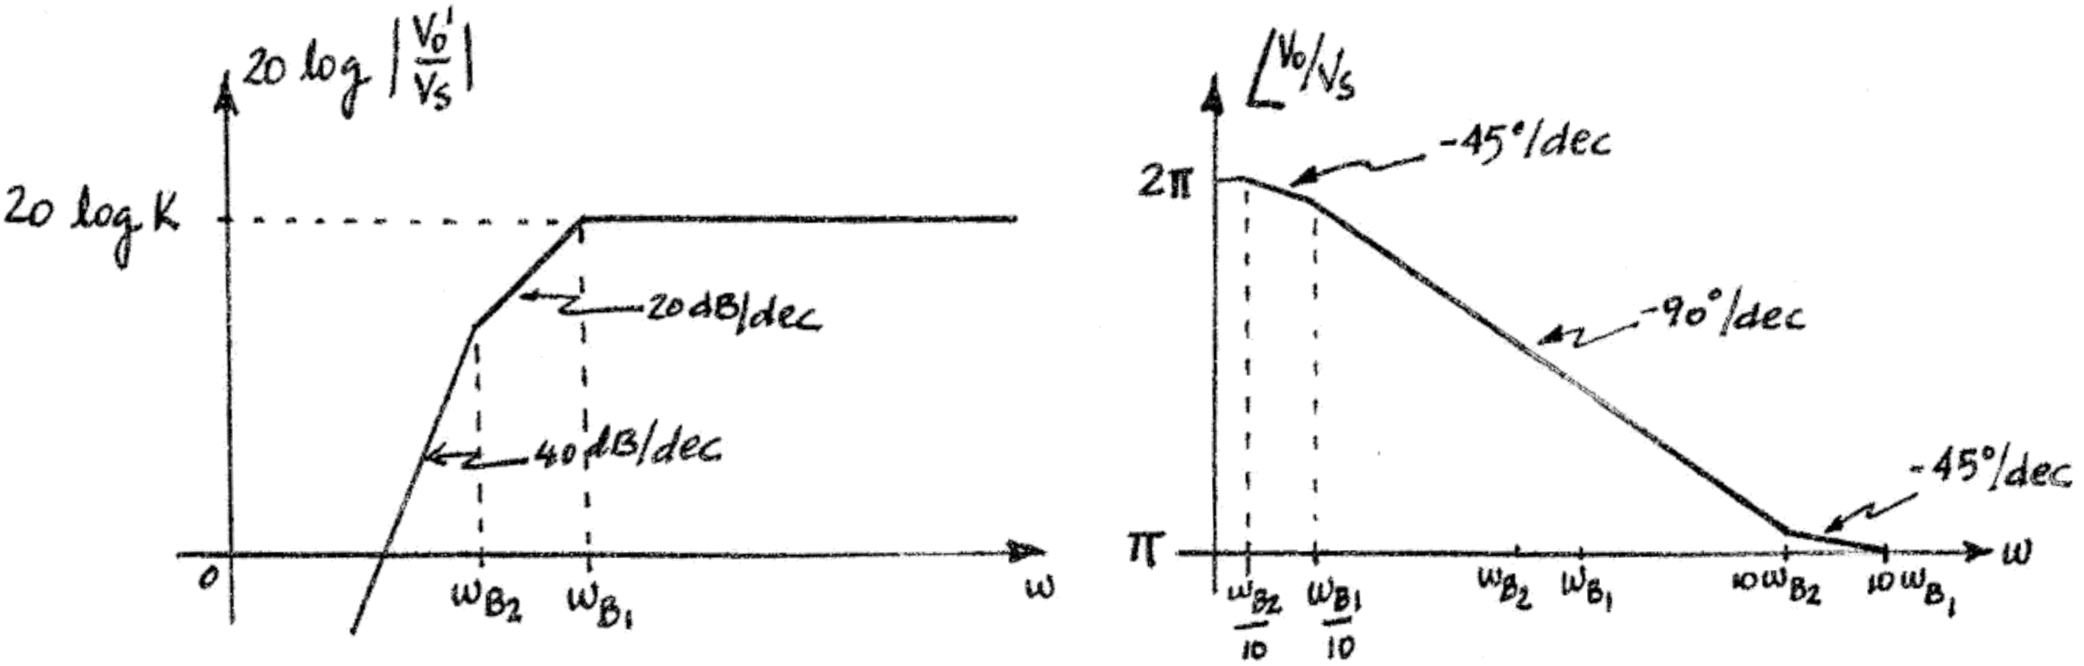
\includegraphics[width=0.9\linewidth]{_fig/respfreq_bjt-bode.png}
	\caption{Diagrama de Bode del circuito de la Fig. 1.32. Aquí se ha supuesto que los polos \( w_{B2} \) y \( w_{B1} \) debido a \( C_i \) y \( C_a \) no son iguales}
	\label{fig:respfreq_bjt-bode}
\end{figure}

\subsection{Caso del Condensador \( C_E \)}

El tercer caso que vamos a tratar es el condensador \( C_E \) que puentea la resistencia del emisor, \( R_E \), de la configuración emisor común, como se muestra en la Figura \ref{fig:respfreq_bjt-ca}, en donde se ha reemplazado la red normal de polarización por \( V_{BB} \) para simplificar el análisis del circuito.

\begin{figure}[h]
	\centering
	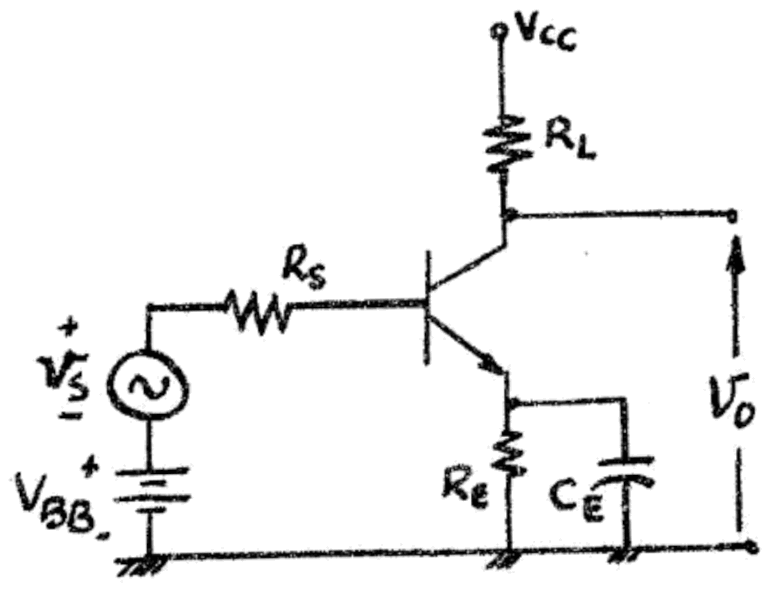
\includegraphics[width=0.5\linewidth]{_fig/respfreq_bjt-ca.png}
	\caption{Circuito BJT en corriente alterna}
	\label{fig:respfreq_bjt-ca}
\end{figure}			

En la Figura \ref{fig:respfreq_bjt-ca2} se ve el mismo circuito para corriente alterna (c.a.), donde el paralelo de \( R_E \) con \( C_E \) se considera una sola impedancia: \( Z_E = R_E \parallel \frac{1}{sC_E} \).

\begin{figure}[h]
	\centering
	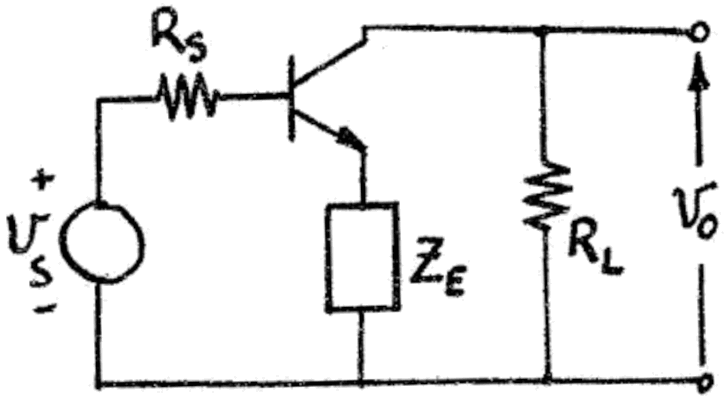
\includegraphics[width=0.5\linewidth]{_fig/respfreq_bjt-ca2.png}
	\caption{Circuito de la Figura \ref{fig:respfreq_bjt-ca} para corriente alterna}
	\label{fig:respfreq_bjt-ca2}
\end{figure}	

Este circuito tiene la misma topología de la configuración en corriente continua (E.C.) con \( R_E \), la única diferencia es que \( R_E \) ha sido reemplazado por \( Z_E \). Por lo tanto, la expresión para la ganancia \( V_o / V_s \) debe ser la misma excepto por esa diferencia.

\begin{equation}
	\frac{V_o}{V_s} = \frac{-\beta R_L}{R_s + r_{\pi} + (\beta+1)Z_E}
\end{equation}

Ahora llevaremos esta función a la forma de la ecuación \ref{respfreq_bodealt-eq}:

\[
\frac{V_o}{V_s} = \frac{-\beta R_L}{R_s + r_{\pi} + \frac{(\beta+1)R_E}{1 + R_E S C_E}}
\]

\[
\frac{V_o}{V_s} = \frac{-\beta R_L (1 + R_{E} S C_E)}{R_s + r_{\pi} + (\beta+1)R_E + R_E S C_E(R_s + r_{\pi})}
\]

\[
\frac{V_o}{V_s} = \frac{-\beta R_L R_{E} C_E (\frac{1}{R_E C_E}+S)}{R_E C_E (R_s + r_{\pi}) [\frac{R_s + r_{\pi} + (\beta+1)R_E}{R_E C_E (R_s + r_{\pi})} + S]}
\]

\begin{equation}\label{respfreq:solve2_vo-vs}
	\frac{V_o}{V_s} = \frac{-\beta R_L}{R_S + r_{\pi})} \frac{(S+\frac{1}{R_E}C_E)}{S+\frac{R_s + r_{\pi}+(\beta+1)R_E}{C_E R_E (R_s + r_{\pi})}}
\end{equation}

El circuito tiene una ganancia a frecuencias medias:

\( \frac{V_o}{V_s} (\omega \to \infty) = \frac{-\beta R_L}{R_s + r_{\pi}} \) exactamente igual a la ganancia de un circuito semejante con el emisor cortocircuitado a tierra.

El circuito tiene un cero, \( Z_1 = \frac{-1}{R_E C_E} \), y un polo, \( p_1 = \frac{R_s + r_{\pi} + (\beta+1)R_E}{C_E R_E (R_s + r_{\pi})} \)

El polo puede ser expresado de otra forma más interesante:

\[
P_1 = \frac{-(\frac{R_s+r_{\pi}}{\beta+1}+R_E)}{C_E R_E (\frac{R_s + r_\pi}{\beta+1})}			
\]

\[
P_1 =  \frac{-1}{C_E R_E \parallel (\frac{R_S+r_{\pi}}{\beta+1})}
\]

Es decir, el polo viene dado por \( -\frac{1}{C_E R_T} \), donde \( R_T \) es la resistencia de Thevenin vista desde los extremos de \(C_E\); \(R_T = R_E \parallel (\frac{R_S+r_{\pi}}{\beta+1}) \).

La expresión para esta resistencia es la misma que para la resistencia de salida de la configuración colector común; esto se debe a que en ambos casos se está viendo la resistencia entre el emisor de un transistor y tierra en paralelo con una \( R_E \) o \( R_L \).

En los tres casos que se han visto hasta ahora, los polos de los condensadores vienen dados por \( \frac{-1}{C R_T} \) donde \( R_T \) es la resistencia de Thevenin vista desde los extremos del condensador. En forma semejante, los ceros vienen dados por \( \frac{1}{C R_H} \), donde $R_H$ es la resistencia directamente en paralelo. Vea el Cuadro \ref{tab:respfreq_polos-ceros} Se hace notar que estas expresiones pueden obtenerse alternativamente por el Método de Superposición.

\begin{table}[h]
	\centering
	\begin{tabular}{|c|c|c|c|}
		\hline
		& $C_i$ & $C_a$ & $C_E$ \\ \hline
		$R_H$ & $\infty$ & $\infty$ & $R_E$ \\ \hline
		cero (z) & 0 & 0 & $\frac{1}{R_E C_E}$ \\ \hline
		$R_{TH}$ & $R_s + R_B \parallel r_{\pi}$ & $R_L + R_C$ & $R_E \parallel \frac{R_s + r_{\pi}}{\beta + 1} $ \\ \hline
		polo(p) & $\frac{-1}{C_i (R_s + R_B \parallel r_{\pi})} )$ & $ \frac{-1}{C_a (R_L + R_C)}$ & $\frac{-1}{C_E R_E \parallel \frac{R_s + r_{\pi}}{\beta+1}}$ \\ \hline
	\end{tabular}
	\caption{Polos y Ceros de los casos \(C_i\), \(C_a\), \(C_E\)}
	\label{tab:respfreq_polos-ceros}
\end{table}

\begin{figure}[h]
	\centering
	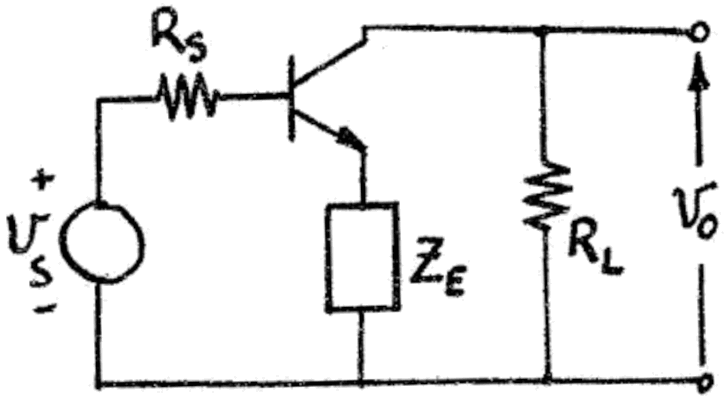
\includegraphics[width=0.5\linewidth]{_fig/respfreq_bjt-ca2.png}
	\caption{Circuito de la Figura \ref{fig:respfreq_bjt-ca} para corriente alterna}
	\label{fig:respfreq_solve2_bode}
\end{figure}	

Se traza el Diagrama de Bode aproximado de la ecuación \ref{respfreq:solve2_vo-vs} en la Figura \ref{fig:respfreq_bode_bjt_ca}. Se hace notar que necesariamente el valor del cero es menor que el valor del polo ya que:

\[
R_E > R_E \parallel \frac{R_s + r_{\pi}}{\beta + 1}
\]

\begin{figure}[h]
	\centering
	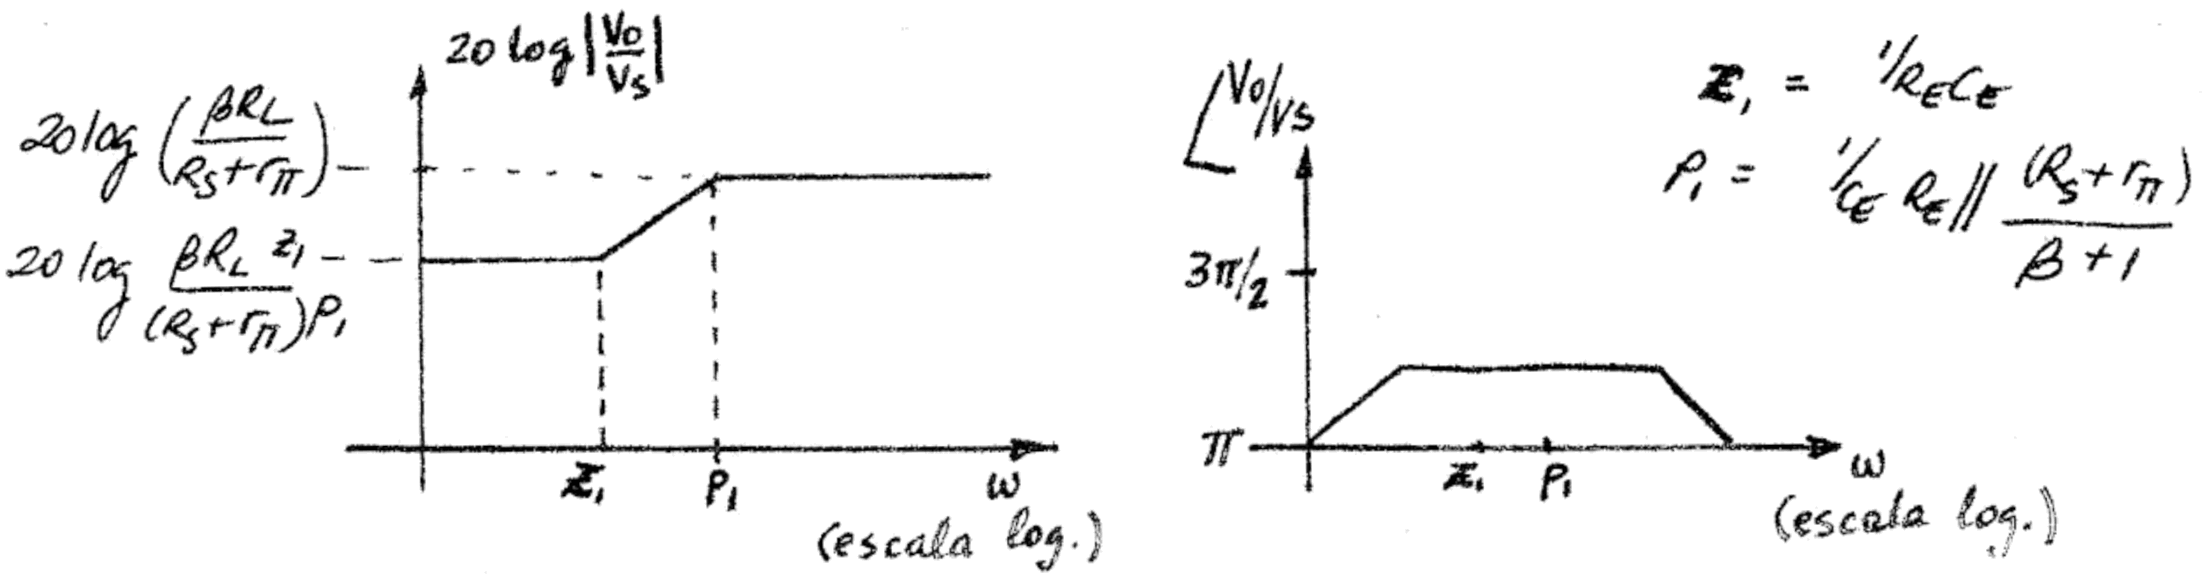
\includegraphics[width=0.8\linewidth]{_fig/respfreq_bode_bjt_ca.png}
	\caption{Diagrama de Bode de la Figura \ref{fig:respfreq_bjt-ca}}
	\label{fig:respfreq_bode_bjt_ca}
\end{figure}

El valor de la ganancia para \( \omega << z_1 \), es:

\begin{equation}
	\frac{V_o}{V_s} = \frac{-\beta R_L z_1}{(R_s + r_{\pi}) p_1} = \frac{-\beta R_L}{R_s + r_{\pi} + (\beta+1)R_E}
\end{equation}

A la vez, esta expresión la reconocemos como la ganancia de la configuración emisor común con \( R_E \); esto es lógico ya que a frecuencias suficientemente bajas, el condensador se comporta como un circuito abierto, y el circuito de la figura 1.37 queda como un E.C. con \( R_E \).

\begin{figure}[h]
	\centering
	\subfloat[Circuito Original]
	{
		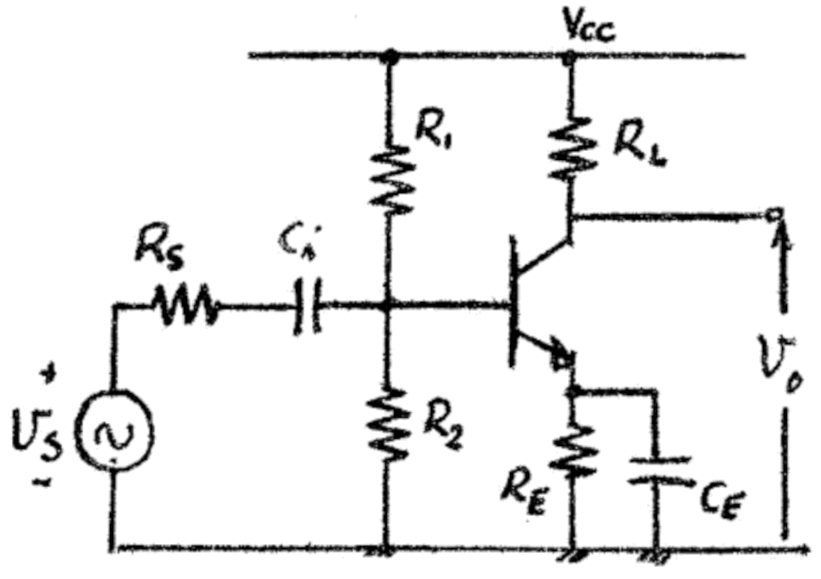
\includegraphics[width=0.44\linewidth]{_fig/respfreq_emisor-comun-autolarizado_original.png}
		\label{fig:respfreq_emisor-comun-autolarizado_original}
	}
	\subfloat[Equivalente para C.A.]
	{
		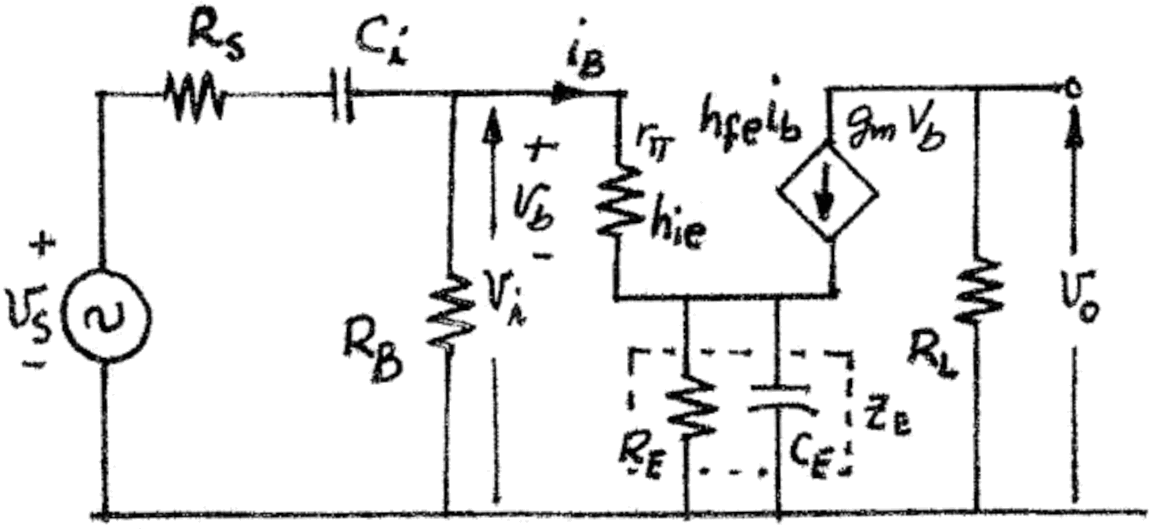
\includegraphics[width=0.44\linewidth]{_fig/respfreq_emisor-comun-a_equiv-ca.png}
		\label{fig:respfreq_emisor-comun-a_equiv-ca}
	}
	\caption{Emisor Común Autopolarizado}
	\label{fig:respfreq_emisor-comun-autolarizado}
\end{figure}

\subsubsection{Ejemplo 4} \label{respfreq_ejm4}

Determine la función de transferencia del circuito de la Figura \ref{fig:respfreq_emisor-comun-autolarizado} por el Método Exacto y el Método de Superposición.

\textbf{Solución:}

Para hallar la función de transferencia exacta, \( \frac{V_o}{V_s}(s) \), se trabaja con las ecuaciones de malla y nodo de este circuito. Así:

\[
v_o =  - \beta i_B R_L
\]

\[
i_B = \frac{V_i}{Z_i}
\]

donde \( Z_i = r_{\pi} + (\beta + 1)Z_E \), donde \( Z_E = \frac{R_E}{(1 + {s R_E C_E}} \)

y,

\[
v_i = \frac{{R_B \parallel Z_i}V_S}{{R_B \parallel  Z_i} + \frac{1}{S C_i} + R_s} = \frac{R_B Z_i S C_i V_s}{{R_B Z_i S C_i}+(R_B + Z_i)(1+ {S C_i R_s})}
\]

Uno ahora reemplaza $Z_i$ por su expresión equivalente y se trabaja con las expresiones hasta conseguir \( V_o/V_s \) de la forma:

\[
\frac{V_o}{V_s} = K \frac{s(s+\omega_1)}{s^2+bs+c}
\]

Sin embargo, al hacerlo, uno se convence rápidamente que es una labor muy engorrosa, resultando una cantidad de productos y sumas que difícilmente pueden interpretarse en relación al circuito, y además se presta para equivocaciones. ¡Como sería con 3 condensadores!

\textbf{Por el Método de Superposición:}

\begin{figure}[h]
	\centering
	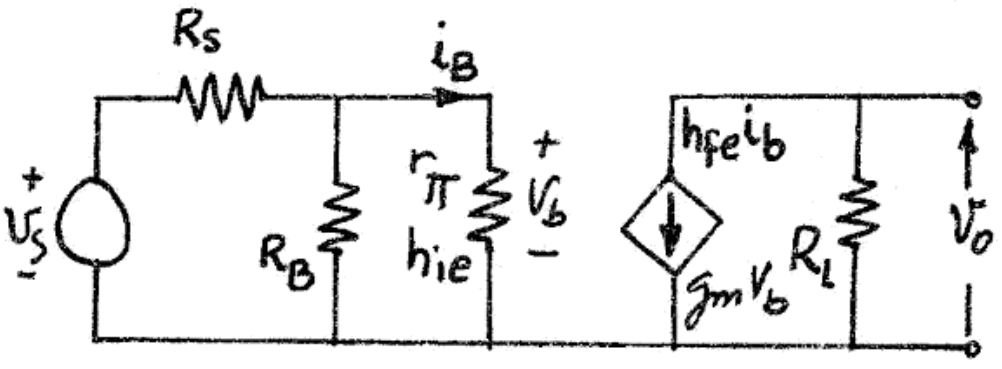
\includegraphics[width=0.8\linewidth]{_fig/respfreq_emisor-comun-autolarizado_c-short.png}
	\caption{Figura \ref{fig:respfreq_emisor-comun-autolarizado} con los C's cortocircuitados}
	\label{fig:respfreq_emisor-comun-autolarizado_c-short}
\end{figure}

\textbf{a)} El circuito a frecuencias medias, \( \omega_m \), para calcular \( A_M \) se muestra en la \ref{fig:respfreq_emisor-comun-autolarizado_c-short}, de donde se consigue:

\[
\frac{V_o}{V_s}(\omega_m) = A_M = \frac{-g_m R_L {R_{B} \parallel r_{\pi}}}{(R_s + {R_{B} \parallel r_{\pi}}}
\]

\begin{figure}[h]
	\centering
	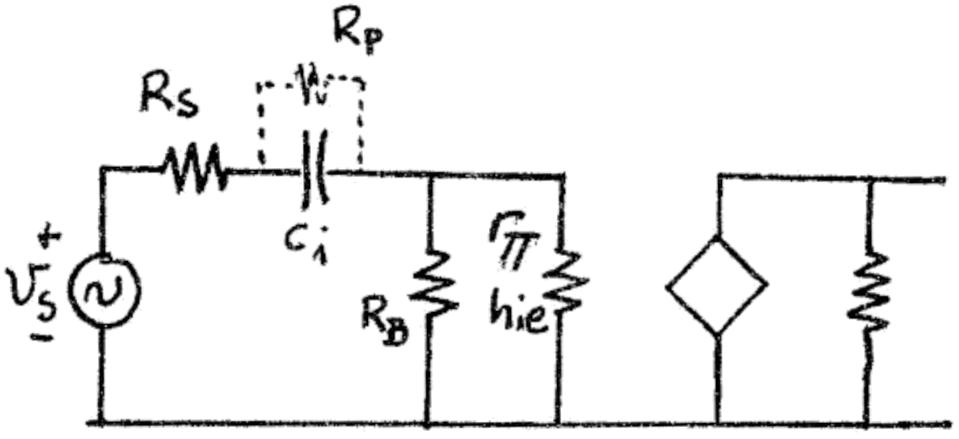
\includegraphics[width=0.8\linewidth]{_fig/respfreq_emisor-comun-autolarizado_calc_ci.png}
	\caption{Circuito apto para calcular \( \frac{s+z_{ci}}{s+p_{ci}} \)}
	\label{fig:respfreq_emisor-comun-autolarizado_calc_ci}
\end{figure}

\textbf{b)} El circuito para calcular polo y cero debido a $C_i$ se muestra en la Figura \ref{fig:respfreq_emisor-comun-autolarizado_calc_ci}.

La $R_p$ en paralelo con $C_i = \infty$.

La $R_T$ vista desde $C_i = R_s + R_{B} \parallel r_{\pi}$.

\begin{figure}[h]
	\centering
	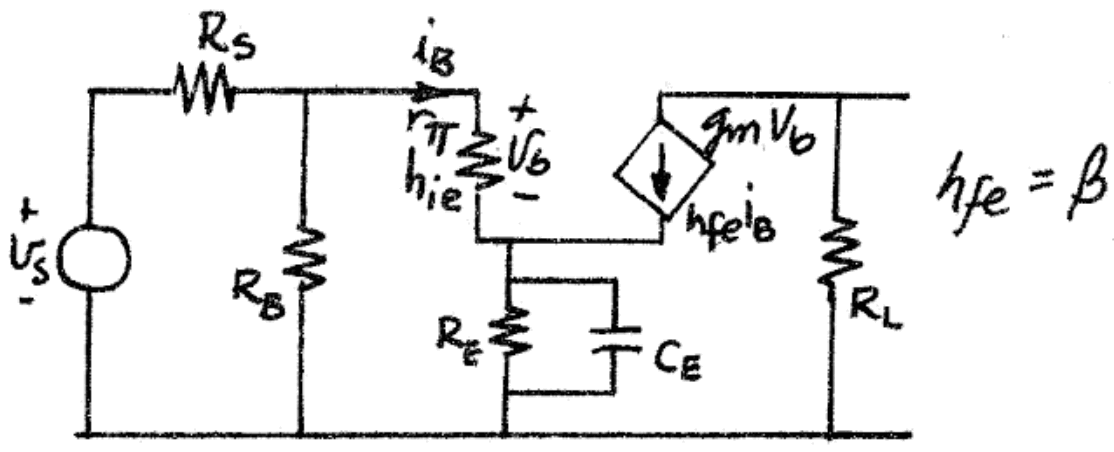
\includegraphics[width=0.8\linewidth]{_fig/respfreq_emisor-comun-autolarizado_calc_ce.png}
	\caption{Circuito apto para los polos y ceros debido a $C_E$}
	\label{fig:respfreq_emisor-comun-autolarizado_calc_ce}
\end{figure}

\textbf{c)} El circuito para calcular polo y cero debido a $C_E$ se muestra en la Figura \ref{fig:respfreq_emisor-comun-autolarizado_calc_ce}.

La $R_p = R_E$.

La $R_T = R_E \parallel \frac{R_s + R_{B} + r_{\pi}}{\beta + 1} $

\textbf{d)} En total, la función de transferencia queda:

\begin{equation}
	\frac{V_o}{V_s}(s) = \frac{-g_m R_L R_{B} \parallel r_{\pi}}{R_{B} \parallel r_{\pi} + R_s} \frac{s {s + \frac{1}{R_E C_E}}}{(s + \frac{1}{C_i (R_s + R_{B} \parallel r_{\pi})})(s + \frac{1}{C_E (R_E \parallel \frac{R_s + r_{\pi}}{\beta + 1})})}
\end{equation}

\section{Un modelo de transistor apto para altas frecuencias} %p44

Los amplificadores transistorizados, como el de la Figura \ref{fig:respfreq_bjt-base}, sufren pérdidas en su ganancia a frecuencias altas que no se preveen de acuerdo al modelo simplificado híbrido. Surge la necesidad de algo más para el estudio a altas frecuencias.

Existen dos mecanismos en el transistor cuyo efecto es capacitivo:

\begin{enumerate}
	\item Una capacitancia de difusión para la junta directamente polarizada, dependiente del nivel de corriente contínua del colector, $I_C$
	\item Dos capacitancias, una a través de cada junta, que son dependientes de la tensión a través de esas juntas, como se indica en la Figura \ref{fig:respfreq_transistor-cap-internas}.
\end{enumerate}

\begin{figure}[h]
	\centering
	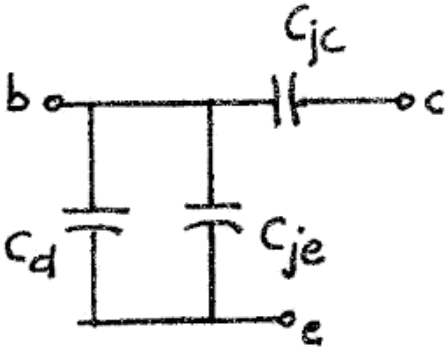
\includegraphics[width=0.5\linewidth]{_fig/respfreq_transistor-cap-internas.png}
	\caption{Capacitancias internas del transistor}
	\label{fig:respfreq_transistor-cap-internas}
\end{figure}

Hay caídas de Voltaje en la base entre los bornes externos y la región interna de operación, tal como se indica en la Figura \ref{fig:respfreq_transistor-construccion-y-regiones}. Esta se representa en el modelo por $r_b$.

\begin{figure}[h]
	\centering
	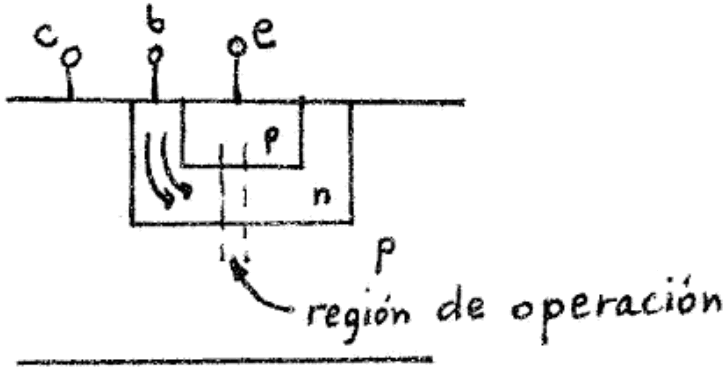
\includegraphics[width=0.5\linewidth]{_fig/respfreq_transistor-construccion-y-regiones.png}
	\caption{Construcción Física del Transistor y la Región de Operación}
	\label{fig:respfreq_transistor-construccion-y-regiones}
\end{figure}		

Se anexan las capacitancias de junta y de difusión, la resistencia $r_b$ al modelo $\pi$ híbrido simplificado para llegar al modelo $\pi$ híbrido de alta frecuencia que se muestra en la Figura \ref{fig:respfreq_transistor-modelo-hf}.

\begin{figure}[h]
	\centering
	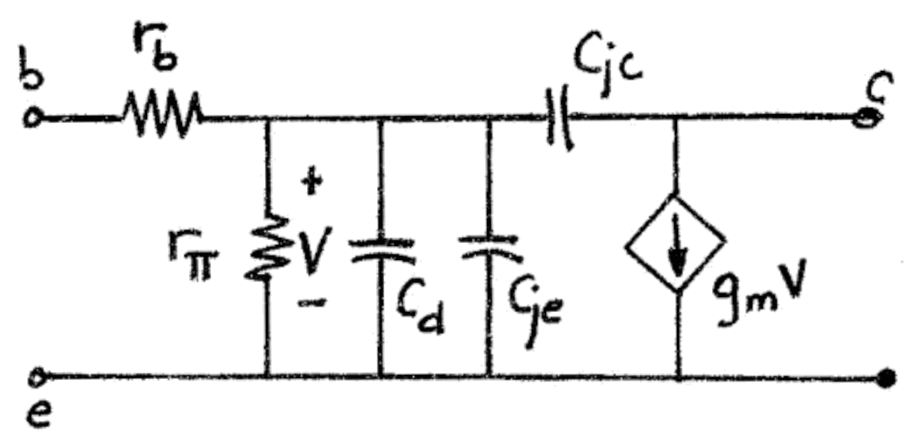
\includegraphics[width=0.6\linewidth]{_fig/respfreq_transistor-modelo-hf.png}
	\caption{Modelo híbrido de alta frecuencia}
	\label{fig:respfreq_transistor-modelo-hf}
\end{figure}

Una variación de tensión en la unión colector base produce una ligera modificación del ancho de la base, que a su vez produce un cambio en la corriente de colector. Este efecto se representa con una conductancia $g_{bc}$ entre el colector y la base interna, $b'$. Para completar el modelo se anexa una conductividad, $g_{ce}$, entre el colector y el emisor. El modelo completo se muestra en la Figura \ref{fig:respfreq_transistor-hibrido-completo}.

\begin{figure}[h]
	\centering
	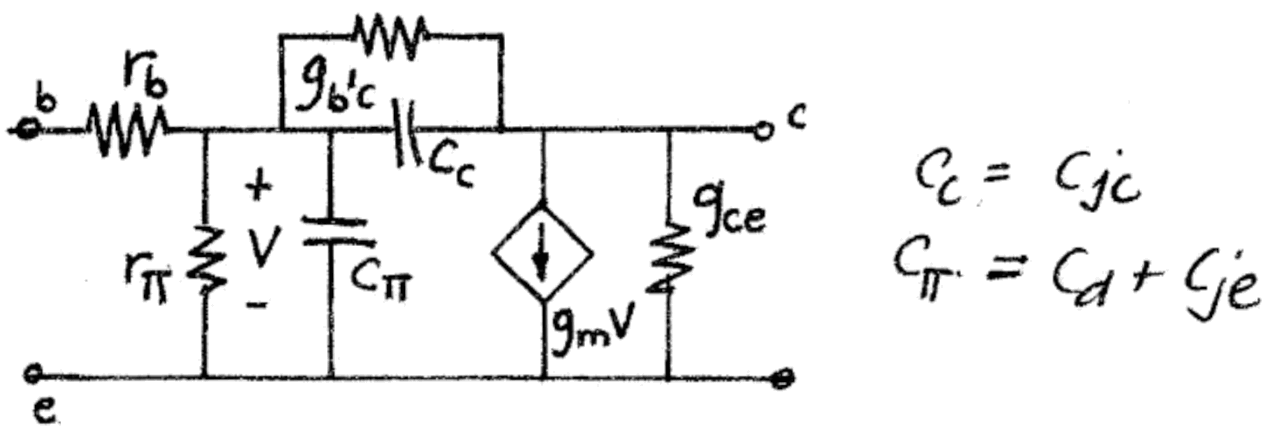
\includegraphics[width=0.5\linewidth]{_fig/respfreq_transistor-hibrido-completo.png}
	\caption{Modelo híbrido completo}
	\label{fig:respfreq_transistor-hibrido-completo}
\end{figure}

$C_c = C_{jc}$

$C_{\pi} = C_d + C_{je}$

\subsection{Comparación con el Modelo de los Parámetros $h$}

Relacionamos el modelo $\pi$ híbrido a bajas frecuencias, donde las capacitancias se desprecian en la forma de un circuito abierto, con un modelo muy conocido, el de los parámetros h, tal como se ven en la Figura \ref{fig:respfreq_model-t}.

\begin{figure}[h]
	\centering
	\subfloat[Modelo $\pi$ híbrido a bajas frecuencias]
	{
		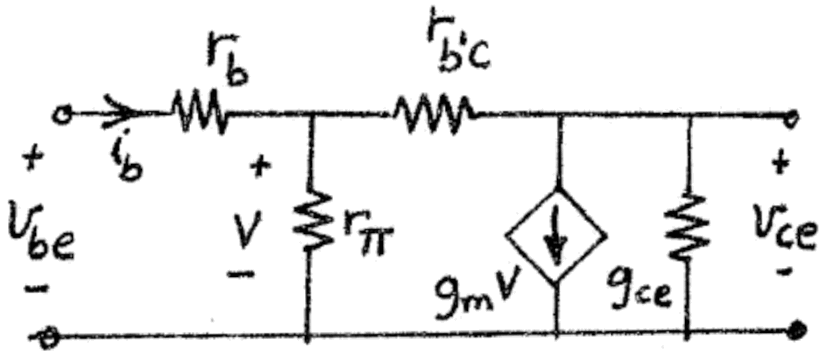
\includegraphics[width=0.44\linewidth]{_fig/respfreq_model-t_pi-hibrido.png}
		\label{fig:respfreq_model-t_pi-hibrido}
	}
	\subfloat[Modelos de los paránmetros $h$]
	{
		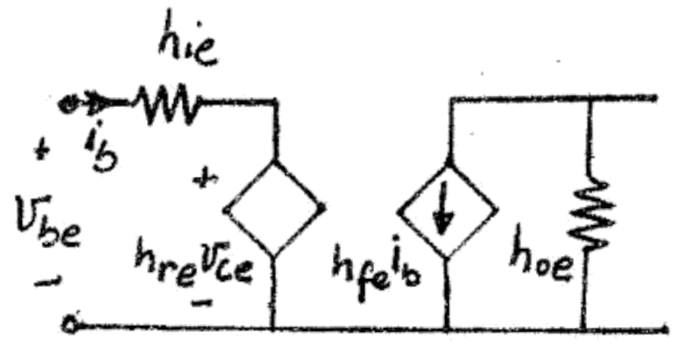
\includegraphics[width=0.44\linewidth]{_fig/respfreq_model-t_parametros-h.png}
		\label{fig:respfreq_model-t_parametros-h}
	}
	\caption{Modelos del transistor}
	\label{fig:respfreq_model-t}
\end{figure}

\begin{enumerate}
	\item La corriente de salida del circuito con la salida en corto circuito es $g_m v$ en un caso y $h_{fe} i_b$ en el otro. $h_{fe}$ es la ganancia de corriente en ortocircuito y es igual a $\beta$ del transistor.
	
	Entonces, $g_m v = h_{fe} i_b$ si suponemos que $r_{bc} \approx \infty$ da $v = i_b r_{\pi}$ y $g_m i_b r_{\pi} = h_{fe} i_b$ ó:
	
	\begin{equation}
		g_m r_{\pi} = h_{fe}
	\end{equation}
	
	\item Con la entrada abierta, $h_{re} = \frac{v}{v_{ce}}$ es la ganancia inversa de voltaje. A la vez:
	
	\begin{equation}
		\frac{v}{v_{ce}} = \frac{r_{\pi}}{r_{\pi} + r_{bc}} \to r_{bc} = \frac{r_{\pi}}{h_{re}}
	\end{equation}
	
	que se ve es un valor muy grande pues $h_{re}$ es siempre muy pequeño.
	
	\item La impedancia de entrada con la salida en cortocircuito es:
	
	\begin{equation}
		h_{ie} = r_{\pi} + r_b
	\end{equation}
	
	\item Con la entrada en circuito abierto se consigue $h_{oe}$, la admitancia de salida:
	
	\[
	i_c = v_{ce} g_{ce} + \frac{v_{ce}}{r_{bc} + r_{\pi}} + g_m V = v_{ce} \left[ g_{ce} + \frac{1}{r_{bc} + r_{\pi}} + \frac{g_m r_{\pi}}{r_{bc} + r_{\pi}} \right]
	\]
	
	de donde
	
	\[
	h_{oe} = \frac{i_c}{v_{ce}} = g_{ce} + \frac{h_{re} + 1}{r_{bc} + r_{\pi}}
	\]
	
	ó
	
	\begin{equation}
		g_{ce} = h_{oe} - \frac{(h_{re} + 1)}{r_{bc} + r_{\pi}}
	\end{equation}
	
\end{enumerate}

Generalmente despreciamos $h_{oe}$ y $h_{re}$ en el modelo de los parámetros $h$ y se desprecia $g_{ce}$ y $g_{bc}$ en el modelo $\pi$ híbrido. El modelo simplificado se ve en la Figura \ref{fig:respfreq_transistor-hibrido-simplificado}. Se hace notar que se puede utilizar este modelo para bajas frecuencias eliminando los condensadores.

\begin{figure}[h]
	\centering
	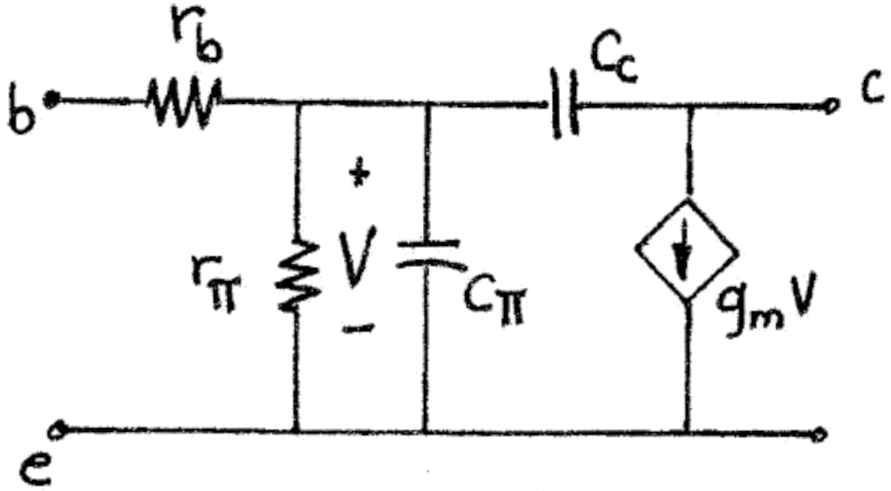
\includegraphics[width=0.5\linewidth]{_fig/respfreq_transistor-hibrido-simplificado.png}
	\caption{Modelo $\pi$ híbrido Simplificado}
	\label{fig:respfreq_transistor-hibrido-simplificado}
\end{figure}

Se ha relacionado los elementos del modelo $\pi$ híbrido a frecuencias bajas con los del modelo de los parámetros $h$; en caso que el fabricante de un transistor suministra valores de los parámetros $h$, de ellos se puede calcular los valores de los parámetros $g_m$, $r_{\pi}$ y $r_b$ del modelo simplificado.

\begin{figure}[h]
	\centering
	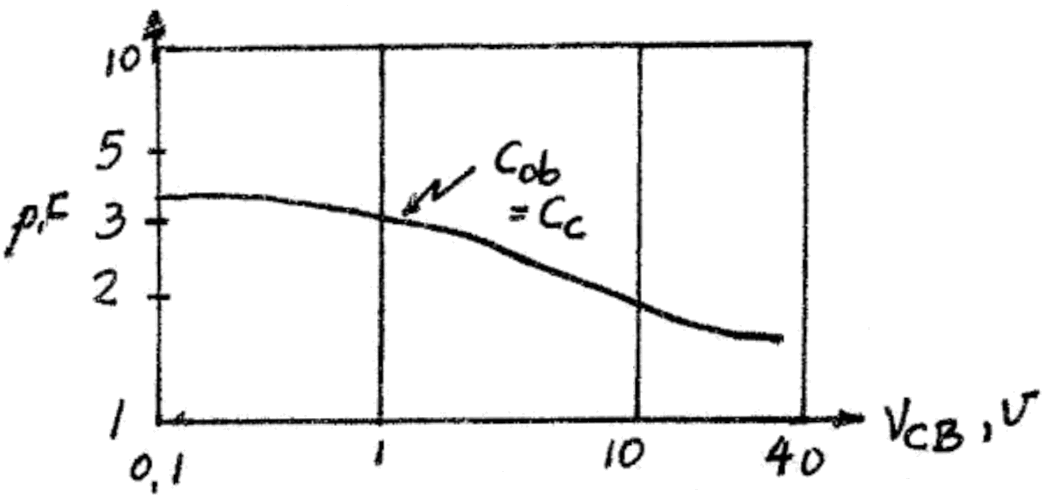
\includegraphics[width=0.5\linewidth]{_fig/respfreq_transistor-cap-junta-cb.png}
	\caption{Capacitancia de junta en función del voltaje $V_{CB}$}
	\label{fig:respfreq_transistor-cap-junta-cb}
\end{figure}

El valor de $C_c$ es inversamente proporcional al voltaje colector base. El fabricante generalmente especifica esta relación por medio de una gráfica entre las hojas de datos del transistor. Por ejemplo para el 2N3904 de Motorola aparece la gráfica de la Figura \ref{fig:respfreq_transistor-cap-junta-cb} para $C_{ob} = C_c$. Una ecuación que describe adecuadamente esta gráfica es:

\begin{equation}
	C_c \approx \frac{C_o}{(1 + V_{CB}/V_j)^{1/2}}
\end{equation}

donde $C_o$ es el valor de $C_c$ para $V_{CB} = 0$.

El valor de $c_\pi$ es función de $f_T$, donde $f_T$ es el producto ganancia ancho de banda de corriente para un transistor y su valor viene dado por el fabricante. $\omega_p$ se define como la frecuencia a la cual la ganancia de corriente baja a $1/\sqrt{2}$ de su valor máximo, con la salida en corto circuito; como se ve en la Figura \ref{fig:respfreq_transistor-salida-cortocircuito}. Se obtiene la corriente de salida, $I_o = -g_m v$. La transconductancia, $g_m$, no es función de la frecuencia; en cambio $v$ sí lo es.

\begin{figure}[h]
	\centering
	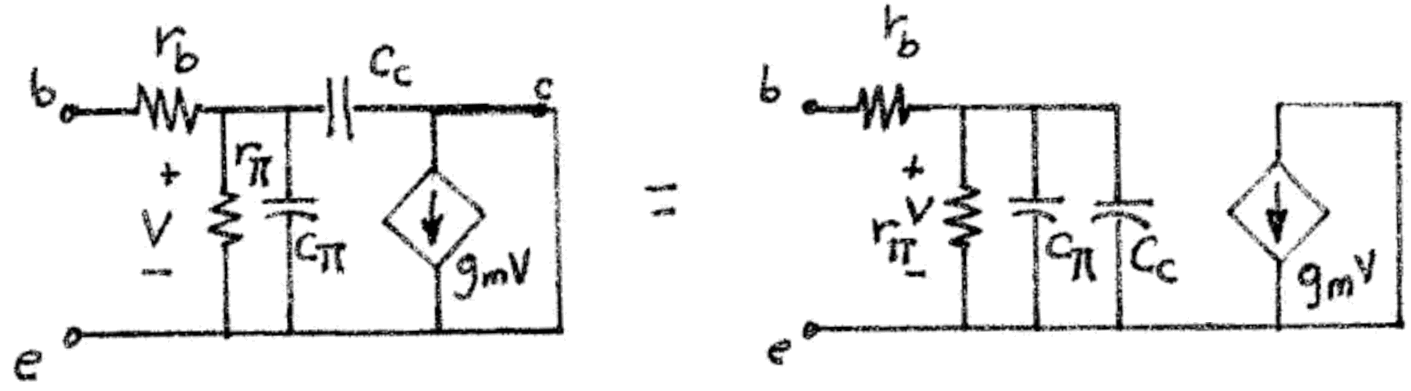
\includegraphics[width=0.8\linewidth]{_fig/respfreq_transistor-salida-cortocircuito.png}
	\caption{Modelo del Transistor con la Salida en Cortocircuito}
	\label{fig:respfreq_transistor-salida-cortocircuito}
\end{figure}

Se tiene que:

\[
I_i = v(g_{\pi} + s(C_{\pi} + C_c))
\]

\begin{equation}
	\frac{V}{I_i} = \frac{1}{(g_{\pi} + s(C_{\pi} + C_c))}
\end{equation}

e

\begin{equation}
	\frac{I_o}{I_i}(s) = \frac{-g_m V}{I_i} = \frac{-g_m}{g_{\pi} + s(C_{\pi} + C_c)}
\end{equation}

Esta función se grafica en la Figura \ref{fig:respfreq_transistor-corriente-funcion-omega}. La frecuencia de corte es:

\begin{equation} \label{respfreq_transistor_freq-corte}
	\omega_B = \frac{g_{\pi}}{C_{\pi} + C_c}
\end{equation}

\begin{figure}[h]
	\centering
	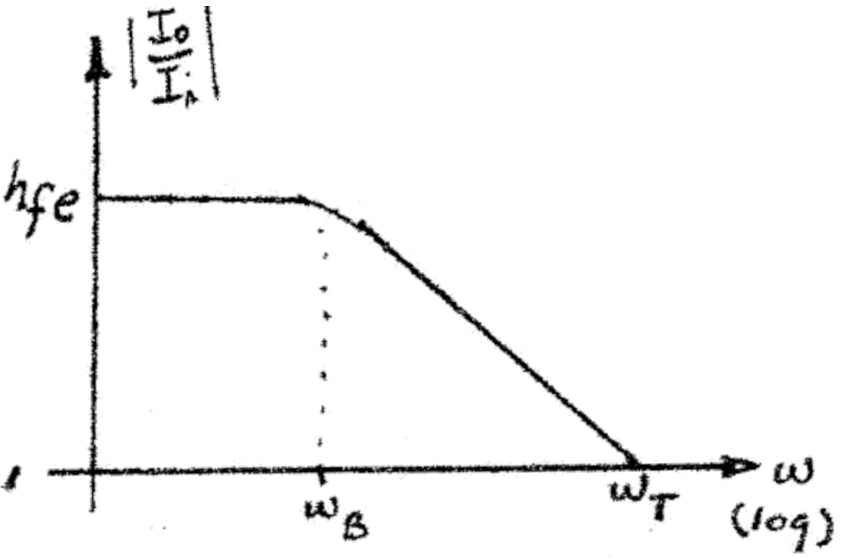
\includegraphics[width=0.8\linewidth]{_fig/respfreq_transistor-corriente-funcion-omega.png}
	\caption{Ganancia de Corriente en función de $\omega$}
	\label{fig:respfreq_transistor-corriente-funcion-omega}
\end{figure}

y entonces:

\[
\frac{I_o}{I_i}(s) = \frac{-g_m r_{\pi}}{1 + { S r_{\pi}  (C_{\pi} + C_C)} } = \frac{-\beta}{1 + s/\omega_B}
\]

A la frecuencia $\omega_T$ la ganancia baja por definición al valor de uno. A continuación se demuestra que esto ocurre para

\begin{equation} \label{respfreq_transistor_omega-t}
	\omega_T = \beta \omega_B \quad (1.61)
\end{equation}

pues entonces:

\[
\left| \frac{I_o}{I_i}(\omega_T) \right| = \frac{|-\beta|}{|1 + j \beta \omega_B / \omega_T|} \approx 1
\]

de la ecuación \ref{respfreq_transistor_omega-t} se entiende por que se conoce como el producto ganancia ancho de banda. De las ecuaciones \ref{respfreq_transistor_freq-corte} y \ref{respfreq_transistor_omega-t}, se tiene:

\begin{equation} \label{respfreq_transistor-pi-hibrido}
	\omega_T = \frac{\beta}{(C_{\pi} + C_c) r_{\pi}} = \frac{g_m}{C_{\pi} + C_c}
\end{equation}

de donde:

\begin{equation}
	C_{\pi} = \frac{g_m}{\omega_T} - C_c
\end{equation}

Se hace notar que en vista de que $g_m$ es función de $I_c$, el valor de $C_{\pi}$ es también función de $I_c$; aumenta con $I_c$.

En la Tabla \ref{tab:respfreq_modelo-hibrido} se resumen las ecuaciones utilizadas en la obtención de los valores de los elementos del modelo híbrido. La ecuación para $r_b$ carece de precisión al representar la pequeña diferencia entre dos valores grandes, y se establecen los siguientes límites.

\begin{equation}
	50 < r_b < 250
\end{equation}

de acuerdo a la gráfica que relaciona $r_b$ con $I_c$, la Figura \ref{fig:respfreq_transistor_rb-vs-ic}.

\begin{table}[h]
	\centering
	\begin{tabular}{|c|c|}
		\hline
		PARAMETRO & RELACION \\ \hline
		$g_m$ & $I_c q / V_T$ \\ \hline
		$r_{\pi}$ & $h_{fe} / g_m$ \\ \hline
		$r_b$ & $h_{ie} - r_{\pi}$ \\ \hline
		$C_c (V_{CB})$ & $C_o / (1+V_{CB}/V_j)^{1/2}$ \\ \hline
		$C_{\pi}$ & $g_m / \omega_T - C_c$ \\ \hline
	\end{tabular}
	\caption{Parámetros Modelo híbrido}
	\label{tab:respfreq_modelo-hibrido}
\end{table}

\begin{figure}[h]
	\centering
	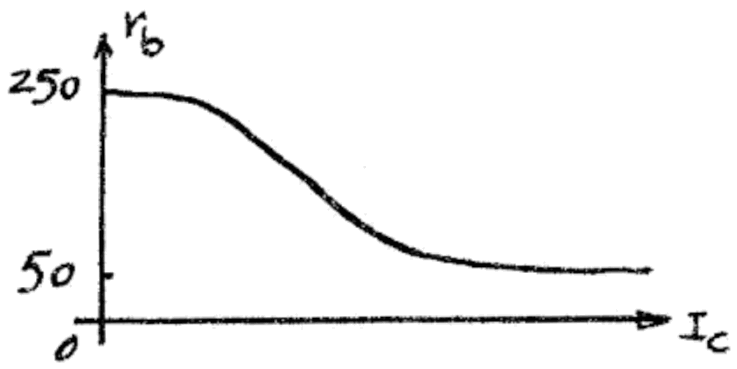
\includegraphics[width=0.8\linewidth]{_fig/respfreq_transistor_rb-vs-ic.png}
	\caption{$r_b$ vs $I_c$}
	\label{fig:respfreq_transistor_rb-vs-ic}
\end{figure}

\subsubsection{Ejemplo 5} \label{respfreq_ejm5}

Hallar los valores de los elementos del modelo híbrido para el circuito de la Figura \ref{fig:respfreq_ejemplo_t-ec_autopolarizado}; utilice $h_{fe} = 180$.

\begin{figure}[h]
	\centering
	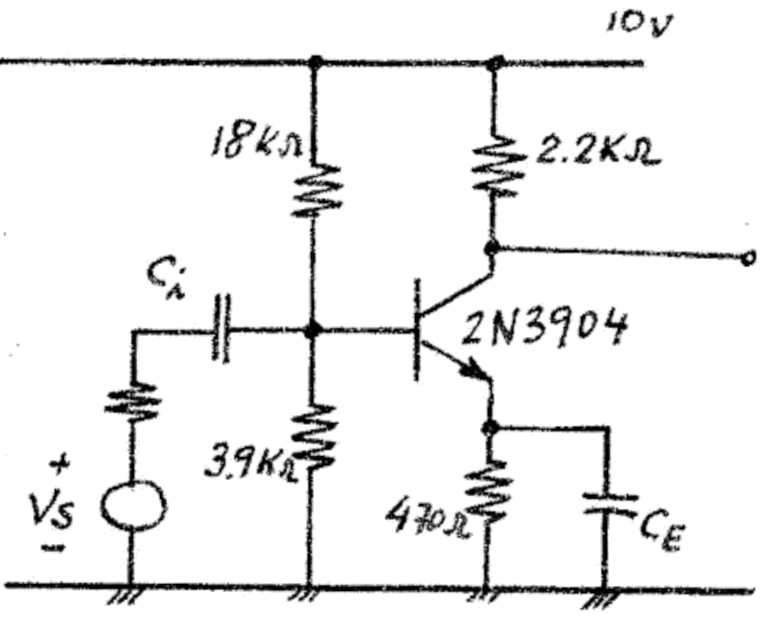
\includegraphics[width=0.8\linewidth]{_fig/respfreq_ejemplo_t-ec_autopolarizado.png}
	\caption{Amplificador EC autopolarizado}
	\label{fig:respfreq_ejemplo_t-ec_autopolarizado}
\end{figure}

\textbf{Solución:}

\textbf{a)} Hallar $V_{CE}$ e $I_C$

Sacando el equivalente de Thevenin en continua en la base nos da:

\[
1.78V = I_B \times 32K + 0.6V + (181) I_B \times 470
\]

ó $I_B = 23.3 \mu A$ e $I_C = 2.33 mA$

Con las hojas de datos del 2N3904 y el valor $I_C = 2.3 mA$, encontramos los valores de $h_{fe} = 150$ y $h_{ie} = 1800$.

Entonces:

\[
g_m = \frac{I_C}{V_T} = \frac{2.33 mA}{26 mV} = 0.0896 mho
\]

\[
r_{\pi} = \frac{\beta}{g_m} = \frac{150}{0.0896} = 1670 \Omega
\]

\[
r_b = h_{ie} - r_{\pi} = 130 \quad \text{(está dentro de los límites)}
\]

Después para $C_c$ hallamos primero $V_{CB} = V_{CE} - V_{BE}$

donde \( V_{CE} = V_{CC} - I_C R_L - I_E R_E \)

\[ V_{CE} = 10 - 2.33 (2.2 + 0.47) = 3.78 V \]

es decir \( V_{CB} = 3.18 V \) y \( C_C (3.18 V) \approx 2 pF \)

Luego:

\( C_{\pi} = \frac{g_m}{\omega_T} - C_c \), \(\omega_T = 2 \pi f_T\) y \(f_T = 300 MHz\) para el 2N3904; por lo tanto \( C_{\pi} = \frac{0.896}{2 \pi 3 \times 10^8} - 2 \times 10^{-12} = 45.5 pF \)

El circuito de la Figura \ref{fig:respfreq_ejemplo_t-ec_autopolarizado} queda con el modelo de la Figura \ref{fig:respfreq_ejemplo_t-ec_ac} para corriente alterna.

\begin{figure}[h]
	\centering
	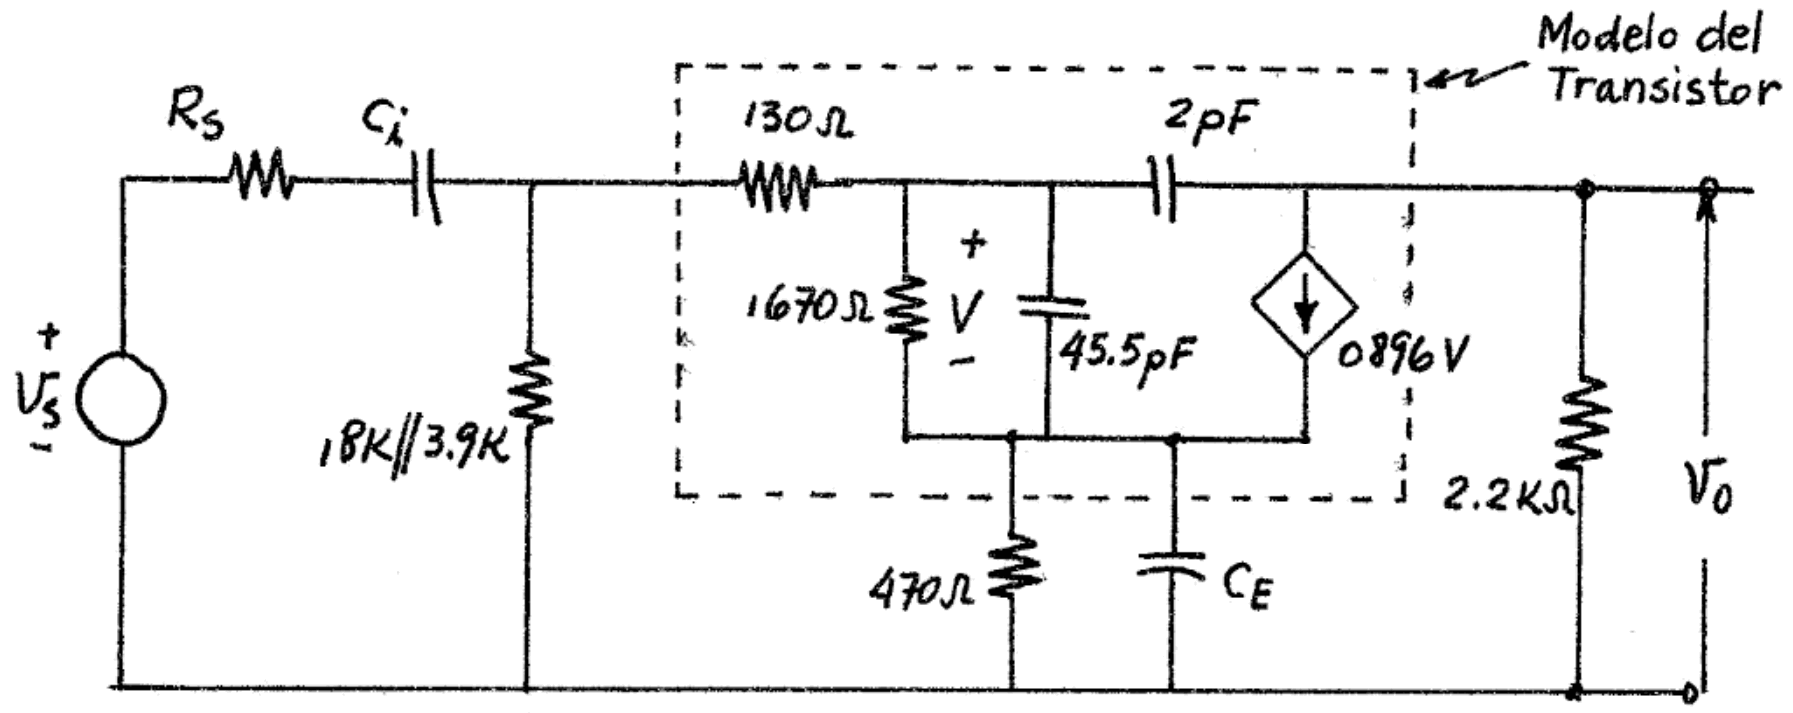
\includegraphics[width=0.8\linewidth]{_fig/respfreq_ejemplo_t-ec_ac.png}
	\caption{El circuito de la Figura \ref{fig:respfreq_ejemplo_t-ec_autopolarizado} para C.A.}
	\label{fig:respfreq_ejemplo_t-ec_ac}
\end{figure}

Se tiene un modelo de alta frecuencia, y se aplica una configuración emisor común para determinar la respuesta de frecuencia para altas frecuencias, como se indica en la Figura \ref{fig:respfreq_emisor-comun-autolarizado_c-short}.

Se quiere la función de transferencia \( V_O / V_S (s) \). Se hace la observación que en el circuito \( (c) \) a analizar, hay menos nodos que mallas, y por lo tanto es más rápido el análisis por ecuaciones de nodo que por ecuaciones de malla. Se tiene 3 nodos: \( b' \), \( c \), y tierra, por lo que se tiene que plantear dos ecuaciones de nodo:

en \( b' \):

\[ V (g_{\pi} + S C_{\pi}) + (V - V_S) g_b' + (V - V_o) S C = 0 \]

en c:

\begin{equation}			
	(V_o - V) s C_c + g_m V + V_o G_L = 0
\end{equation}

Separando los coeficientes de las incógnitas:

\begin{equation}			
	V (g_{\pi} + s C_{\pi} + g_b') + (-s C_c) + V_o (-s C_c) = g_b' V_S'
\end{equation}
\begin{equation}			
	V (g_m - s C_c) + V_o (s C_c + G_L) = 0
\end{equation}

Se puede utilizar la regla de Cramer para despejar \( V_o \):

\begin{equation}
	V_o = \frac{
		\begin{vmatrix}
			g_{\pi} + s C_{\pi} + g_b' + s C_c & g_b' V_S' \\
			g_m - s C_c & 0
		\end{vmatrix}
	}{
		\begin{vmatrix}
			g_{\pi} + s C_{\pi} + g_b' + s C_c & -s C_c \\
			g_m - s C_c & s C_c + G_L
		\end{vmatrix}
	}
\end{equation}

\begin{figure}[h]
	\centering
	\subfloat[Configuración E.C.]
	{
		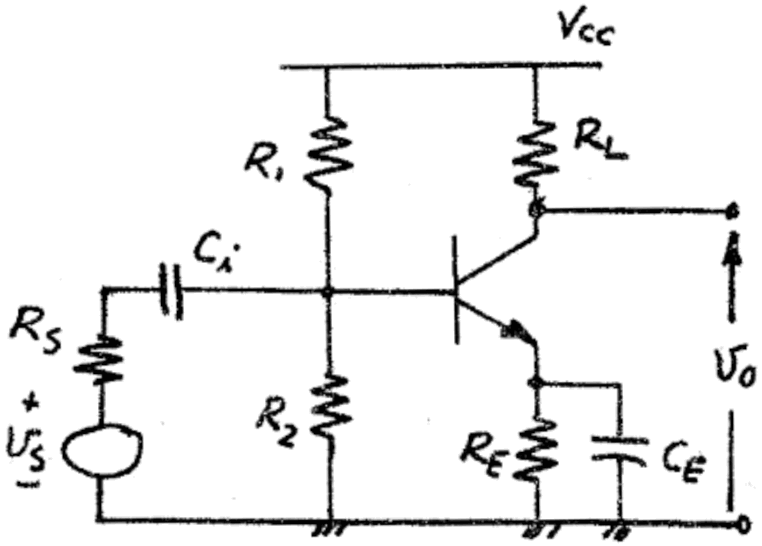
\includegraphics[width=0.26\linewidth]{_fig/respfreq_ejemplo_t-hf-ec_conf.png}
		\label{fig:respfreq_ejemplo_t-hf-ec_conf}
	}
	\subfloat[Circuito para frecuencias medias y altas]
	{
		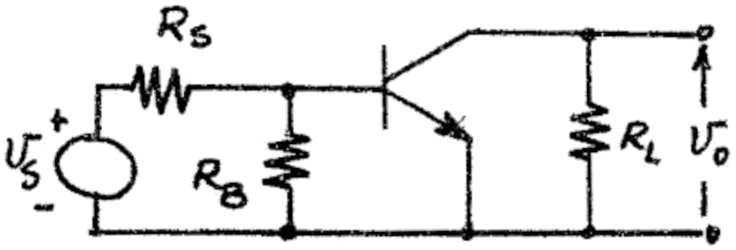
\includegraphics[width=0.33\linewidth]{_fig/respfreq_ejemplo_t-hf-ec_mf-hf.png}
		\label{fig:respfreq_ejemplo_t-hf-ec_mf-hf}
	}
	\subfloat[Circuito con Modelo]
	{
		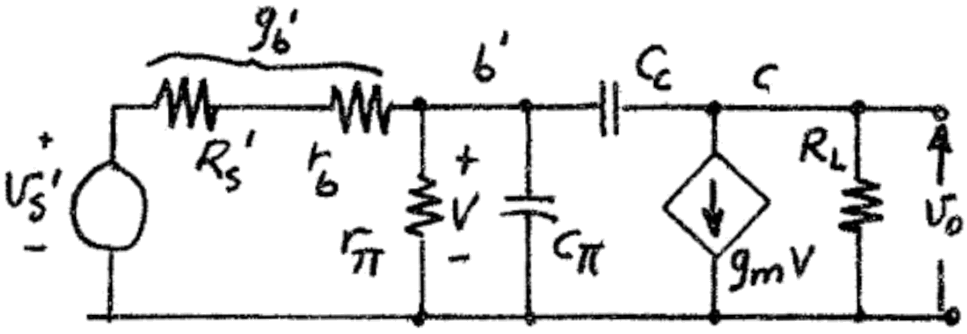
\includegraphics[width=0.37\linewidth]{_fig/respfreq_ejemplo_t-hf-ec_con-modelo.png}
		\label{fig:respfreq_ejemplo_t-hf-ec_con-modelo}
	}
	\caption{Análisis de Alta Frecuencia para E.C.}
	\label{fig:respfreq_ejemplo_t-hf-ec}
\end{figure}

de donde:

\[ V_o = \frac{-g_b' V_S' (g_m - s C_c)}{(g_\pi + s C_\pi + g_b' + {s C_c}) (s C_c + G_L) - (-s C_c) (g_m - s C_c)} \]

ó,

\begin{equation} \label{respfreq_transistor_funcion-transferencia}
	\frac{V_o}{V_S'} (s) = \frac{-g_b' (g_m - s C_c)}{s^2 C_\pi C_c + s (C_\pi G_L + C_c (g_m + G_L g_\pi + G_L g_b)) + (g_\pi + g_b') G_L}
\end{equation}

Esta es la función de transferencia completa para medias y altas frecuencias de donde se puede hallar los polos y los ceros de \( V_o / V_S' (s) \).

Se ha demostrado que el modelo híbrido es solo válido para

\begin{equation} \label{respfreq_transistor-pi-hibrido_valido}
	\omega < \omega_T / 3
\end{equation}

Mas alla de esta frecuencia, se requiere de modelos mas sofisticados del transistor. Dado la ecuación \ref{respfreq_transistor-pi-hibrido}, la ecuación \ref{respfreq_transistor-pi-hibrido_valido} es equivalente a:

\begin{equation}
	\omega < \frac{g_m}{(C_\pi + C_c) 3}
\end{equation}

Expresado de otra forma, el modelo híbrido es válido solo para:

\begin{equation}
	\omega C_c + \omega C_\pi << g_m
\end{equation}

que a su vez implica:

\begin{equation}
	\omega C_\pi << g_m
\end{equation}

\begin{equation}
	\omega C_c << g_m
\end{equation}

De la ecuación \ref{respfreq_transistor_funcion-transferencia} se puede despreciar el termino \( s^2 C_\pi C_c \) ya que \( s^2 C_\pi C_c << g_m s C_c \) y se desprecia en el numerador \( s C_c \). Entonces queda:

\begin{equation}
	\frac{V_o (s)}{V_S} \approx \frac{-g_m g_m}{s [C_\pi G_L + C_c (g_m + G_L + g_b')] + (g_\pi + g_b') G_L}
\end{equation}

Para expresarlo de la forma deseada, \( V_o (s) = K \frac{1}{1 + s \tau} \), sacamos el factor \( G_L (g_\pi + g_b') \) y queda:

\begin{equation} \label{respfreq_transistor_funcion-transferencia_vo-ss}
	\frac{V_o (s)}{V_S} = \frac{-g_m g_m R_L}{g_\pi + g_b'} \frac{1}{1 + s \frac{C_\pi + C_c (1 + R_L (g_m + g_b'))}{g_\pi + g_b'}}
\end{equation}

Por lo tanto, el polo de alta frecuencia viene dado por:

\begin{equation} \label{respfreq_transistor_gain-hf}
	\omega_A = \frac{1}{R_T C_A} = \frac{g_\pi + g_b'}{C_\pi + C_c (1 + R_L (g_m + g_\pi + g_b'))}
\end{equation}

La ganancia a frecuencias medias viene dada por:

\begin{equation} \label{respfreq_transistor_gain-mf}
	A = \frac{-g_m R_L}{g_\pi + g_b'} = -\frac{g_m R_L}{1/r_\pi + 1/R_S'} = \frac{-\beta R_L}{r_\pi + R_S'}
\end{equation}

Esta expresión es la misma que se consigue para la ganancia de la configuración E.C. utilizando el modelo simplificado.

\begin{figure}[h]
	\centering
	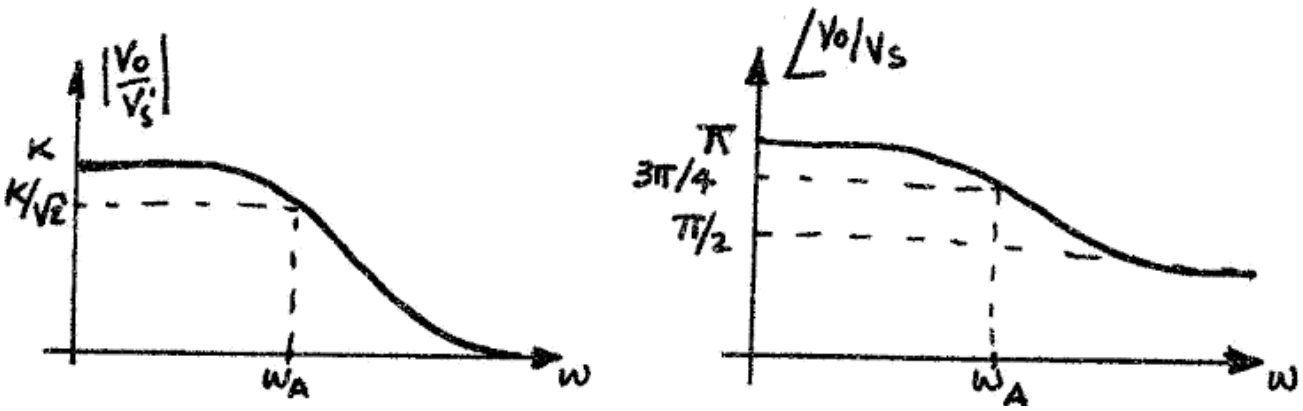
\includegraphics[width=0.8\linewidth]{_fig/respfreq_ejemplo_resp_funcion-transferencia.png}
	\caption{Respuesta de la Funcion de la Ecuación \ref{respfreq_transistor_gain-mf}}
	\label{fig:respfreq_ejemplo_resp_funcion-transferencia}
\end{figure}

En la Figura \ref{fig:respfreq_ejemplo_resp_funcion-transferencia} se muestra la respuesta de la Ecuación \ref{respfreq_transistor_funcion-transferencia_vo-ss}. Si ahora se toma en cuenta la contribución a la función de transferencia debido a \( C_i \) y \( C_E \) se consigue:

\begin{equation} \label{respfreq_transistor_resp-equ}
	\frac{V_o}{V_S} (s) = K \frac{s}{s + \omega_1} \frac{s \omega_2}{s + \omega_3} \frac{1}{1 + s \tau_A}
\end{equation}

\begin{figure}[h]
	\centering
	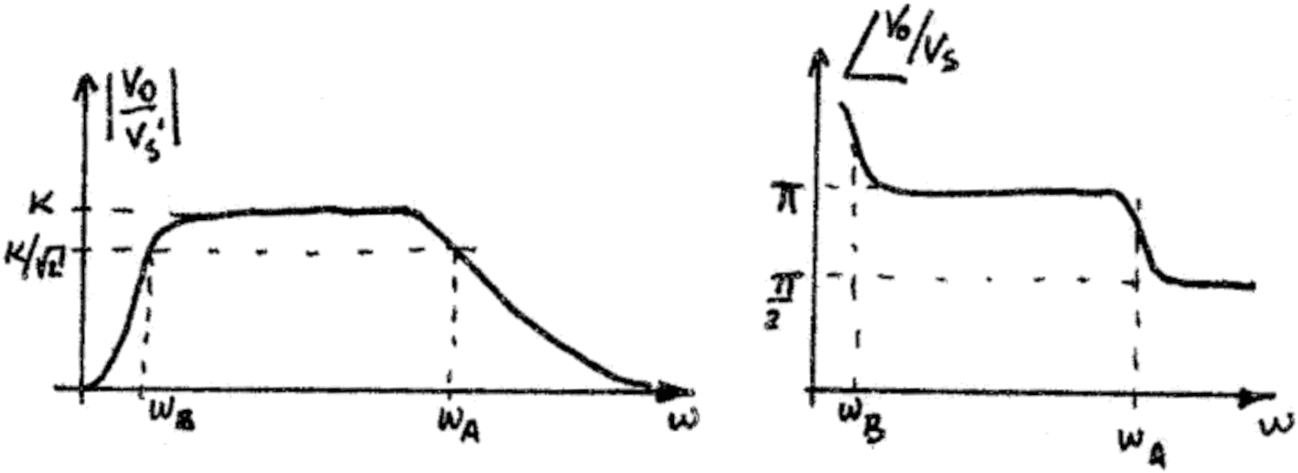
\includegraphics[width=0.8\linewidth]{_fig/respfreq_ejemplo_resp_funcion-transferencia-eq.png}
	\caption{Respuesta de la Función de la Ecuación \ref{respfreq_transistor_resp-equ}}
	\label{fig:respfreq_ejemplo_resp_funcion-transferencia-eq}
\end{figure}

que se grafica en la Figura \ref{fig:respfreq_ejemplo_resp_funcion-transferencia-eq}.

Además la expresión para la frecuencia de corte alta, la Ecuación \ref{respfreq_transistor_gain-hf}, tiene una interpretación circuital muy interesante.

donde \( g_\pi + g_b' = \frac{1}{r_\pi \parallel R_S'} \). Y se desprecia \( g_\pi + g_b' \) que generalmente cumplen la condición \( g_\pi + g_b' << g_m \). El circuito que tiene este polo, y la ganancia dada en la Ecuación \ref{respfreq_transistor_gain-mf} se muestra en la Figura \ref{fig:respfreq_resp-simple-conf-ec}. El polo viene dado por \(-1 / R_T C_T\) donde \( R_T \) es la resistencia de Thevenin vista desde los extremos de la capacitancia total:

\[ C_\pi + C_c (1 + g_m R_L) \]

\begin{figure}[h]
	\centering
	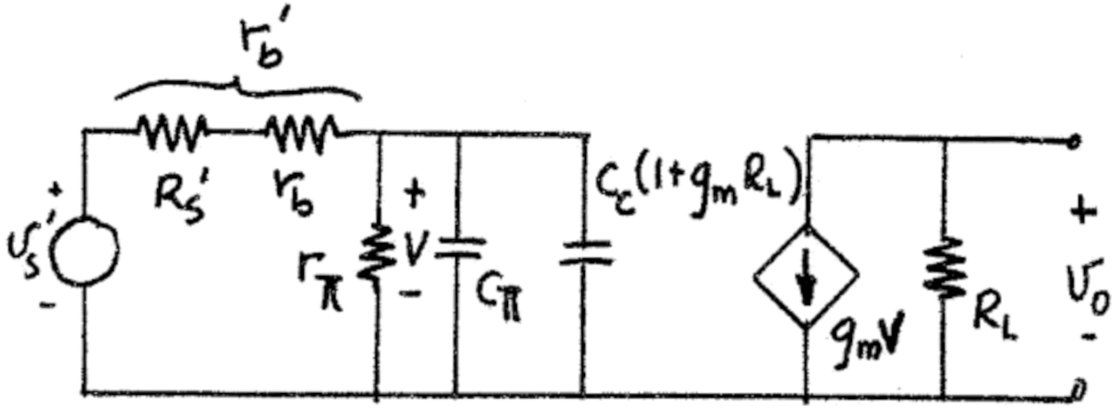
\includegraphics[width=0.8\linewidth]{_fig/respfreq_resp-simple-conf-ec.png}
	\caption{Interpretación circuital sencilla para configuración E.C.}
	\label{fig:respfreq_resp-simple-conf-ec}
\end{figure}

La capacitancia \( C_c (1 + g_m R_L) \) forma parte de la capacitancia de entrada y domina la capacitancia de Miller ya que corresponde a la calculada partiendo del Teorema de Miller, planteado en la Figura \ref{fig:respfreq_teorema-miller}. El teorema establece que las tensiones y corrientes en una red permanecen iguales si cualquier impedancia Z entre dos nodos con voltajes \( V_1 \) y \( V_2 \), se transforma en dos impedancias a tierra de valores \( Z' = Z / (1 - V_2 / V_1) \) del nodo \( V_1 \), y \( Z'' = Z / (1 - V_1 / V_2) \) del nodo \( V_2 \).

\begin{figure}[h]
	\centering
	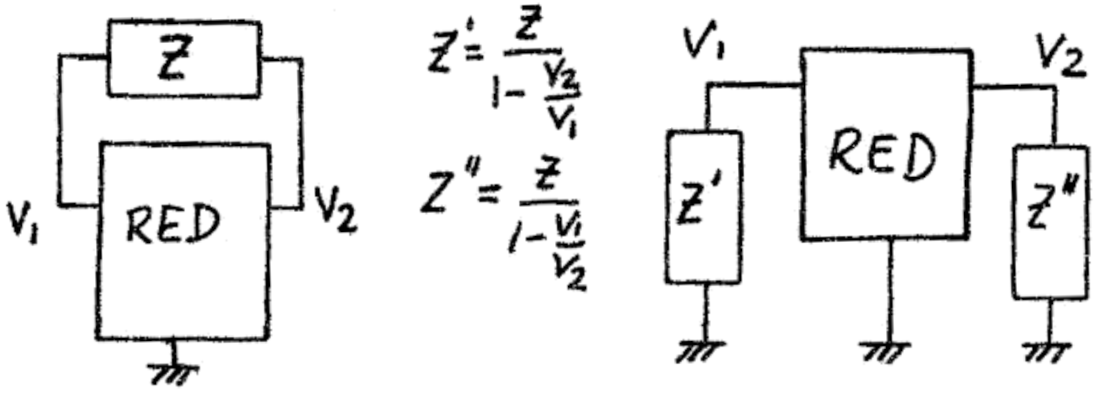
\includegraphics[width=0.8\linewidth]{_fig/respfreq_teorema-miller.png}
	\caption{Teorema de Miller}
	\label{fig:respfreq_teorema-miller}
\end{figure}

Del circuito de la Figura \ref{fig:respfreq_ejemplo_t-hf-ec_con-modelo}, se determina que la ganancia \( V_o / V = -g_m R_L \). Entonces se puede llevar \( C_c \) a su equivalente en paralelo con \( C_\pi \) con valor \( C_c (1 + g_m R_L) \) ya que:

\[ Z' = \frac{Z}{1 - \frac{V_o}{V}} = \frac{1}{s C_c (1 - (-g_m R_L))} = \frac{1}{s C (1 + g_m R_L)} \]

A pesar de que \( C_c \) es una capacitancia pequeña su efecto sobre el polo de alta frecuencia es tan apreciable como \( C_\pi \) debido al factor multiplicador \( (1 + g_m R_L) \).

Se hace notar que aplicando el Teorema de Miller se crea otra capacitancia en paralelo con \( R_L \), pero su efecto es despreciable como veremos en el próximo ejemplo.

\subsubsection{Ejemplo 6} \label{respfreq_ejm6}
Hallar la ganancia y la frecuencia de corte alta para el circuito de la Figura \ref{fig:respfreq_ejemplo_t-ec_autopolarizado}.

\textbf{Solución.} En la figura 1.61 se plantea el circuito apto para este análisis, en donde se parte del circuito de la figura 1.55 con los condensadores \( C_i \) y \( C_E \) cortocircuitados, y con \( R_S = 50 \).

\begin{figure}[h]
	\centering
	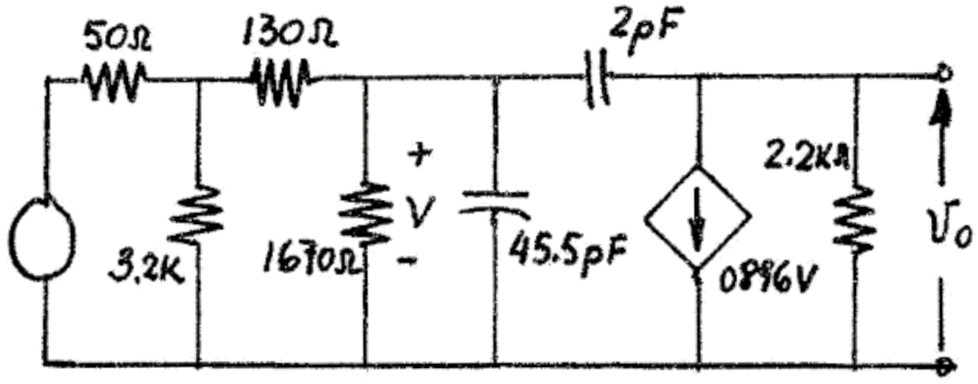
\includegraphics[width=0.8\linewidth]{_fig/respfreq_ejemplo_t-ec_autopolarizado_mf-hf.png}
	\caption{Circuito de la Figura \ref{fig:respfreq_ejemplo_t-ec_autopolarizado} para medias y altas frecuencias}
	\label{fig:respfreq_ejemplo_t-ec_autopolarizado_mf-hf}
\end{figure}

Entonces:

\[ A_M = \frac{-\beta R_L}{r_\pi + R_S} = \frac{-150 \times 2.2 \text{ k}}{1800 + 99.2} = -178 \]

el polo dominante:

\[ \omega_A = \frac{g_\pi + g_b'}{C_\pi + C_c (1 + g_m + g_\pi + g_b') R_L} \]

\[ \omega_A = \frac{0.00618}{45.1 \times 10^{-12} + 2.2 \times 10^{-12} (1 + (0.00618 + 0.0896) 2.2 \times 10^3)} = 13.2 \text{ MR/s } (f_A = 2.1 \text{ MHz}) \]

y el segundo polo:

\[ \omega_{A2} = \frac{1}{R_L C_c} = \frac{1}{2.2 \times 10^3 \times 2 \times 10^{-12}} = 227 \text{ MR/s } (\text{casi } 20 \omega_A) \]

\subsubsection{Ejemplo 7} \label{respfreq_ejm7}
Si \( R_L \) cambia a \( 1.1K \), con \( I_C \) igual y \( V_{CE} = 5.6 \) se tiene \( C_c = 1.9 pF \). Entonces, \( A_M = -89 \) y \( \omega_A = 25 MR/s \).

Una comparación de las ganancias y frecuencias de corte alta obtenidas en los Ejemplos \ref{respfreq_ejm6} y \ref{respfreq_ejm7} demuestra la relación inversa entre ganancia y ancho de banda que siempre se presenta en los amplificadores electrónicos: si uno aumenta, la otra disminuye.

\subsubsection{Ejemplo 8} \label{respfreq_ejm8}
Hallar la función de transferencia general y los valores específicos de la ganancia y la frecuencia de corte alta de la configuración colector común de la Figura \ref{fig:respfreq_conf-colector-comun}.

\begin{figure}[h]
	\centering
	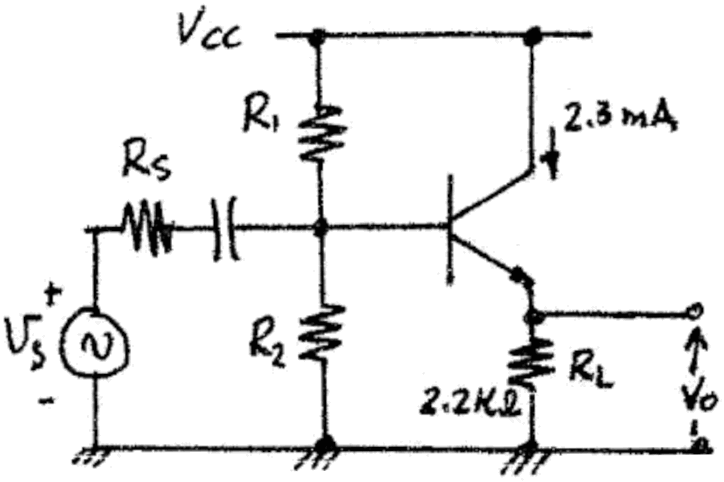
\includegraphics[width=0.5\linewidth]{_fig/respfreq_conf-colector-comun.png}
	\caption{Configuración Colector Común}
	\label{fig:respfreq_conf-colector-comun}
\end{figure}

El mismo procedimiento que se aplicó a la configuración E.C. se podría aplicar ahora a las demás configuraciones.

Para altas, el circuito de la Figura \ref{fig:respfreq_conf-colector-comun} queda como en la Figura \ref{fig:respfreq_conf-colector-comun_hf}.

\begin{figure}[h]
	\centering
	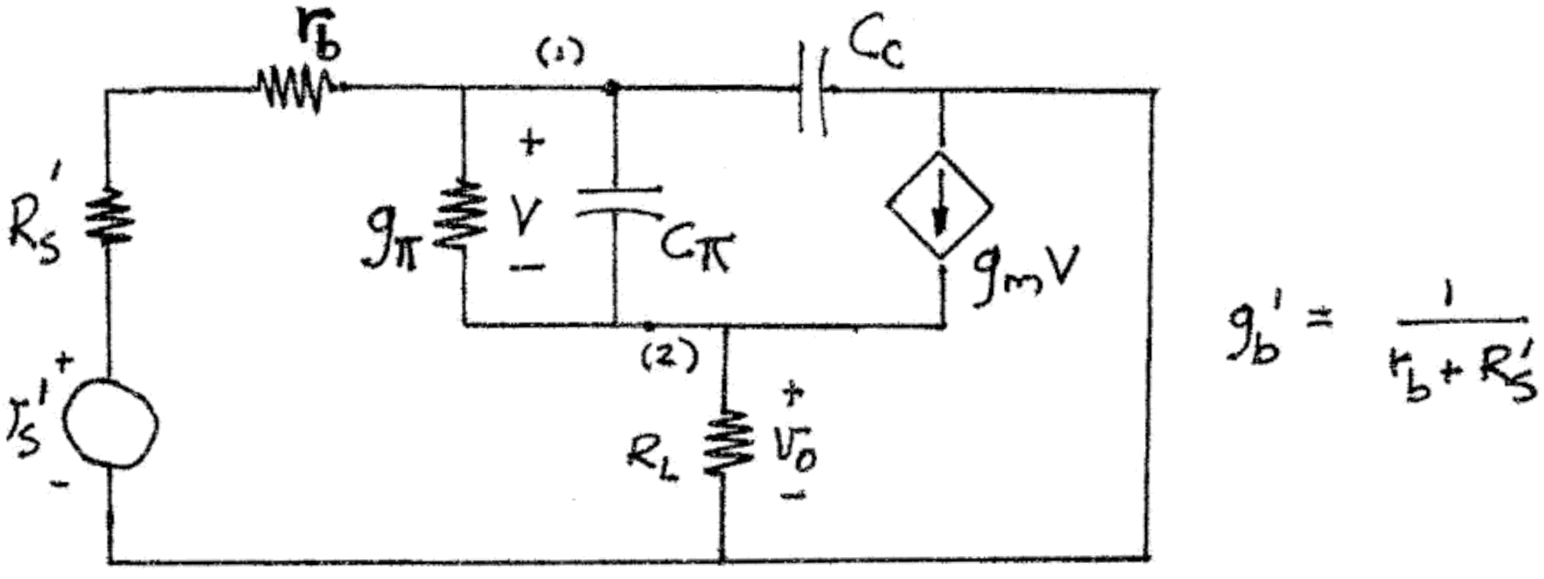
\includegraphics[width=0.8\linewidth]{_fig/respfreq_conf-colector-comun_hf.png}
	\caption{Amplificador Configuración Colector Común para Altas Frecuencias}
	\label{fig:respfreq_conf-colector-comun_hf}
\end{figure}

Entonces:

1) \( (V + V_o - V_S) g_b' + V (g_\pi + s C_\pi) + (V + V_o) s C_c = 0 \)

2) \( -V(g_\pi + s C_\pi + g_m) + V_o g_L = 0 \)

Luego:

1) \( V(g_b' + g_\pi + sC_c) + V_o(g_b' + sC_c) = V_s' g_b' \)

2) \( V = \frac{V_o g_L}{g_\pi + sC_\pi + g_m}  \approx \frac{V_o g_L}{g_m} \)

Finalmente:

\[ V_o \left[ \frac{g_L (g_b' + g_\pi + sC_c + sC_\pi)}{g_m} + g_b' + s C_c \right] = V_s' g_b' \]

ó

\[ \frac{V_o}{V_s'} = \frac{g_m g_b'}{g_L (g_b' + g_\pi) + g_m g_b' + g_L (s C_c + s C_\pi) + g_m s C_c} \]

de donde

\[ \frac{V_o}{V_s'} = \frac{g_m g_b'}{g_L (g_b' + g_\pi) + g_m g_b'} \frac{1}{1 + s \left[ \frac{g_L (C_c + C_\pi) + g_m C_c}{g_L (g_b' + g_\pi) + g_m g_b'} \right]} \]

\[ \frac{V_o}{V_s'} = A_M \frac{1}{1 + s \tau_A} \]

Dado valores del Ejemplo \ref{respfreq_ejm2} (caso E.C.) y \( R_L = 2.2K \), se obtiene \( g_L = 0.000455 \), \( g_m = 0.0896 \), \( g_b' = 0.00558 \), \( g_\pi = 0.0006 \), \( C_c = 2.4 pF \), \( C_\pi = 45.1 pF \). Entonces:

\[ A_M = \frac{0.0896 + 0.00558}{0.000455 (0.00558 + 0.0006) + (0.0896) (0.00558)} = 0.999 \]

\[ \omega_A = \frac{0.000455 (0.00558 + 0.0006) + (0.0896) (0.00558)}{(0.000455) (47.5 \times 10^{-12}) + (0.0896) (2.4 \times 10^{-12})} = 2.1 \times 10^9 \]

\section{Problemario} %p59
- pendiente en apuntes -